\documentclass[11pt]{article} 

\usepackage[letterpaper,left=1in,right=1in,top=1.4in,bottom=1.5in]{geometry}

% packages i use in essentially every document
\usepackage{graphicx}
\usepackage{enumerate}
\usepackage{booktabs}
\usepackage{lipsum}
\usepackage{lscape}
\usepackage{dcolumn}
\usepackage{amsmath}
\usepackage{comment}

\usepackage[utf8]{inputenc}

%%\usepackage[center]{caption}
\DeclareUnicodeCharacter{00A0}{ }

\usepackage{fancyhdr}
\usepackage{changepage}
\pagestyle{fancy}
\renewcommand{\headrulewidth}{0pt}
\fancyhf{}
\fancyhead[R]{\thepage}

%% prevent images from floating
\usepackage{placeins}

% packages i use in many documents but leave off by default
\usepackage{amsmath, amsthm, amssymb}
%\usepackage{amsmath}
% \usepackage{dcolumn}
% \usepackage{endfloat}


% import and customize urls (kjh does this as well, it seems)
\usepackage[usenames,dvipsnames]{color}
\usepackage[breaklinks]{hyperref}

\hypersetup{colorlinks=true, linkcolor=Blue, citecolor=Black, filecolor=Blue,
    urlcolor=Blue, unicode=true}

\usepackage[center, textfont={bf}, labelsep=period, format=hang]{caption}

%\DeclareCaptionFormat{upper}{#1#2\uppercase{#3}\par}
%\captionsetup{labelsep=period, format = upper, singlelinecheck = false, skip = 2pt,figurename=FIGURE}

\setlength{\parindent}{0pt}
\baselineskip 18.5pt
%\setlength{\parskip}{4.5pt}
\setlength{\parskip}{8pt}

%\linespread{1.45}
\linespread{1.2}

\pdfminorversion 3


% add bibliographic stuff 
\usepackage[round]{natbib}
\def\citepos#1{\citeauthor{#1}'s (\citeyear{#1})}
\def\citespos#1{\citeauthor{#1}' (\citeyear{#1})}

% import vc stuff after running `make vc`: \input{vc} \pagestyle{kjhgit}

\begin{document}

\setlength{\parskip}{4.5pt}

\baselineskip 18.5pt

\title{Does Copyright Affect Reuse?\\ Evidence from the Google Books Digitization Project}
%\title{Does Copyright Limit Gains From Digitization?\\ Evidence from Google Books and Wikipedia}

%%\footnote{I am thankful to Erik Brynjolfsson, Daniel Fehder, Jeff Furman, Shane Greenstein, Joshua Krieger, Matt Marx, Aruna Ranganathan, Fabian Waldinger, Pai-Ling Yin, participants of the Economic Sociology Working Group and MIT Economics Third Year Lunch and especially Pierre Azoulay, Scott Stern, Catherine Tucker and Heidi Williams for comments. All errors remain mine.}


\author{Abhishek Nagaraj \footnote{MIT Sloan School of Management. E62-368, 100 Main Street, Cambridge, MA 02139. I am thankful to Erik Brynjolfsson, Daniel Fehder, Jeff Furman, Avi Goldfarb, Shane Greenstein, Joshua Krieger, Matt Marx, Aruna Ranganathan, Fabian Waldinger, Pai-Ling Yin, participants of the Economic Sociology Working Group and MIT Economics Third Year Lunch and especially Pierre Azoulay, Scott Stern, Catherine Tucker and Heidi Williams for comments. All errors remain mine.}
\\         \texttt{nagaraj@mit.edu}   
}

%%\date{\today}
\date{May 8, 2016}

\maketitle
\thispagestyle{empty}


\begin{abstract}
\normalsize
While digitization projects like Google Books have dramatically increased access to information, this study examines how the ability to reuse digital information and diffuse knowledge to a wider audience critically depends on features of copyright law. I use the digitization of both copyrighted and non-copyrighted issues of \emph{Baseball Digest} by the Google Books Digitization Project to measure the impact of copyright on a prominent venue for reuse: Wikipedia. A specific feature of the 1909 Copyright Act, \emph{copyright renewal requirements} ensure that material published before 1964 is out of copyright, which allows for causal estimation of the impact of copyright on Wikipedia across this sharp cutoff. I find that digitization by Google Books increased the reuse of Baseball Digest on Wikipedia, but copyright hurt reuse by reducing citations to copyrighted issues by over 135\%. Copyright also had real impacts on readership -- affected pages had, on average, 20\% lower gains in internet traffic than pages unaffected by copyright. Finally, the impact of copyright on digitized material was highly uneven. Copyright mostly affected the reuse of images rather than text, and prevented reuse of information about less-popular players as compared to more popular ones. 


%%I hypothesize and find that 
%%Copyright mostly prevented the reuse of images rather than text, and copyright significantly hurt the quality of Wikipedia pages for less-popular baseball players compared to their more popular counterparts. 

%%However, the negative impact of copyright on diffusion is more pronounced for images compared to text and becomes large only when costs of access to digital material are reduced through the Google Books project. %%The main contribution of this paper is to provide the first causal estimates of the impact of copyright on reuse, a key measurement for copyright policy. 
\end{abstract}

%% I exploit a specific feature of the 1909 Copyright Act, \emph{copyright renewal} requirement, which caused issues of one magazine \emph{Baseball Digest} published before 1964 to fall in the public domain, while issues published after 1964 retained their copyright for this exercise. Specifically, 

\setcounter{page}{1}
\pagenumbering{arabic}

\newpage
\section{Introduction}

The increasing digital representation of information has impacted a wide range of economic activities \citep{greenstein_digitization_2013}. Digitization has reduced the cost of storage, computation and transmission of information and enabled massive changes in the ways that creative producers build upon and reuse existing information  \citep{goldfarb_introduction_2014}. For example, the digitization of music has enabled new forms of production, remixing and reuse which has resulted in a new wave of innovation in the music industry \citep{waldfogel_digitization_2014}. Similarly, the digitization of ``prior art'' about traditional medicine has significantly affected new innovations in this area \citep{choudhury_ex-ante_2015}. 

%Similarly, the availability of new digital maps of the earth's surface have led to a new wave of discoveries in the gold exploration industry \citep{nagaraj_private_2015}.

%There remains significant potential for the wider diffusion of digital information to transform markets in the near future. 

Despite its enormous potential, the digitization process is governed by intellectual property and copyright laws that were originally conceptualized for more traditional forms of content. Therefore, the question of whether and how copyright should be modified for the digital age has become a prominent topic of discussion in policy and legal circles \citep{merges_intellectual_2012}. Some firms have argued for strengthening of copyright protection given the difficulties in enforcing copyright on digital information \citep{anderson_new_2007}, while others have argued that the current copyright regime severely undermines reuse and, therefore, limits the economic potential of digitization \citep{samuelson_intellectual_1999, lessig_free_2004}. Despite the economic importance of these debates (for example, see Supreme Court case \emph{Authors Guild v. Google, Inc.}), there is little empirical evidence about whether and how copyright influences the diffusion and reuse of digital information. A recent essay describing gaps in the literature summarizes this problem quite succinctly ``[we understand little about] what would be the economic effects of various alternative copyright arrangements and proposals for its redesign'' \citep{greenstein_digitization_2013}.

Theoretically, it is difficult to predict how copyright would affect the possible gains from the digitization process. According to IP prospect theory \citep{kitch_nature_1977}, broad and strong intellectual property is needed to spur reuse by facilitating the licensing and maintenance of information \citep{mazzoleni_economic_1998, gallini_intellectual_2002} in the face of digital piracy \citep{rob_piracy_2007}, while transaction cost theories predict that when digitization reduces costs of access, copyright could significantly hinder reuse \citep{lessig_free_2005, benkler_wealth_2006, zittrain_future_2009, lemley_ex_2004}. While diametrically opposed, the two theories are clear in their respective predictions: according  to  one  theory, copyright lubricates  the  market for ideas \citep{gans_product_2003} and needs to be strengthened in the face of digitization, while according to the other, digitization impedes the free diffusion of digital information and needs to be reigned-in. Further, given contradictory theoretical predictions, empirical research on the impact of copyright on reuse also faces significant challenges. First, it is difficult to cleanly measure the reuse and diffusion of digital information. Second, there exists little variation in copyright -- it often applies by default for over a hundred years. And finally, even when variation exists, comparing the reuse of out-of-copyright and in-copyright material is problematic because such variation is often correlated with the quality or recency of the underlying material. 

%%While diametrically opposed, these two theories are clear in their respective predictions; according to one theory, copyright lubricates the digital market for ideas, and, according to the other, it impedes the free diffusion of digital information.

%%Prospect theory \citep{kitch_nature_1977, hardin_tragedy_1968, landes_indefinitely_2002,liebowitz_seventeen_2004} holds that broad and strong intellectual property rights are useful, because they both incentivize the creation of new knowledge \citep{gans_remix_2014} and spur reuse by reducing contracting costs for the licensing of existing digital information by stimulating the maintenance of works already created (\cite{mazzoleni_economic_1998}, \cite{gallini_intellectual_2002}, \cite{gans_is_2010}, \cite{arora_markets_2001}). However, under a competing logic, copyright imposes transaction costs that prevent the exchange of information. These transaction costs are likely to be 

%% Given contradictory theoretical predictions, systematic empirical analysis of the impact of copyright on reuse could help make progress on this question. Unfortunately, such analysis has largely been absent in the innovation and management literature on the topic, perhaps due to empirical challenges. Issues of data and measurement are central. Unlike scientific output which can be measured through patents and the publication record, the diffusion of cultural information is more informal and harder to track. When data can be located, copyright applies to all information by default and persists often for over a hundred years. This, makes it rather difficult to observe diffusion in the absence of copyright. Finally, even if these problems can be resolved, comparing reuse of copyrighted and non-copyrighted information is challenging because unobserved variables like the underlying quality of information are often correlated with reuse. Put another way, we do not know if information was reused because it was off-copyright or because it was inherently of higher quality. 


%%Previous work in copyright has been largely theoretical and has focused on estimating the elasticity of new creative products with the strength of copyright protection (\cite{varian_copyright_2006}, \cite{watt_copyright_2006}). However, because digital  the creative process is cumulative in many markets (\cite{williams_intellectual_2013}, \cite{furman_climbing_2011}, \cite{scotchmer_standing_1991}), copyright may also affect reuse by changing the cost of reusing creative inputs in the production of new knowledge (\cite{li_dead_2012}, \cite{lerner_lost_2012}). This second impact is the focus of this study. 

%% According to existing theory, whether copyright impedes or promotes the reuse of knowledge is unclear. 

In this paper, I make empirical progress on the question of the impact of copyright on the reuse of digital information by exploiting a natural experiment that occurred during a marquee project in the history of the internet: the digitization of about 30 million works by Google Books. About 4 years after the project was underway, in December 2008, Google Books digitized all existing issues (i.e. every issue published between 1940 to 2008) of \emph{Baseball Digest}, a prominent baseball magazine, and made them available online to readers for free. The digitization of \emph{Baseball Digest} is particularly relevant for this study, because, due to an accidental failure to renew copyrights, issues of the magazine published before 1964 lapsed into the public domain. Consequently, pre-1964 \emph{Baseball Digest} issues can be freely reused, while those published after 1964 are copyrighted and their reuse, without permission is legally prohibited. At the same time, however, both pre-1964 and post-1964 issues of the magazine were digitized by Google Books and could be accessed and read online. By exploiting this idiosyncratic variation in copyright, this study sheds light on the broader question of how intellectual property could affect the potential benefits from digitization. In particular, I focus on the impact of copyright on affecting the reuse of magazine material on Wikipedia, a natural venue to investigate this question. Not only is Wikipedia the fifth most visited website on the internet (receiving about 10 billion page-views every month) as well as a common source of information about the history of baseball, it also stores all past versions of a given page, allowing the analyst to track how information changes in response to the Google Books digitization event and copyright. 

To make things clearer, consider the example in Figure~\ref{fig:cover}. The example shows scanned pages from Google Books for two issues of \emph{Baseball Digest}. Panel (1) is about a feature on Felipe Alou published in 1963, rendering it ``out-of-copyright'', while Panel (2) is on Johnny Callison published in 1964, making it ``in-copyright.'' For these two players, Figure~\ref{fig:cover} depicts pages on Wikipedia as they appeared in December 2012. Neither of these two pages displayed the players' images before \emph{Baseball Digest} was digitized, but in 2012, while Alou's page had an image from Baseball Digest, Callison's page had no images at all. Despite being printed in two issues that were published around the same time, one image finds use in a broader context while the other seems lost among the pages of Baseball Digest. Further analysis shows that, over 51 new citations were made between 2008 and 2012 to issues of Baseball Digest published in 1963, while only 17 new citations were made to magazine issues published in 1964 in the same time period. Furthermore, at the page level, Felipe Alou's Wikipedia page in 2012 contained a citation to the 1963 issue of \emph{Baseball Digest}, and experienced about a 121\% increase in traffic since 2008 as compared to only a 23\% increase for Callison's page. While many alternative explanations (such as differences in player popularity) could account for the differences, the statistical analysis isolates the role of copyright in establishing these patterns.

Specifically, I track Wikipedia citations to issues of Baseball Digest published between 1944 and 1984 before and after the Google Books project on Wikipedia (i.e. between 2004 and 2012). The unit of analysis is a ``publication-year,'' i.e. all issues of the magazine published in any given year between 1944 and 1984. Using these data, I estimate whether out-of-copyright magazine issues (publication-years 1944-1963), were disproportionately more likely to be cited on Wikipedia as compared to in-copyright issues (publication-years 1964-1984) after the Google Books digitization event in a differences-in-differences framework. This specification helps to isolate the causal impact of copyright on the reuse of Baseball Digest information after the launch of the digitization project. 

Figure \ref{fig:overview} provides some simple descriptive statistics that foreshadow the core econometric results. Panel (1) plots total citations to all issues of Baseball Digest on Wikipedia between 2004-2012, while Panel (2) plots total citations separately for in-copyright and out-of-copyright publication-years. As Panel (1) indicates, after the digitization of Baseball Digest in late 2008, the average number of citations for all publication-years of the magazine between 1944-1984 increased dramatically, suggesting the large and positive impact of digitization on information reuse. However, when this increase is examined separately in Panel (2) for in-copyright and out-of-copyright publication-years, the gains from digitization are heavily concentrated for out-of-copyright issues. The econometric estimates indicate that citations to out-of-copyright publication-years increase by about 135\% as compared to citations to in-copyright publication-years after digitization, even after controlling for publication-year and calendar-year fixed effects. Combined, Figure \ref{fig:overview} and the econometric estimates convey the headline findings of the paper -- the digitization project greatly encouraged the reuse of Baseball Digest information on Wikipedia, but information from copyrighted issues was significantly less likely to be reused. 

Having understood the impact of the copyright law at the publication-year level, I construct an additional sample at the Wikipedia player-page level (Sample B) which tracks Wikipedia pages for a set of about five hundred prominent baseball players who were active between 1944 and 1984. Using this sample I provide robustness for the baseline analysis and extend it in two different ways. First, I evaluate the impact of copyright on the value that Wikipedia pages deliver to end users, by incorporating data on user traffic to Wikipedia pages. If, despite the limited diffusion of information from in-copyright Baseball Digest issues, Wikipedia editors are able to create high-quality pages using information from alternate sources and attract similar levels of readership, then the welfare consequences of copyright on Wikipedia are likely to be less severe. However, my econometric estimates indicate that pages affected by copyright had on average 20\% lower gains in internet traffic, suggesting a permanent and significant loss to Wikipedia from the inability to reuse copyrighted information. 

Second, I hypothesize and test the idea that while copyright lowers the overall level of reuse, its impact is more concentrated for certain types of information as compared to others. Building on the digitization and intellectual property literature, I argue that the impact of copyright on preventing reuse is most salient when the underlying information is harder to duplicate using alternate sources. Specifically, I hypothesize that the impact of copyright is most salient for the reuse of images rather than text because it is harder to duplicate visual information without violating copyright, while textual information is easily paraphrased. Similarly, I also hypothesize that copyright restrictions on digital information are most harmful for Wikipedia pages about players who are less well-known because information about them is harder to obtain from alternate sources. I test the heterogeneous impact of the 1964-copyright experiment on both these margins in a regression framework and find support for my hypotheses. These results highlight the important role of copyright law in affecting digitization by shaping the distribution of reuse for different types of information. 

This research contributes to the literature on digitization \citep{goldfarb_effect_2012, miller_can_2011, waldfogel_digitization_2014} by evaluating the role of intellectual property law in influencing the economic impacts of digitization. I show, for the first time, how copyright law could severely curtail potential benefits of digitization in online contexts. I also add to research on the role of digitization in influencing the differences in outcomes between more and less established players in a market \citep{qian_counterfeiters:_2014, mortimer_supply_2012, zhang_intellectual_2014, nagaraj_private_2015, brynjolfsson_niches_2006}. Finally, I also contribute to the nascent empirical literature on copyright including some work in the legal domain estimating the impact of copyright in the publishing context \citep{heald_property_2007, heald_testing_2009, buccafusco_bad_2012}, work that studies the impact of copyright on prices \citep{li_dead_2012, reimers_effects_2013, mortimer_price_2007-2} and literature on copyright enforcement and piracy \citep{aguiar_digitization_2014, luo_copyright_2015-1, danaher_converting_2010}.

The rest of the paper is organized as follows. Section \ref{sec:setting} describes the empirical setting including the \emph{Baseball Digest} experiment and data collection. Section \ref{sec:baseline} analyzes the overall impact of the \emph{Baseball Digest} copyright experiment, while Section \ref{sec:hetero} discusses distributional impacts. Finally, Section \ref{sec:discussion} concludes. 


%%is also relevant. This paper adds to this literature by focusing on the causal impact of copyright on \emph{reuse}, by using micro-data on knowledge flows and by separately identifying the interaction between digitization and copyright. 

%% The findings that there are heterogeneous impacts on players of different qualities are interesting and relate to a few past studies: a. Napster helped concert revenue of less popular singers more than the established singers (Mortimer et. al. 2014), b. counterfeiting has a larger advertisement effect for the brands that were less well-known at the time of infringement and newer brands that had less sub-brands (Qian 2014).

%%In sum, I find that while digitization projects can help the broader diffusion of knowledge, copyright can have negative impacts on reuse. More broadly, this research shows how copyright policy can strongly influence the rate and direction of follow-on innovation on the internet. The present study joins the literature on digitization by pointing out the important role of intellectual property in influencing the impact of digital information on economic outcomes. Further, I also contribute more broadly, to the nascent empirical literature on copyright as well as related work on innovation, digitization and privacy. Of note is work in the legal literature on copyright that estimates the impact of copyright on availability and compares works produced before and after the US copyright cutoff date of 1923 \citep{heald_property_2007, heald_testing_2009, buccafusco_bad_2012}. Other work that studies the impact of copyright on prices and access in the market for historical books \citep{li_dead_2012, reimers_effects_2013} is also relevant. This paper adds to this literature by focusing on the causal impact of copyright on \emph{reuse}, by using micro-data on knowledge flows and by separately identifying the interaction between digitization and copyright. Finally, this paper contributes to a broader literature on knowledge flows (\cite{agrawal_gone_2006}, \cite{catalini_microgeography_2012}, \cite{singh_geographic_2013}) and the role of intellectual property (\cite{murray_formal_2007}, \cite{mowery_does_????}, \cite{hegde_tacit_2011}).

%%This study is also related to the literature on privacy \citep{goldfarb_privacy_2011} which focuses on the role of informational frictions in digital markets. 


%%Having examined the overall impact of the copyright policy, I then turn to analyzing the differential impact of the program using the Wikipedia

%%: copyright significantly reduces the reuse of Baseball Digest material digitized by the Google Books project. 


%Panel B, suggests that copyright law shaped this process in important ways. 

%This figure tracks the total citations to Baseball Digest issu
%% The results show that the digitization of \emph{Baseball Digest} had a large positive impact on Wikipedia baseball pages, increasing the number of images by 140\% and text by about 50\% as compared to basketball pages. However, out-of-copyright pages benefit disproportionately compared to in-copyright pages, suggesting that copyright does indeed prevent reuse in this setting. Out-of-copyright pages receive a boost of about 80\% more images, and 140\% more citations in OLS specifications. However, such gains are unevenly distributed. The positive impact on reuse is many orders of magnitude larger for images than for text, suggesting that copyright is more effective in preventing the reuse of rich media like images and video than of text. Further, copyright seems to disproportionately harm players in the bottom 50 percentile of the quality distribution, suggesting that players who have few alternate sources of information benefit most from the release of out-of-copyright archival material. Finally, the difference in the amount of information on Wikipedia pages caused by the 1964 copyright experiment seems to have real impacts on Wikipedia's readership-- out-of-copyright pages receive a boost in monthly page-views of about 30-80\% as compared to in-copyright pages according to fixed-effects and instrumental variables specifications. A back-of-the-envelope calculation (see Appendix \ref{sec:envelope}) suggests losses to Wikipedia to the tune of about \$370,000 annually due to restrictions around the reuse of copyrighted material.




%%ask two additional questions about the data

%% I construct two different samples to understand the impact of copyright on the reuse of Baseball Digest content before and after its digitization. Sample A

%%all baseball players

%%Specifically, the estimation proceeds as follows. First, I identify a set of about five hundred prominent baseball players and a comparable set of basketball players (to act as an additional layer of control) who were active between 1944 and 1984. For this set of over 1000 players, I collect data from 13 different versions of their Wikipedia pages, one each from years 2001 to 2013. For each of these page-year observations, I count the number of images, the words of text, and citations to \emph{Baseball Digest}. I also collect data on internet traffic, which is available from 2007 to 2013. All players who made their debut before 1964 form the \emph{out-of-copyright} group because they could potentially benefit from uncopyrighted issues, while the rest are assigned to the \emph{in-copyright} group for analysis. The research design then estimates the impact of copyright on reuse by comparing the change in content for in-copyright and out-of-copyright baseball pages before and after the Google Books digitization event in a differences-in-differences (DD) framework. In other words, if out-of-copyright baseball pages see a larger increase in information after the digitization event than in-copyright pages after controlling for player and time-dependent fixed effects, we can attribute this difference to be the causal impact of copyright on the reuse of information. An additional level of analysis then uses DD estimates obtained separately from both baseball and basketball players to estimate a ``differences-in-differences-in-differences''(DDD) estimate of the impact of copyright on reuse that is robust to many alternate explanations.

%%The research design then proceeds in a differences-in-differences-in-difference (DDD) framework by constructing three levels of differences that provides me with an estimate of the impact of copyright on reuse in Wikipedia that is robust to a number of different alternative explanations. Specifically, I first construct differences-in-differences estimates that compare the change in content between In-Copyright pages (player debuts after 1964) and Out-of-Copyright pages (player debut before 1964) for both baseball players and basketball players separately, and then compare these two estimates to arrive at a DDD estimate of the impact of copyright on reuse. 

%%%%%%%%%%%%%%%%%%%%%%%%%%%%%%%%%%%%%%%%%%%%%%%%%%%%%%%%%%%%%%%%%%%%%%%%%%%%%%%%%%%%%%
%\section{Digitization and the Role of Copyright}
%\label{sec:theory}
%\subsection{Digitization and Reuse}
%\subsection{How Copyright could Affect Reuse}



%%%%%%%%%%%%%%%%%%%%%%%%%%%%%%%%%%%%%%%%%%%%%%%%%%%%%%%%%%%%%%%%%%%%%%%%%%%%%%%%%%%%%%
\section{Empirical Context and Data}
\label{sec:setting}

\subsection{Empirical Context}

%%\subsubsection*{Google Books and the Baseball Digest Copyright Experiment}

\subsubsection{The Digitization of Baseball Digest}

Google Books is a Google initiative that has as its objective the digitization of all books ever published. It currently offers a catalog of about 30 million works \citep{wu_what_2015}. It is perhaps the most prominent of a number of ongoing digitization projects which include US government efforts to make available digitized records from government transactions and the Library of Congress ``National Digital Library'' project. The well-known copyright law academic Pamela Samuelson has called the project ``one of the most significant developments in the history of books, as well perhaps in the history of copyright'' \citep{samuelson_google_2009}. 

In order to understand the role of copyright in influencing the broader impact of the Google Books project, I focus on an event that occurred on 9 December 2008, when Google Books announced that it would make available all of the past issues of \emph{Baseball Digest}, along with a number of other popular magazines. All published issues since the magazine's founding were made available at one time with consent from the publishers \citep{foulser_search_2008}. Furthermore, while it is quite common for Google Books to provide only a few pages of a given book on their website under ``limited preview,'' Baseball Digest was not subject to this restriction. Instead every page of every issue of the magazine printed before December 2008 was made available online. The digitization did not proceed gradually over time--all issues published before December 2008 were simultaneously accessible on the Google Books website as of December 9, 2008. 

\subsubsection{The 1964 Copyright Experiment}

Baseball Digest is the focus of this study because it is one of the few titles that I am aware of that offers variation in both copyright and digitization status. Specifically, while existing work in copyright has mostly considered differences in copyright status between different publications \citep{reimers_effects_2013, heald_how_2013}, the digitization of Baseball Digest is more attractive because some issues of the very same publication are available in the public domain, while others are copyrighted. This subsection describes, in more detail, the specific legal changes that led to this copyright variation. 

While it is generally assumed, both in practice and in the literature, that a work is either completely in copyright or in the public domain, by considering magazines and periodicals, additional variation within a single publication can be obtained. This is because, for periodicals, the copyright term is not defined in terms of the author's life term, but rather the publication date. Specifically, prior to 1964, periodicals were subject to the \emph{copyright renewal} requirement. As per this rule, under the 1909 Copyright Act, two copyright terms were provided:  a 28-year initial term and a 28-year renewal term \citep{landes_indefinitely_2002-1}. However, the renewal term was not automatically granted \citep{kupferman_renewal_1944}, and if the renewal application was not filed on time, the work entered the public domain after the first 28 year term had expired. For issues published after 1964, the 1909 copyright act no longer applies and these works are automatically granted a second 28-year copyright term. This stipulation meant that a magazine issue published in December 1963 would relinquish its copyright in 1963 plus 28 years, i.e. in 1991, if the copyright was not renewed. However, for an issue published in January 1964, copyright would last for 56 years, i.e. till 2020, because renewals were not necessary. In this way, as of 2012, issues of a single publication could have widely varying copyright protection, despite being printed only a few months apart from each other. 

%of over 200,000 periodicals in WorldCat (a knowledge repository), only about 1300 serials had renewed copyrights for a second 28-year copyright term before 1964.
Although copyrights for some movies and books were renewed successfully, because this requirement was not well-known, it \emph{``tripped up many smaller publishers, and a failure to renew caused many works to lapse into the public domain''} \citep{andrade_copyright_2014}.  According to research by the University of Pennsylvania library system \citep{mark_ockerbloom_next_2006}, a failure to renew copyrights has meant that issues of many periodicals published before 1964, have fallen into the public domain including issues of journals like the \emph{American Economic Review}, \emph{Bell System Technical Journal}, \emph{Biometrika} and periodicals like \emph{The Baltimore Sun}, \emph{The Los Angeles Evening Herald}, \emph{The Kansas City Star} etc.\footnote{While a number of different publications did not renew copyright, I focus on Baseball Digest, because it was one of the few that was also digitized in its entirety by the Google Books project.}

I leverage the The University of Pennsylvania library's ``Copyright Renewals for Periodicals'', which conducted a thorough review of the  Catalog of Copyright Entries for each periodical printed before 1964, to clarify the copyright status of Baseball Digest. According to this source,\footnote{http://onlinebooks.library.upenn.edu/cce/firstperiod.html} no issues of Baseball Digest published before 1964 were ever renewed. In other words, all issues of the magazine published before 1964 could safely be assumed to be in the public domain, while for issues published in or after 1964, copyrights will start to expire starting in 2020 and remain copyrighted until that date.
%Appendix \ref{sec:enclosure} provides more background on this topic.

While a large number of magazines were under the copyright exemption that I study, only a very small number of publications were digitized by Google Books. Of these, Baseball Digest happens to be the only one that I'm aware of that meets both criteria of being digitized and also falling under the copyright exemption. In addition, given my focus on Wikipedia, baseball as a topic is a good choice because it has a thriving editor community on Wikipedia. Further, the experiment is also likely to be economically meaningful given the widespread interest in both the game of baseball and in \emph{Baseball Digest}. Over 45\% of all Americans identify as baseball fans, and revenues from the sport of baseball in 2010 were estimated to be approximately 7 billion USD. \emph{Baseball Digest} has provided baseball's vast fan-base with information and news about the game for over seven decades since its founding in 1942 (\cite{jones_less_2007}, \cite{brown_mlb_2011}).

The Google Books digitization of \emph{Baseball Digest}, therefore, represents a unique case. The publication date of the periodical (before or after 1964) determines whether a particular issue was under copyright and the date of access (before or after December 2008) determines whether it was digitized. The role of differing copyright status on the reuse of digitized content is the empirical focus of the paper. 

\subsection{Data}
\label{sec:data}

In order to understand the impact of \emph{Baseball Digest}'s copyright status on reuse, I turn to Wikipedia. There are many reasons why Wikipedia is a natural venue for such analysis. First, Wikipedia is the preeminent source of information on the internet. A total of 56\% of typical Google noun searches point to a Wikipedia page as their first result, and 99\% point to a Wikipedia entry on the first page \citep{silverwood-cope_wikipedia:_2012}. Second, Wikipedia is built explicitly on the ``No Original Research'' rule which requires editors to cite a secondary source for contributions, making citations to magazines like \emph{Baseball Digest} typical on the site. Third, \emph{Baseball Digest} often contains profiles of baseball players and teams, particularly in the form of detailed articles, interviews and player images. Such biographical information forms the foundation of any encyclopedia \citep{greenstein_experts_2014} and is, therefore, particularly likely to be reused on Wikipedia. Finally, each revision of a Wikipedia page is archived and publicly accessible. This allowed me to collect repeated panel data on Wikipedia pages both before and after a digital version of \emph{Baseball Digest} was made available. This, in turn, allowed me to trace the diffusion of information using micro-data, which would be difficult to do in another setting. While one aim of this paper is to show how Wikipedia can be used to study the diffusion of information, others have used similar data to study collaboration and digital knowledge production \citep{zhang_group_2010, greenstein_is_2012, nagaraj_wiki-pages_2009, algan_cooperation_2013, gorbatai_social_2012, aaltonen_cumulative_2013}. Specifically, I use two different strategies to collect Wikipedia data and build two samples, Sample A and Sample B. This section describes these samples, which form the core of my analysis, in greater detail.

 %%Baseball players in the sample have played an average of 1280 games in their career, made their debut around 1966 and played for an average of 14.70 years in their career. 

% In addition to data on prominent baseball players, I also collected similar data on a comparable group of basketball players. While the core of the analysis focuses on analyzing the impact of copyright within the set of baseball players, adding another layer of controls using basketball player data helps strengthen my analysis. This data allows estimation of the baseline impact of digitization, in addition to providing additional controls that can account for overall dynamics on the Wikipedia platform. Basketball is a convenient choice because like baseball, basketball also has an active community of editors on Wikipedia. However, basketball did not experience any digitization event like the availability of \emph{Baseball Digest} through Google Books. For basketball, I obtained data from \url{databasebasketball.com} which provides names, years of debut and other performance data for individual players. To identify a set of players comparable to the baseball players, I used the dataset for the Top 1000 players by career minutes played and choose those who made their debut between 1944 and 1984.\footnote{Basketball Hall of Fame nominations data is not feasible because the voting process does not begin until 1959} 
%%The 564 Basketball players in the sample played about 716 games, scored 9223 points over their career and made their debut around 1970.


\subsubsection{Sample A: Publication-Year Level}

In order to construct the workhorse sample for the main specification (referred to throughout as Sample A), I followed a five-step process. First, I searched the entire Wikipedia repository for pages that contained mentions of the word \texttt{baseball digest} and variants thereof.  Second, for pages that contained references to Baseball Digest, I accessed and downloaded every past version of the page between 2004 and 2012 as it appeared on December 1 of that year.\footnote{I chose December 1 because this is a few days before the digitization event happened on December 9, 2008.} Third, having collected multiple snapshots of thousands of pages, I wrote python scripts to detect citations to Baseball Digest magazine on each of the individual snapshots. I searched for these citations using pattern matching techniques for a variety of different citation formats because Wikipedia does not follow a standard way to cite source material. However, I found that Wikipedia editors most commonly use the format \emph{Baseball Digest (1963)}, rather than referring to a specific issue, or article within the magazine.\footnote{Although, citations to specific articles or issues can also be found on Wikipedia, I rely on citations to the publication-year to get the largest possible sample of reuse for Baseball Digest.} Accordingly I harmonized all citations by the publication-year of the magazine that was included in a particular citation for all publication-years between 1944 and 1984.\footnote{I choose these years because they form a window of 20 years before and after the copyright cutoff year of 1964.} At this step, I also noted whether the citation was made to an image was being reused, or whether the citation was in the main text of the article. As a fourth and final step, I manipulated these raw data to build Sample A which tracks total citations on Wikipedia to every publication-year of Baseball Digest with one observation for every calendar-year between 2004 and 2012. For example, for a given publication-year, say 1963, Sample A tracks citations on Wikipedia as of 2004, 2005 and so on, up to 2012. In this way, Sample A allowed me to detect the exact year when new citations to a publication-year were added to Wikipedia and to analyze the impact of the 1964 copyright experiment on citations to Baseball Digest before and after the Google Books digitization event. 

%% In other words, Sample A tracks citations to publication-year 1963 by track how many times \emph{Baseball Digest (1963)} was cited on 2004 versions of Wikipedia pages, on 2005 versions of Wikipedia pages and so on, till 2012.

%%Using these data, I build Sample A, a panel of citation counts at the publication-year level for 2004-2012.

Table \ref{tab:summary}, Panel (1) lists summary statistics for this sample. The main independent variable of interest is \emph{1(Out-of-Copy)}, which I include in the analysis as $out-of-copy$ and which indicates whether a given publication-year is in the period where no copyrights apply (i.e. all publication-years before 1964). The second independent variable of interest is, \emph{1(Year$>$2008)} which I include in the analysis as $post$ and which indicates that the observation is from a time period after the Google Books digitization event. The main dependent variable is \emph{Total Citations} which counts total citations to any given publication-year in a calendar year. Two related dependent variables are \emph{Image Citations} and \emph{Text Citations} which splits these citations by whether a citation is being made for reusing an image, or in the main text of the article respectively. By construction, almost half of the publication-years are in the out-of-copyright period and the median Wikipedia-year in the study is 2008. As far as outcome variables are concerned, the data show that, on average, a publication-year of Baseball Digest receives about 4.19 citations of which about 3 are for text, while the rest are for images. 


%, Images, Text} and \emph{Traffic}. The data show that baseball Wikipedia pages contain an average of 0.15 citations, 0.56 images and 969 words and that they receive on average 105 page views per month. For basketball players, Wikipedia pages have an average of 0 citations to \emph{Baseball Digest}, 0.19 images and 540 words and receive an average of 123 page views per month.
\subsubsection{Sample B: Player-Page Level}

While Sample A helps to measure citations to Baseball Digest at the publication-year level and helps to provide an accurate assessment of the reuse of Baseball Digest information, it is still inadequate to understand the aggregate impact of the Baseball Digest digitization and copyright restrictions on Wikipedia. For example, if copyright on Baseball Digest issues reduces the reuse of magazine information, but Wikipedians are able to create high-quality pages for a given topic using alternate sources, then the overall impact of copyright on Wikipedia would be less severe. We are unable to assess this overall impact without directly collecting data on the quality of Wikipedia pages that could have been affected by the Baseball Digest digitization and copyright restrictions. To understand the overall impact of the copyright restriction for Wikipedia, I build another sample (referred to throughout as Sample B) at the player-page level, which uses data on the amount of content on a Wikipedia page (i.e. number of words of text or quantity of images) as well as proxies for quality, such as player-page level traffic. A player-page level analysis is also helpful because it helps to directly characterize the differential impact of copyright on different types of content. In particular, by estimating whether Wikipedia pages for well-known players are more affected by copyright as compared to less well-known ones, the heterogeneous effects of copyright on different types of topics can be better understood. Such an analysis would not be possible at the publication-year level.  For these reasons, I rely on a player-page sample (referred to throughout as Sample B) of the Wikipedia data to estimate the impact of copyright on the reuse of digitized information.

To build this sample, I first used the ``Baseball Hall of Fame'' voting dataset by Sean Lahman\footnote{see \url{http://www.seanlahman.com/baseball-archive/statistics/}} to compile a list of 541 players who have been nominated for election to the Baseball Hall of Fame and who made their debut appearances between 1944 and 1984. The Hall of Fame nomination list allowed me to include players who had finished their careers and who had passed a screening committee judgment, but it also ``removes from consideration players of clearly less qualification'' \citep{abbott_future_2011}. Thus, the nomination list can be said to include only those players who merit encyclopedic inclusion. The dataset also provides biographical details of the players including date of debut and performance details like their experience, length of career and number of appearances in all-star games.  
%and the length of their playing career.

%%\footnote{December 1 is a convenient date, because it provides measurements in yearly intervals from the digitization event which happened on December 9. 2001 was the year when Wikipedia began and 2012 is the final year of analysis.}

Having constructed a list of players who could have possibly benefited from magazine information, I then manually matched the names of players to their respective pages on Wikipedia.\footnote{Manual matching helps to avoid problems where a player with a common name like ``Jackie Robinson'' is matched to the Wikipedia page for Jack Robinson the politician, or worse, Jackie Robinson the basketball player.} After having completed this matching, similar to Sample A, for each player-page I downloaded archival versions of each player's page as it appeared on December 1 for every year between 2001 and 2012. To measure the amount of information on each page, I then built an automated python parsing utility that allowed me to measure citations\footnote{Note that this data does not count citations by year of publication, only the Baseball Digest magazine as a whole.} to \emph{Baseball Digest} (as measured by references to \emph{Baseball Digest} in the text), the number of images\footnote{I detect images by looking for references to the following file extensions: \texttt{jpg,jpeg,gif,svg,tiff,png}} on a page, and the number of words of text (in thousands of words).

For each page, I obtained web traffic data in the form of page-views from \url{stats.grok.se}. I also computed average monthly traffic data for every year from 2012 back to 2007, before which traffic data is not available. Additionally I constructed a \emph{quality} metric for each player. \emph{Quality} is calculated based on percentile rank in the list of all-star appearances within the sample under consideration.\footnote{The All-Star game is an annual event that takes place between the ``best'' players of baseball's two leagues, and, therefore, provides a good indicator of a player's performance in a given year.} \emph{Quality} is a categorical variable with four values, indicating the player's ranking by percentile (top 25 percentile, 25-50 percentile, 50-75 percentile and bottom 25 percentile). Given that all the players in my sample have retired, the quality rankings do not change, and should be considered to be a time-invariant variable at the player-page level. 

%%For basketball players the \emph{quality} rank is assigned based on the number of career minutes played. 

Table \ref{tab:summary} Panel (2) lists summary statistics for Sample B. The main independent variables of interest are \emph{1(Out-of-Copy)} which I include in the analysis as $out-of-copy$, which assigns a player to the out-of-copyright group if they made their debut before 1964. The second is, \emph{1(Year$>$2008)} which I include in the analysis as $post$, defined in a similar way to Sample A, and is set to one if an observation is from a time period after the Google Books digitization event. The main dependent variables are \emph{Citations, Images, Text} and \emph{Traffic}. The summary statistics show that baseball Wikipedia pages contain an average of 0.12 citations, 0.50 images and 890 words (or .89 times a thousand words) and that they receive, on average, 101.49 page views per month. 

%% how did digitization help?
%% what was the role of copyright?
%% -- cross section + killer picture
%% -- DD results
%% check trends, robustness
%% differential -- theory
%% differential: images, text
%% differential: player quality (B)
%% traffic (B)


%% to discuss: summary
%% Tables
%% summary stats (A/B)
%% reuse outcomes (A/B)
%% DD (sample A)
%% DD (sample B)
%% traffic (B)
%%
%% Figures
%% schematic
%% digitization / separate
%% killer (sample A)
%% DD time (A)
%% killer + DD (B)
%% traffic scatter
%% hetero

\section{Empirical Results}
\label{sec:baseline}

%% 3.1 simple descriptives
%% Fig 2
%% Table 2

%% 3.2 impact of copyright on citations

%% 3.2.1 regression analysis
% table 3: main DD

%% 3.2.2 pre-trends
%% graph -- Fig 3 
%% killer chart -- Fig 3 ??

%% 3.3 impact of copyright on traffic
% Table Traffic (Table 4)

%% 4 Hetero effects
%% 4.1 Theory
%% 4.2 Images vs. Text (Fig 4, Table 5, Fig 5)
%% 4.3 Player Quality (Fig 6)

%In this section, I investigate the impact of the Google Books copyright experiment on affecting the reuse of magazine material on Wikipedia. 

\subsection{Descriptive Analysis}

In order to estimate the impact of the 1964 copyright experiment on the reuse of the digitized Baseball Digest magazine, it is helpful to begin by exploring some simple descriptive statistics from the data.

\subsubsection{Cross-Sectional Comparison of Out-of-copyright and In-copyright Groups}

Similar in spirit to Figure \ref{fig:cover}, Table \ref{tab:ttest} provides simple descriptives comparing the likelihood of reuse of information in out-of-copyright and in-copyright issues of Baseball Digest. Specifically, Table \ref{tab:ttest} Panel (1) compares citation and reuse outcomes for in-copyright and out-of-copyright publication-years of Baseball Digest using Sample A, while Table \ref{tab:ttest} Panel (2) compares Wikipedia player-pages for in-copyright and out-of-copyright players using Sample B.

As these data make evident, there were important differences in reuse outcomes for in-copyright and out-of-copyright material as of 2012. Specifically, as Panel (1) makes clear, total citations to in-copyright publication-years was about 10.33, while out-of-copyright publication-years received almost double the number, for a total of about 21.05 citations. However, these differences seem to be derived largely by differences in image citations (i.e. citations for the reuse of images) as compared to differences in text citations. Similarly, Panel (2) finds that out-of-copyright players make almost double the number of citations to Baseball Digest (0.60 as compared to 0.33 per page on average) in 2012, have on average about 1.78 images as compared to 0.92 for in-copyright player-pages and attract about 47 more visitors per month on average.

The large cross-sectional differences are a first striking piece of evidence that suggest a large impact of the 1964 copyright experiment on reuse outcomes on Wikipedia.

\subsubsection{Time Series Comparison of Citation Trends between 2004 and 2012}

Having explored some cross-sectional patterns,  I now explore temporal trends in the data. First, using Sample A, I explore whether the digitization event had any impact on the reuse of material from Baseball Digest, setting aside the 1964 copyright experiment. Figure \ref{fig:overview} Panel (1), plots the average citations to each Baseball Digest publication-year for all issues in Sample A, between 2004 and 2012. Average citation counts after the Google Books Digitization event are shown using dark grey bars, while those from before are indicated using light grey bars. As these data indicate, the average Baseball Digest publication-year received a very small number of citations (about 0.125 cites according to my data in 2008) before the Google Books project made this material more accessible. However, after the Google Books digitization project, citations to Baseball Digest issues increased dramatically and discontinuously. In 2009, the average citations to Baseball Digest publication-years increased to 1.7 from 0.125 in 2008 and this number ultimately increased to about an average of 15.4 citations per publication-year by 2012. This dramatic and discontinuous increase in citations to Baseball Digest suggests large potential benefits to Wikipedia from the digital availability of the magazine on Google Books.

While this graph suggests a strong and positive effect of the digitization program on reuse, it does not provide a numerical estimate of its impact. In the Appendix, I include some analysis that helps to provide a causal estimate of the impact of digitization on increasing reuse. For this exercise, I collected data analogous to Sample B for a comparable set of basketball player-pages on Wikipedia. Using this sample, I am able to compare reuse outcomes for baseball player-pages as compared to basketball player-pages while controlling for average time trends on page quality across Wikipedia in a difference-in-difference framework. As Table \ref{tab:basketball} shows, the regression estimates indicate that the digitization program increased citations to Baseball Digest by about 0.34, an almost 300\% increase as compared to the average level of 0.12. 

Having confirmed that there were potential benefits to Wikipedia from Baseball Digest, Table \ref {fig:overview} Panel (2) plots the average number of citations to Baseball Digest separately for out-of-copyright (red dots) and in-copyright (blue crosses) publication-years between 2004 and 2012. As this figure makes clear, while digitization dramatically increased citations to the average publication-year, these gains were heavily concentrated among issues published before 1964, i.e. those in the out-of-copyright regime. In fact, my data suggest that while in 2004, both in-copyright and out-of-copyright issues of Baseball Digest averaged about 0.05 citations, in 2012, this number increased to about 21.1 citations for out-of-copyright issues compared to only 10.3 for in-copyright issues.

When taken together, Table \ref{tab:ttest} and Figure \ref{fig:overview} suggest important cross-sectional and temporal patterns in the data. First, there seem to be important cross-sectional differences in reuse outcomes for out-of-copyright and in-copyright Baseball Digest publication-years (Table \ref{tab:ttest} Panel (1)), and in the amount of material on in-copyright and out-of-copyright player-pages (Table \ref{tab:ttest} Panel (2)). Similarly, Figure \ref{fig:overview} provides extremely striking descriptive data suggesting that while the Google Books digitization event greatly increased the reuse of material from Baseball Digest on Wikipedia, gains from digitization were disproportionately concentrated for issues of Baseball Digest published before 1964 as compared to those published after. 

\subsection{Estimating the Effects of Copyright on Reuse}
\label{sec:maindd}

A number of different theories could explain both the cross-sectional and temporal trends in the data, and, therefore, it is difficult to conclude from the descriptive analysis that the difference in copyright status of pre- and post-1964 issues of Baseball Digest are the primary drivers of the empirical patterns. For example, if players who played before 1964 ultimately became more well-known, then cross-sectional differences in the amount of content on their pages could be explained by this difference in reader interest rather than the copyright experiment. The cross-sectional evidence from Sample A suggesting that pre-1964 issues have higher citations to Baseball Digest as compared to post-1964 issues is perhaps more convincing. However, even in this instance, it is possible that pre-1964 issues were of higher quality (perhaps because certain well-known writers contributed articles) or because pre-1964 issues contained more material of interest to the general reader. Given these difficulties in interpreting the cross-sectional data, in this section I use a regression framework to directly test the central hypothesis of this paper that differences in copyright status of pre- and post-1964 issues were the primary drivers of differences in the levels of reuse of magazine material on Wikipedia.  

Specifically using both Sample A and Sample B, I estimate versions of: $$Cites_{it} = \alpha + \beta_1 \times post_t \times out-of-copy_i + \gamma_i+ \delta_t + \epsilon_{it}$$ 

where $\gamma_{i}$ and $\delta_{t}$ represents unit-of-observation and time fixed effects respectively for unit $i$ and wikipedia-year $t$, and indicator variable $post_t$ equals one if the observation is from any wikipedia-year after 2008. The coefficient $\beta_1$ on the variable of interest $post_t \times out-of-copy_i$ estimates the differential impact on the out-of-copyright group as compared to the in-copyright group after the baseball digest digitization event. The main outcome variable $Cites_{it}$ measures the total number of citations to a given publication-year $i$ in wikipedia-year $t$ (Sample A), or total citations to any issue of Baseball Digest magazine on a player-page $i$ in wikipedia-year $t$. 

In sample A, the unit-of-observation fixed effect controls for publication-year fixed effects, which flexibly controls for time-invariant differences between publication-years 1944-1984. Further, $out-of-copy_i$ is an indicator variable that equals one for all publication-years before 1964 and zero otherwise. In sample B, the unit-of-observation fixed effect controls for player-page fixed effects, which flexibly controls  for inherent differences in player quality for each of the approximately 500 players in the sample. Further, $out-of-copy_i$ is an indicator variable that equals one if a player makes his debut before 1964. Table \ref{tab:maindd} presents estimates from OLS models for Samples A and B. For both samples, the first two models are estimated using OLS while the third model is estimated using a Log-OLS specification, where the dependent variable is logged.\footnote{Specifically, the dependent variable is $Log(Cites_{it}+1)$.} The first OLS model is estimated without publication-year (Sample A) or player-page (Sample B) fixed effects. All models include wikipedia-year fixed effects.

Consistent with the descriptive analysis, even after flexibly controlling for differences between units of observation and secular time trends, the estimates suggest that out-of-copyright Baseball Digest issues are cited at a significantly higher rate as compared to in-copyright issues across the different specifications. The estimate in Column(2) from the regression using Sample A, which includes both publication-year and wikipedia-year fixed effects suggests that after the digitization event, Baseball Digest issues published before 1964 received about 5.7 more citations as compared to issues published in or after 1964. Compared to the average citation level of about 4.2, this is an increase of almost 135\%. These estimates are somewhat muted although they remain large and significant in the Log specification in Column (3), which suggests that citations to out-of-copyright issues increase by about 34.7\% after the digitization event. The difference between the Log and OLS estimates is important to note,\footnote{One reason for the lower Log-OLS estimates as compared to the OLS estimates could be due to large number of zeros in the outcome variable making the $Log(Cites_{it}+1)$ variable quite consequential.} and the Log estimates should be preferred for a more conservative estimate of the impact of copyright. I will include both OLS and Log specifications in the remaining analysis. 

Sample B provides additional evidence for the negative effect of copyright law on preventing the diffusion of material to Wikipedia.\footnote{While the main outcome variable in this case does not count citations to in-copyright and out-of-copyright issues separately, it is very likely that out-of-copyright player-pages make citations to out-of-copyright issues and vice versa.} Specifically, the estimates from Sample B suggest that after the Google Books digitization event, players who made their debut before 1964 (i.e. out-of-copyright players) are more likely to cite material from Baseball Digest as compared to in-copyright players. The OLS estimate from Sample B, Column (2) suggests about 0.2 additional citations as compared to an average of 0.12, an increase of about 160\%. Similarly, the estimates from the log specification are also positive and significant, but are considerably smaller, suggesting an increase in citations of about 7.5\%. This analysis reveals two findings: first, citations to out-of-copyright issues increased significantly after the digitization project and this impact was mostly concentrated among players who made their debut before 1964, i.e. players who were most likely to be affected by the 1964 copyright experiment.

%Taken together this analysis suggests that within a subset of Wikipedia pages belonging to prominent baseball players, reuse of the Baseball Digest magazine was significantly lower for copyrighted material. 
Taken together, estimates from both Sample A and Sample B are able to robustly confirm the main hypothesis of this study--the copyright restrictions on digitized, post-1964 Baseball Digest material significantly reduced the likelihood of reuse on Wikipedia.

\subsection{Checking for Pre-Trends and Other Robustness Checks}

When they are combined, the descriptives and the regression analysis help to build confidence that out-of-copyright issues of Baseball Digest were significantly more likely to be reused as compared to in-copyright issues. The regression analysis includes both fixed effects for wikipedia-year, which controls for general time trends in Wikipedia citation patterns to Baseball Digest, and importantly also publication-year or player-page level fixed effects, depending on the sample employed. These fixed effects control for time-invariant differences between publication-years (for example, if certain publication-years had more or higher-quality magazines than others) and between player-pages (for example, if certain players were more well-known as compared to others). 

\subsubsection{Time-Varying Estimates}
\label{sec:timevary}

However, while this specification controls for time-invariant differences, it is unable to control for time-varying differences between in-copyright and out-of-copyright groups. For example, if older issues of Baseball Digest are coming back into circulation, or if pre-1964 baseball players are coming back into fashion right before the digitization event, then the regression specification is likely to mistake a positive coefficient on $\beta_1$ for a causal effect of the copyright exception on reuse.

A standard way to investigate this concern in the differences-in-difference literature \citep{bertrand_how_2004} is to explore the difference between the treatment and control group separately for each year before and after the causal event. The main identifying assumption for the specification, i.e. similar time-trends, implies that before the digitization event, the difference in citations between the out-of-copyright and in-copyright groups is constant and is not trending upwards. If citations for the out-of-copyright group are increasing relative to the in-copyright group even before 2009, then the validity of main difference-in-difference specification becomes uncertain.

Accordingly, Figure \ref{fig:ddpic} presents graphical versions of the following event study specification separately for Sample A and Sample B: $$Cites_{it} = \alpha + \gamma_i + \delta_t + \Sigma_t \cdot \beta_t \cdot out-of-copy_i \times 1(t) + \epsilon_{it} $$ for unit $i$ in wikipedia-year $t$.

Time-varying coefficients in Figure \ref{fig:ddpic} reveal no discernible evidence in the increase in citations for out-of-copyright groups as compared to in-copyright groups before 2009. Panel (1) that estimates this specification with Sample A, finds virtually zero difference in the level of citations between pre- and post-1964 issues, and a positive and significant difference emerges only after the digitization event in late 2008. Panel (2) paints a similar picture, although the differences by year are less precisely estimated. In particular, there seems to be a negative but insignificant difference between out-of-copyright and in-copyright player-page citations to Baseball Digest before 2009. However this difference is relatively flat and does not seem to be changing before 2009. Further, after 2009, we see a large positive effect, even though none of the coefficients are individually significant. In addition to the graphical analysis, Appendix Table \ref{tab:leads_lags} presents in tabular format, each of the different point estimates from the $\beta_t$ used to construct Figure \ref{fig:ddpic}. Inspecting the different ``pre-trend'' coefficients helps to further justify the similarity of pre-trends across groups. 

Overall, the evidence from this analysis, especially from the precisely estimated coefficients from Sample A, significantly reduces the concern that citations to out-of-copyright and in-copyright groups were evolving at a different rate before the digitization event.

\subsubsection{Exploiting Discontinuity Around the 1964 Copyright Cutoff}

In addition to exploring the pre-trends directly, it is possible to check for robustness of the main result using another feature of the setting that has so far been under-exploited. Specifically, the setting allows for examination of the impact of the intellectual property law using a strategy that exploits the sharp distinction in copyright status between issues published only a few years on either side of the 1964 cutoff. In principle, if the main effects are driven simply by the higher likelihood of older issues to benefit more from the digitization project, then we should see a gradual decline in reuse between issues published before and after 1964. However, if the copyright law is affecting reuse directly, then we should see a discontinuous change in levels of reuse around publication-year 1964. This exercise would provide a robust check of the main specification because it provides a non-parametric method to examine the impact of copyright on reuse that does not rely on the ``pre-trends'' assumption inherent to the difference-in-difference specification.

Accordingly, Figure \ref{fig:killer_cite} plots the net increase in citations to individual publication-years between 1944 and 1984 between 2008 and 2012. Each bar represents the total number of new citations to a given publication-year on Wikipedia before and after the Google digitization project was launched. Observations from the out-of-copyright period are in the darker shade of grey, while those from the in-copyright group are in the lighter shade.

As Figure \ref{fig:killer_cite} indicates, the number of new citations added by publication-year does not display a steady time trend that decreases from 1944 to 1984. Instead, issues published right before 1964 have a significantly higher gain in the number of new citations as compared to issues published right after. For example, issues published in 1963 gained about 51 citations as compared to those published in 1964, which gained only about 17 citations. Similarly, issues published in 1962 gained about 38 citations as compared to only 16 citations for issues published in 1965. This sharp discontinuous difference\footnote{It must be noted that while the increase in citations after 1963 is relatively small and similar between 1964-1984, issues published closer to the copyright cutoff before 1964 are more likely to be cited as compared to issues published closer to 1944. This is likely to be because of Wikipedians focusing on the issues published right before the 1963 cutoff and ``working backwards'', thereby paying less attention to older issues. It is also possible that older issues were of lower quality and were less useful and informative.} in the likelihood of new citations for out-of-copyright publication-years significantly helps to increase confidence in the main hypothesis: the disproportionately large increase in the reuse of pre-1964 issues of Baseball Digest was caused by the difference in copyright status, rather than by other confounding factors such as different pre-trends in citation patterns.

\subsubsection{Additional Falsification Checks}

In addition to examining the pre-trends between in-copyright and out-of-copyright groups directly and exploiting the discontinuity in the cutoff around 1964, in the Appendix, I present a few other robustness checks that help build confidence in the main results. First, I conduct a falsification analysis,\footnote{I would like to thank a referee for this idea.} where I restrict the sample to the ``pre'' period only and assume that the treatment year is 2007, rather than 2009. If out-of-copyright groups are experiencing an increasing rate of citations as compared to in-copyright groups, then we expect the coefficient on $\beta_1$ in this regression to also be positive and significant. However, the estimates from this falsification check (see Table \ref{tab:false}) are close to zero and not-significant when both unit-of-observation fixed effects and time fixed effects are included.

The time-varying estimates, the discontinuity plots and the falsification analysis help to address the concern that differing pre-trends between in-copyright and out-of-copyright groups might be driving the main results. In addition to the pre-trends, it is also important to address the pattern of the time-trend in the estimates after the digitization event. Specifically, Figure \ref{fig:ddpic} suggests that while the digitization happened in late 2008, the positive impact of out-of-copyright status seems to become apparent around 2011. Some qualitative evidence and some robustness checks I conducted help to confirm that this increase around 2011 is not due to an unrelated external event that might have influenced reuse.

Specifically, my qualitative evidence suggests that in 2011 certain Wikipedia ``power'' editors became aware of the digitized Baseball Digest (through other novice users) and were heavily involved in reusing material from the magazine to improve Wikipedia. This pattern, where certain novice users make contributions that help to attract the attention of core users is quite common on Wikipedia \citep{gorbatai_social_2012}. For example, a ``power'' Wikipedian I interviewed told me:

\begin{quote}
  I found out that the Baseball Digest issues from before 1964 fell into the public domain (PD) as the copyright expired (around 2010). As a result, any images in those issues are free to use. Originally found that out when I saw a Brooks Robinson free pic used from Baseball Digest and knew there would be other images out there. (\emph{Interview, December 2011})
\end{quote}

This quote helps explains why the positive effects of the program could be concentrated around certain calendar years rather than being evenly distributed. In addition, for robustness, I include two specifications in the Appendix where I shorten the time-frame of the analysis and re-estimate the main specifications excluding later years in my sample. Specifically, in Appendix Table \ref{tab:short_timeline} Panel (1) I estimate the specification using a sample from 2005-2011, and in Panel (2) using a sample from 2006-2010 rather than estimating the panel using years 2004-2012. When I shorten the scope of the analysis to these years, the coefficient on $\beta_1$ remains positive, although in Panel (2), the main estimate from the Sample A specification becomes imprecise given the shorter time-span.

Taken together, the falsification and robustness checks help to build confidence that the main estimates are not driven by different alternative explanations. 

\subsection{The Effect of Copyright on Traffic}

I have so far established that citations to out-of-copyright issues increased at a significantly higher rate as compared to citations to in-copyright issues. While this evidence is important to understanding the impact of copyright law on the diffusion on digitized material, I now turn to traffic information to directly inform the welfare impact of copyright on Wikipedia. Specifically, if Wikipedia contributors are able to supplement copyrighted information not available from the magazine with information from other sources, then we might find that a reduced likelihood of citations to Baseball Digest does not translate into lower quality for Wikipedia pages. However, if a lack of citations to in-copyrighted issues of Baseball Digest also translates into lower traffic for Wikipedia pages, then the overall implications for copyright to impact welfare are magnified.

Table \ref{tab:ttest} presents some simple cross-sectional comparisons for the traffic information, indicating that, on average, $out-of-copy$ player-pages have about one and half times more traffic as compared to $in-copy$  player-pages. While this difference is striking, it could simply be driven by differences in player popularity over time, with the pre-1964 players being significantly more well-known as compared to their post-1964 counterparts. In this section, I utilize traffic data\footnote{Traffic information is calculated as a monthly average for years 2007-2012 (data is not available before this period) and is recorded at the player-page level.} from Sample B in order to shed light on the impact of the 1964 copyright experiment on traffic in a regression framework. The specification follows exactly the estimating equation laid out in Section \ref{sec:maindd} with the main outcome variable being $Traffic_{it}$ for player-page $i$ in year $t$, and with player-page and year fixed effects to account for systematic differences between players and traffic trends over time. 

Table \ref{tab:traf} reports estimates from such an analysis. Models (1) and (2) include year fixed effects, while Model (3) includes separate year-trends for each of the 4 player quality quartiles. Similarly, Models (2) and (3) also include additional player-page level fixed effects. The estimates in Column (2) indicate that on average, out-of-copyright pages receive a boost of about 20 hits per month after controlling for player and year fixed effects. The coefficient reduces slightly when \emph{$quality \times year$} fixed effects are included. Against a mean of about 101 page-views per month, this represents an increase of about 20\%. In the appendix, I examine the robustness of these estimates to log models. Columns (3) and (4) of Table \ref{tab:app_traf_robust} estimate the impact of copyright on traffic to be about 88.8\%, or twice as large as the OLS estimates. However, a conservative estimate of the impact of copyright on traffic to affected pages would be to boost page-views in the order of 20\%, a significant difference.

Overall, my estimates suggest a significant positive impact of the digitization program for out-of-copyright player-pages, implying that Wikipedia editors are unable to substitute copyrighted content with information from other sources. The negative impact of copyright on reuse therefore also has real effects on Wikipedia readers. In other words, pages affected by copyright are unable to fully capture and deliver value to end users, and ultimately copyright seems to harm not only the diffusion of material from Baseball Digest, but also traffic to affected pages on Wikipedia. This impact is important when considering the welfare impact of the 1964 copyright experiment on the social value of Wikipedia. 

\section{Differential Effects of Copyright on Reuse}
\label{sec:hetero}

%The empirical evidence presented so far, provides support for the positive effects on reuse from digitization, and the negative effects of copyright on the reuse of digital material. 

\subsection{Theoretical Framework}

Existing work has found that one important channel through which digitization affects markets is by reducing costs of access to information \citep{goldfarb_introduction_2014, bakos_reducing_1997}. The digital availability of information has been theorized to make it much easier to locate and build upon relevant knowledge \citep{shapiro_information_1999, chiou_copyright_2011}. Therefore, when information from printed material is digitized, we should expect its reuse to increase. The empirical evidence presented so far, is consistent with this hypothesis as observed in Figure \ref{fig:overview} Panel (1). In parallel, a robust literature in intellectual property has argued that IP might introduce transaction costs that mitigate benefits from the relative reduction in costs of access \citep{waldfogel_copyright_2012, williams_intellectual_2013, murray_formal_2007}. Taken together, this research suggests that, while digitization might encourage access and reuse, transaction costs imposed by copyright might mitigate potential gains from digitization \citep{gans_remix_2015}. These predictions are consistent with Figure \ref{fig:overview} Panel (2) and the regression evidence presented in Section \ref{sec:baseline}.

In this section, I use the logic of transaction and access costs to sketch a brief theoretical framework through which the heterogeneous impact of copyright can be understood. Specifically, I focus on differences in outcomes for different types of information media (notably text vs. images) and different player-pages on Wikipedia. I then proceed to empirically testing these hypotheses. 

%When no IP is asserted and material is in the public domain, the reduction in access costs is the greatest. However, when material is digitally available but IP rights need to be negotiated, the reduction in access costs due to digitization is muted. This is because, IP introduces transaction costs which make it more difficult to reuse digital material. This characterization of IP is consistent with existing work in the innovation literature that finds that when scientific material is patented, transaction costs have a negative effect on follow-on innovation. 

%Therefore, when transaction costs due to IP are considered, the positive effect of digitization due to reduced access costs depends on the copyright status of digitized material. Specifically, the benefits of digitization on reuse are the highest for material that are not protected by copyright because of zero transaction costs, while for in-copyright material, reuse after digitization is substantially lower. These predictions are consistent with Fig \ref{fig:overview} Panel (2). 

%\subsubsection{The Role of Access Costs and Transaction Costs}

\subsubsection{The Differential Impact of Copyright: Images vs. Text}

%%Having clarified the basic channel through which digitization and copyright affect the overall level of reuse, I now hypothesize how these two factors could have distributional consequences as well. I focus on two different margins: first, the differential impact of IP on the reuse of images vs. text, and for Wikipedia topics of different inherent quality. 

Consider the impact of copyright on the reuse of images and textual material. Digitization lowers access costs for both types of media, but transaction costs required to prevent copyright infringement in the case of reuse are significantly different for images vs. text. For work to be reused without copyright infringement, some evidence of ``transformative reuse'' is often necessary. While copyright on text only prohibits verbatim reuse of large sections of text, for images, this rule does not apply. In other words, paraphrasing of text is possible and constitutes ``fair use'' but for images, the standard for ``fair use'' is much higher \citep{leval_toward_1990}. 

%reuse, even with significant modifications could constitute infringement .
Consequently, in order to prevent infringement, the reuse of textual information with sufficient modifications is typically possible at low costs and relatively simple. However, for images to be legally reused, large modifications need to be made to satisfy the ``transformative reuse'' criteria, making the process more complicated and significantly costly. In practice, even when significant changes are made, copyright infringement is possible (see \emph{Cariou v. Prince, 714 F.3d 694 (2d Cir. 2013)} for an example) and, therefore, end-users often avoid the reuse of copyrighted images without explicit permission from the creators.

I argue that differences in practical and legal difficulties in reuse impose different transaction costs from intellectual property on textual and visual content. For images, transaction costs of reuse are likely to be high, while for textual material they are likely to be low. Therefore while digitization lowers access costs for both types of content, for images, copyright limits some of these gains by imposing greater transaction costs as compared to text. It follows naturally from this argument that the reuse of information from out-of-copyright status is likely to be higher for images rather than for text. This is the first hypothesis that I explore in this section. 

%In light of the theoretical framework, the effects of different levels of transaction costs for images vs. text, will lead to distributional effects of IP by the type of underlying media. Digital images are significantly more likely to be affected by copyright as compared to digitized text. This section will test this hypothesis in greater detail.

% For text, transformation usually occurs through paraphrasing, i.e. rewording the basic facts in different language. Given that factual material is exempt from copyright, such paraphrasing is quite common in practice even when the underlying material is copyright. On the other hand, for images to be reused, there must be significant changes for the image to be reused and not constitute copyright infringement. 


\subsubsection{The Differential Impact of Copyright by Player Quality}

%% papers to cite: (Mortimer et. al. 2014), Qian 2014
%% brynolsffson: long tail, goldfarb papers, bitnet paper, catalini -- crowdfunding, waldfogel paper, 
%% kevin bryan: open access literature
%% IP literature: williams, stern and murray on IP

Second, I argue that copyright will also have distributional effects across different types of topics. Specifically, I propose that the effects of copyright on affecting the level of information on Wikipedia pages is most pronounced for pages of lower player quality, as compared to pages of higher player quality.

%%This is very similar to a ``democratization'' effect or ``long tail'' effect hypothesized in the literature.
In order to understand how copyright affects player-pages, I argue that the optimal level of knowledge on Wikipedia pages depends both on the value of new information to a page and the cost of adding new information. A large literature in media economics finds that the provision of news about events is directly proportional to commercial interest \citep{prat_political_2011, stromberg_natural_2007}. In line with this research, we can expect value of information about players to be directly proportional to player quality, while the costs of sourcing information to be inversely related. Higher quality players attract higher interest from end users and therefore the value of information for these players is greater. On the contrary, there are a number of alternate sources covering higher quality players which makes it cheaper to source information about them. The assumption for lower quality players is exactly the opposite: it is more expensive to source information and the value of such information is also lower. In this framework, given the costs and benefits of adding new information, there are greater incentives to add information for players of higher quality and this information is easier to obtain even before the digitization effort. 

%%(which is increasing in player quality) and the cost of adding new information (which is inversely proportional to player quality).
Now, consider the reduction in the cost of access to information due to digitization \citep{goldfarb_introduction_2014} and increased transaction costs due to intellectual property \citep{williams_intellectual_2013}. For players of the highest quality, information already exists even before digitization, and the marginal utility of new information is low. For obscure players, even if information exists on \emph{Baseball Digest}, reuse is unlikely given the low value of adding information and the fact that these players are rarely featured on Wikipedia to begin with. In this framework, the value of out-of-copyright information is highest for a middle tier of player quality: players who are good enough to merit encyclopedic inclusion, but information about whom was relatively difficult to source before digitization. Therefore the prediction is that, out-of-copyright digital information is most valuable for player-pages at the middle tier of the quality distribution, rather than for players at the very top. Given that the lowest tier of player quality is unlikely to be covered on Wikipedia, within the sample of about 500 players who have been nominated for the Hall of Fame, the bottom two quartiles are likely to represent this ``middle tier.''

This prediction is consistent with, and contributes to, a number of different papers that investigate the implications of reduced costs of access to information due to digitization. For example, reduced cost of music due to digital distribution most benefited smaller musicians \citep{mortimer_supply_2012}, the digital availability of retail items benefits the sales of products in the ``long tail'' \citep{brynjolfsson_goodbye_2011} and reductions in the cost of communication due the Bitnet ``democratized'' innovation by benefiting lower-ranked university collaboration \citep{agrawal_restructuring_2008}. Similarly, the innovation literature has also found that reduced cost of access to scientific material through the establishment of scientific institutions are most for countries in the developing world, where such access is harder to obtain \citep{furman_climbing_2011}.


%% papers to cite: (Mortimer et. al. 2014), Qian 2014
%% brynolsffson: long tail, goldfarb papers, bitnet paper, catalini -- crowdfunding, waldfogel paper, 
%% kevin bryan: open access literature
%% IP literature: williams, stern and murray on IP



%%In this setup, players for which the digitized information is most useful are players who are ``good enough'' (i.e. the middle tier of player quality). Players of higher quality already have higher levels of information before the digitization event and, therefore, the out-of-copyright information is less valuable. For players at the lowest level of quality, the value of adding out-of-copyright information is lower and, therefore, the digitization event is less valuable. Appendix \ref{sec:model} presents a formal ``toy'' model that formalizes this idea and delivers the basic insight: out-of-copyright digital information is most valuable for player-pages at the middle tier of the quality distribution, rather than for players at the very top. 

%% 
%% copyright hurts reuse
%% why? lowers the cost of reuse
%% 
\subsection{Comparing the Reuse of Images vs. Text}
\label{sec:diff1}

The next part of the analysis is to test the predictions emerging from the theoretical framework for the differential effects of copyright on the reuse of images vs. text.

As a first step, I recreate the simple descriptive analysis in Figure \ref{fig:killer_cite} separately for image and text citations using data from Sample A. Image citations are made for the reuse of an image, while text citations are citations made to Baseball Digest in the main text of a page. As before, for each publication-year of Baseball Digest, I measure the total number of new (text or image) citations between 2008 and 2012 on Wikipedia. This chart is displayed as Figure \ref{fig:killer_img}.  

As is evident from this chart, the patterns for text and image citations differ dramatically across the 1964 copyright cutoff. For images, there are hardly any citations from an issue published in or after 1964. In other words, the likelihood that an image will cite material from a post-1964 issue of Baseball Digest after digitization is very close to zero. However, this picture changes dramatically for text citations. In this case, there are a significant number of citations both before and after the 1964 cutoff, and the copyright status seems to have little impact on influencing the level of Wikipedia citations. As hypothesized, the descriptive analysis suggests that copyright law seems to influence the reuse of digitized material mostly by preventing the reuse of images rather than text. 

%% Further, following Table \ref{tab:maindd}, I leverage Sample B to evaluate the impact of the copyright cutoff on the level of information on Wikipedia pages, by looking separately at image and text content. This analysis helps us understand the role of copyright in differentially affecting different margins of information for a single Wikipedia page. 

The basic intuition of the descriptive analysis can also be tested in a regression framework. I, therefore, estimate difference-in-difference specifications similar to the baseline specification used for Table \ref{tab:maindd}. The main outcome variables are citations to images and text, rather than the total number of citations. The estimates from this analysis are presented in Table \ref{tab:imgdd}. The estimates indicate that the 1964 copyright cutoff has a more significant impact on the reuse of images rather than text. For example, the second set of estimates for images, which includes both publication-year fixed effects and wikipedia-year fixed effects, suggests that on average out-of-copyright publication-years experience about 5.4 more image citations as compared to in-copyright publication-years. However, the analogous estimate for text citations indicates only a small and statistically insignificant difference in citations between in-copyright and out-of-copyright publication-years. This conclusion is justified even when Log-OLS models are considered. Image citations experience about a 117\% increase while the corresponding increase for text citations is statistically indistinguishable from zero. 

Finally, similar to Figure \ref{fig:ddpic}, I also test the validity of these estimates by plotting time-varying coefficients separately for image and text citations. These are represented in Figure \ref{fig:ddpic_img}. As Panel (1) indicates, the difference in the reuse of images for in-copyright and out-of-copyright issues is again close to zero before the digitization event. However, after 2008, there was an immediate increase in this difference and by 2012, out-of-copyright publication-years had a significantly higher levels of image reuse. However, as Panel (2) indicates, this pattern does not hold for text citations. The difference in text citations pre-digitization is close to zero and constant, however, this pattern does not change significantly, even after 2008. In-copyright and out-of-copyright text citations track each other pretty closely, suggesting that copyright has very little impact on preventing the reuse of digitized textual material. 

%% fig 4: killer image, table 5: DD images vs. text
%% 4.2 Images vs. Text (Fig 4, Table 5, Fig 5)
\subsection{Comparing Differential Effects Across Players}
\label{sec:diff2}


Finally, having tested the prediction that copyright law will have a greater effect for images as compared to text, I now turn to testing the differential impact of copyright law across different player quality categories leveraging data from Sample B. 

In order to examine the heterogeneous impact of the copyright experiment by player quality, I estimate the following specification:
\begin{align*}
Y_{it} = \alpha + \beta_1 \times post_t \times out-of-copy_i + \sum\limits_{m=2}^4 \beta_m \times post_t \times 1(quality_i=m) + \\ \sum\limits_{n=2}^4 \hat{\beta}_n \times post_t \times out-of-copy_i \times 1(quality_i=n) + \gamma_i+ \delta_t + \epsilon_{it}
\end{align*}
where $\gamma_i$ and $\delta_t$ indicate player-page and time fixed effects respectively. The key indicator variable, $quality_i$ is a categorical variable that indicates the percentile ``quality'' rank of a player as a number between 1 and 4 (top 25 percentile, 25-50 percentile, 50-75 percentile and bottom 25 percentile). The key coefficients of interest $\hat{\beta}_n$ estimate the difference between the $out-of-copy_i \times post_t$ coefficient and $out-of-copy_i \times post_t \times 1(quality=n)$ coefficient for each quality percentile $n$. In other words, $\hat{\beta}_n$ provides estimates of the differences in the impact of copyright on reuse for players of different quality levels.

Figure \ref{fig:quality} plots these coefficients separately for each quality percentile.\footnote{I plot the coefficient on $out-of-copy \times post_t$ for quality=$1$ and add this estimate to coefficients for other quality levels to compute marginal effects.} Panel (1) validates the hypothesis that the impact of copyright on the reuse of images is larger for the players of lower quality than for players of higher quality. The estimate on the $\hat{\beta}_{n=3}$ coefficient is 0.71 and $\hat{\beta}_{n=4}$ is 0.47, although the second of these two estimates is marginally insignificant. In contrast, the coefficients on $\hat{\beta}_{n=1}$ and $\hat{\beta}_{n=2}$ are both statistically indistinguishable and close to zero. Panel (2), which estimates the impact of copyright on traffic to affected pages, also shows a similar pattern, indicating that the impact on copyright on increasing traffic is also most relevant for players in the lower tier of player quality. This analysis suggests that an important channel through which the digitization of \emph{Baseball Digest} proved useful to Wikipedia was through the unlocking of unique material about \emph{famous-but-not-superstar} players on Wikipedia. 

%%the evidence in Figure \ref{fig:quality} is consistent with the theory that out-of-copyright material is most beneficial to players who are notable enough to be included in the encyclopedia, but not famous enough to have substitute information about them available in other sources. 

When combined, both Section \ref{sec:diff1} and \ref{sec:diff2} provide strong evidence for the proposition that copyright restrictions have important distributional implications are especially relevant for images as compared to text, and are particularly harmful for less popular topics for which alternate information is hard to find. 

\section{Discussion}
\label{sec:discussion}

\begin{quote}
Copyright is out of control. How, even if it's out of control, how does it stifle invention? Anybody can make a movie, and the fact that that movie has a copyright, how does that hurt the Internet, for God's sake?
\begin{flushright} \emph{Jack Valenti}\\
\emph{Motion Picture Association of America (MPAA)}
\end{flushright}
\end{quote}

This paper suggests an empirical framework to answer this question and suggests one mechanism through which copyright might influence the benefits from digitization: by prohibiting reuse of digitized material, particularly within open, community-based innovation projects like Wikipedia. 

There are three major sets of findings. First, the digitization of Baseball Digest by Google Books had a positive impact on the reuse of material within Wikipedia, but these gains were much larger for out-of-copyright issues printed before 1964, as compared to in-copyright issues printed in or after 1964. Second, restricted reuse due to copyright had real effects on Wikipedia: affected pages experienced about a 20\% drop in terms of traffic. Finally, the impact of copyright on affecting reuse was uneven--it mostly affected the reuse of images, while textual material was not affected, and out-of-copyright material was most helpful for less well-known player's Wikipedia pages as compared to more well-known ones. 

\subsection{External Validity}

One concern with the results could be the lack of external validity. Specifically, one might be concerned that Wikipedia represents an idiosyncratic setting to analyze the impact of copyright on reuse because Wikipedia is a non-profit and could have lower benefits from reusing copyrighted work, which would cause my estimates to be biased upwards. This is a valid concern, and is certainly an important limitation of this study. However, the following dicussion helps reduce this concern to some extent. 

First, Wikipedia does not seem to be alone in enforcing copyright, since a number of other digital platforms, where one might expect reuse of digitized information, also have extensive programs for copyright enforcement. These include YouTube \citep{seidenberg_copyright_2009}, Amazon, all major mobile application stores and even Google's search engine \citep{dillon_scott_google_2011}. For instance, Apple's AppStore rejected about a thousand applications in August 2009 because they used copyrighted images and books in their applications.\footnote{See \url{bit.ly/1aXpksj}} Apple also hosts an online tool where firms can report copyright violation. Meanwhile, Google removed about 26 million links from its search index in October 2013\footnote{\url{https://www.google.com/transparencyreport/removals/copyright/}} including links that provided access to copyrighted books, music and data. An extensive literature on piracy \citep{bechtold_digital_2004} in the entertainment industry has also shown that copyright-related interventions that limit the availability of digitized content are quite common, and are often very effective \citep{danaher_converting_2010, danaher_gone_2013}. 

Furthermore, Wikipedia's non-profit status also does not seem to completely prohibit it from licensing content similar to other commercial for-profit entities. For example, online volunteers are known to negotiate for licenses by leveraging Wikipedia's General Counsel which acts similar to a company's legal counsel.\footnote{see: \url{https://wikimediafoundation.org/wiki/User:GeoffBrigham_\%28WMF\%29}} In this way, despite being a non-profit, Wikipedia does have some mechanisms for licensing information similar to a firm. In addition, Wikipedia is also a direct input of information to other for-profit organizations. For example, Google's ``Knowledge Engine'' (which provides information on certain individuals and events in response to Google searches) relies heavily on Wikipedia.\footnote{\url{https://www.technologyreview.com/s/520446/the-decline-of-wikipedia/}}

Third, there also seem to be a number of other anecdotal examples where copyright on other types of content is having an impact on Wikipedia that is similar to the case of Baseball Digest. Some preliminary research that I have done seems to indicate that a large portion of the anatomical images on Wikipedia seem to be sourced from a 1918 edition of Gray's Anatomy,\footnote{see this page for a listing of these images: \url{https://commons.wikimedia.org/wiki\/Category:Gray's_Anatomy_plates}} rather than from a modern version, presumably because of copyright restrictions. Similarly, TIME magazine images from before 1964 seem to also have lapsed into the public domain due to copyright non-renewal, and, therefore, a large number of images from TIME magazine from before 1964 find reuse on Wikipedia.\footnote{for example: \url{https://commons.wikimedia.org/wiki/File:Shidehara_Kijuro_on_TIME_magazine_cover.jpg}} Finally, in the context of Amazon, \cite{heald_how_2013} documents how copyright restrictions shape the availability of book reprints on Amazon. He finds that a random sample of new books for sale on Amazon.com shows more books for sale from the 1880's than the 1980's suggesting that out-of-copyright works are more available on digital bookshelves as compared to more recent copyrighted works.

Finally, to further ease concerns about external validity, my study builds on the emerging empirical literature on the effects of copyright, which suggests that copyright has a negative effect on access, a precondition for any reuse to occur. Extant work \citep{heald_property_2007, heald_does_2009, buccafusco_bad_2012} has shown that works produced before 1923, which are generally in the public domain, are much more accessible today than works produced after 1923. For example, books produced before 1923, are more easily accessible on Amazon and Audible.com and are more likely to be digitized \citep{brooks_how_2005} than those produced afterward. A more recent study in the economics literature \citep{reimers_effects_2013} analyzes the market for books in a similar time period and finds that copyright extensions decrease welfare from fiction bestsellers by decreasing variety, thereby causing a decrease in consumer surplus that outweighs the increase in profits. Similarly, a study of the fiction market in the 1820s also shows that an important impact of copyright is likely to be an increase in the price of books and that such an increase may reduce access \citep{li_dead_2012}. 

In light of the anecdotes from the previous section and recent empirical literature, it does seem plausible that the impact of copyright on Wikipedia that is measured in this paper could generalize to a number of other settings where the reuse of digital information is important. Finally, even if external validity is a concern, given Wikipedia's prominence, the estimates presented represent a significant part of the gains due to innovation in the digital economy.

\subsection{Contributions and Managerial Implications}

%% benefits from digitization

Going beyond the question of external validity, this paper makes a number of contributions to the nascent empirical literature at the intersection of intellectual property and digitization. A significant literature has analyzed the implications of digitization for important economic activities like consumer search, pricing and targeting. This literature generally posits that digitization reduces the cost of accessing information, which can often have beneficial implications for consumer welfare. This paper adds to this literature by considering the role of intellectual property in influencing the economic effects of digital information. In particular, I argue that in settings where the ability of intermediaries to reuse information is important, copyright law might have important implications for the economic effects of digitization. 

%% differential effects
Furthermore, some recent work has suggested that the digitization process could influence the distribution of economic outcomes disproportionately in favor of smaller market participants. Digitization, therefore, is posited to have a ``democratization'' effect in economic markets. For example, it has been found that file-sharing increases live performance revenues for small artists, perhaps through increased awareness, but performance revenues for large, well-known artists are unaffected \citep{mortimer_supply_2012}. Similarly, counterfeiting has been shown to have a larger advertisement effect for the brands that were less well-known at the time of infringement and newer brands \citep{qian_counterfeiters:_2014}.\footnote{I thank a reviewer for pointing us towards this research.} My work adds to this literature by looking at the impact of copyright on inequality in the reuse of information for less and more well-known topics. My findings follow the intuition of the infringement and file-sharing literature--when access costs are reduced through digitization and public domain status, less well-known topics benefit disproportionately but the presence of copyright could prevent this ``democratization.''


%% IP literature

The results are also related to another stream of work on the empirical effects of intellectual property on the diffusion of knowledge. Some studies \citep{murray_formal_2007, murray_mice_2009, williams_intellectual_2013, furman_climbing_2011} find a generally negative effect of intellectual property on follow-on use, while more recent evidence seems to be mixed (\cite{sampat_how_2014}, \cite{galasso_patents_2015}). This study provides direct evidence to this literature that the costs of access (i.e. digitization) seem to matter for the impacts of IP on reuse. From a policy point of view, this paper is able to directly address questions that are likely to be important going forward such as: (a) how does the impact of copyright change when works are digitized and access costs are low, and (b) does copyright need to be modified for the digital age?


%% managerial implications

Finally, this study also has implications for managers in knowledge-intensive sectors of the economy. For those in-charge of IP and digitization strategy, this study suggests that copyright can be an effective intellectual property tool to manage digital assets. How effective copyright can be seems to depend on access and the medium in which information is expressed. This is useful because there is often a concern that piracy is so rampant on the internet that tools other than traditional intellectual property (like DRM) are often necessary \citep{zhang_intellectual_2014} to supplement toothless copyright law. Second, for managers who are interested in using user communities like Wikipedia to generate innovation (\cite{boudreau_incentives_2011}, \cite{franzoni_crowd_2014}) or open innovation more broadly \citep{fleming_brokerage_2007}, this study suggests that provision of external, uncopyrighted but digitized material can be extremely beneficial. This study finds that knowledge within user communities is often sourced from external sources, and policy measures that affect the availability and legal status of sources can either boost or retard innovative activity within such communities. 

Methodologically, this paper provides a number of suggestions for measuring copyright's effects going forward. First, I show how the internet provides a fertile ground for estimating carefully the impacts of copyright on reuse using micro-data. Not only is the internet an important venue where future copyright battles will be waged, but the digital and quasi-permanent nature of digital content allows for the detailed measurement of the creation of new products and services on the internet. In addition, in light of the finding that copyright impacts images more than it does text, this research points to the importance of the key difference between patents and copyrights, namely that patents typically protect the underlying idea while copyright protects only the ``expression''. In other words, the impacts of copyright are likely to vary not simply by the quality of the data, but also by the medium of expression. This distinction is likely to be important in the future. 

\subsection{Limitations and Welfare Calculation}

%%R1:detailed discussion of the dynamic and static trade-offs associated with copyright and their relevance for management and economic policy.

Finally, this paper does not evaluate the overall welfare consequences of the impact of copyright on digital information, but helps to make progress in that direction. In a static setting, where new digital information does not build upon pre-existing work, stronger copyright law should incentivize the production of digital information \citep{watt_copyright_2006}. However, in the more dynamic setting, where the production of new knowledge depends upon pre-existing information \citep{scotchmer_standing_1991} (for example: the presence of Google Books helps the production of new knowledge on Wikipedia), whether stronger copyright will boost knowledge production is unclear. If transaction costs imposed by copyright prevent the reuse of existing work, then optimal copyright policy should provide for weaker intellectual property than it would without a significant burden from transaction costs. In this framework, it becomes critical that credible empirical measurements of the cost of copyright on preventing follow-on use of digital information be obtained. Without such measurements, we do not know, ``whether copyright protection would need to be strengthened or weakened'' in the digital age \citep{waldfogel_copyright_2012}. This paper helps to fill this gap. 

Despite this contribution, there are other aspects of the welfare calculation that this paper does not address. In particular, if copyrights allow the publishers of Baseball Digest to profit from archival material and help them generate new combinations of pre-existing work, then a weakening of copyright will hurt overall knowledge creation as well. In such as a case, overall welfare gains from the removal of copyright protection for archival \emph{Baseball Digest} issues could be small, especially if licensing archival content is a major source of revenue that is hurt by lost copyright protection.\footnote{I did make a number of reasonable attempts to contact the publishers of \emph{Baseball Digest}, including emailing them, filling out a contact form and calling their office in order to investigate the possibility of licensing content for reuse, but my requests were met with no response. This suggests, that in this case, producer surplus from licensing archival material is fairly low.} However, I am not able to directly estimate the role of lost copyright on hurting incentives for the production of new knowledge by the publisher which is an important limitation of this work. 

Finally, notwithstanding this limitation, this study is especially useful in cases where issues of copyright policy arise for works already created. In these cases, the argument for extending copyright relies on the assumption that copyright on existing works further the diffusion of information. Such an argument was a feature of the ``Mickey Mouse'' law of 1998.\footnote{Sonny Bono Copyright Term Extension Act, Pub. L. No. 105-298, 112 Stat. 2827 (1998).} Further, in the case of archival material, the question of compensating authors does not arise because of the so-called ``orphan works'' problem, when the authors of material cannot be identified or contacted \citep{smith_analysis_2012}. Even under the possibility of copyright creating incentives for creating new material, the estimates help measure welfare losses from retroactive extensions of copyright or from difficulties in locating missing authors. 


%%(specifically the impact of copyright on the incentives to create new content is not examined), it is still useful, because it helps estimate what potential incentives copyright needs to provide to creators in order to justify the losses estimated to society. 

%\newpage
\baselineskip 14.2pt
\bibliography{baseball}
\bibliographystyle{chicago}

%\section{Tables and Figures}

%%% INSERT TABLES
%
\newpage


%% Table 1 : SUMMARY STATS

%\begin{landscape}
\begin{center}
\begin{table}[!htbp]
\section{Tables and Figures}
%\vspace{5mm}
\caption{Summary Statistics}
\vspace{2.5mm}
\caption*{(1) Sample A: Unit of Observation -- Publication-Year (N=360)}
\vspace{2.5mm}
{
\def\sym#1{\ifmmode^{#1}\else\(^{#1}\)\fi}
\begin{tabular*}{\hsize}{@{\hskip\tabcolsep\extracolsep\fill}l*{1}{rrrrrr}}
\toprule
                              &\multicolumn{5}{c}{}                                            \\
                              &        Mean&          SD&      Median&         Min&         Max\\
\midrule
\emph{Publication-Year}       &     1964.50&       11.56&     1964.50&        1945&        1984\\
\emph{Wikipedia-Year}         &     2008.00&        2.59&     2008.00&        2004&        2012\\
\emph{1(Out-of-Copy)}         &        0.47&        0.50&        0.00&           0&           1\\
\emph{1(Wikipedia-Year$>$2008)}&        0.44&        0.50&        0.00&           0&           1\\
\emph{Total Citations}        &        4.19&        7.84&        0.00&           0&          52\\
\emph{Image Citations}        &        1.20&        4.03&        0.00&           0&          30\\
\emph{Text Citations}         &        2.99&        4.81&        0.00&           0&          22\\
\bottomrule
\end{tabular*}
}

\vspace{2.5mm}
\caption*{(2) Sample B: Unit of Observation -- Player-Page (N=4869)}
\vspace{2.5mm}
{
\def\sym#1{\ifmmode^{#1}\else\(^{#1}\)\fi}
\begin{tabular*}{\hsize}{@{\hskip\tabcolsep\extracolsep\fill}l*{1}{rrrrrr}}
\toprule
                              &\multicolumn{5}{c}{}                                            \\
                              &        Mean&          SD&      Median&         Min&         Max\\
\midrule
\emph{Player Debut-Year}      &     1966.12&       10.19&     1966.00&        1944&        1984\\
\emph{Wikipedia-Year}         &     2008.00&        2.58&     2008.00&        2004&        2012\\
\emph{1(Out-of-Copy)}         &        0.38&        0.49&        0.00&           0&           1\\
\emph{1(Wikipedia-Year$>$2008)}&        0.44&        0.50&        0.00&           0&           1\\
\emph{Total Citations}        &        0.17&        0.86&        0.00&           0&          10\\
\emph{Total Images}           &        0.66&        1.30&        0.00&           0&          18\\
\emph{Total Text}             &        1.18&        1.41&        0.78&           0&          16\\
\emph{Average Traffic}        &      101.49&      224.94&       34.73&           0&        3395\\
\emph{Quality Percentile}     &        2.62&        1.29&        3.00&           1&           4\\
\bottomrule
\end{tabular*}
}

%%{
\def\sym#1{\ifmmode^{#1}\else\(^{#1}\)\fi}
\begin{tabular}{l*{1}{cccc}}
\toprule
                    &\multicolumn{4}{c}{}                               \\
                    &\textbf{(1)out-of-copy $\bar{y}$}&\textbf{(2)in-copy $\bar{y}$}&\textbf{(3)diff}&\textbf{(4)p-val}\\
\midrule
\emph{Number of Citations to Baseball Digest}&       0.597&       0.334&       0.263&        0.03\\
\emph{Number of Images}&       1.888&       1.036&       0.853&        0.00\\
\emph{Number of Words of Text}&      2199.9&      1722.8&       477.1&        0.00\\
\emph{Average Monthly Traffic}&       190.3&       93.35&       96.94&        0.02\\
\bottomrule
\end{tabular}
}

\vspace{5mm}
\label{tab:summary}

\begin{adjustwidth}{-2cm}{-2cm}
\begin{quote}
\emph{Note:} This table presents summary statistics for the two main data samples used in this study. Both samples track citations to Baseball Digest on Wikipedia between 2004 and 2012. In Sample A presented above, the unit of observation is a Publication-Year of Baseball Digest, i.e. all years between 1944 to 1984. For each of the 40 Publication-Years, I track total citations in every Wikipedia-Year between 2004 and 2012, for a sample size of 360 observations (40 issue-years times 9 calendar years). For Sample B, the unit of observation is an individual Wikipedia player-page for 541 notable baseball players. On each player-page, citations to Baseball Digest are tracked (irrespective of the year of publication) between 2004 and 2012, for a total of 4869 observations (541 pages times 9 calendar years). \emph{1(Out-Of-Copy)} is defined as all publication-years (Sample A) or debut-years (Sample B) before 1964. Traffic data is only available for years 2007 to 2013 and data is missing for other observations. See text for detailed data and variable descriptions.
\end{quote}
\end{adjustwidth}

\end{table}
\end{center}
%\end{landscape}

%%% t-test table
%% Table 2 : T-Test Table
%%\begin{landscape}
\begin{center}
\begin{table}[!htbp]
\vspace{15mm}
\caption{Cross-Sectional Comparison of Reuse Outcomes}
\vspace{5mm}

\caption*{\small{\textbf{(1) Sample A : Baseball Digest Publication-Years}}}
\begin{center}
{
\def\sym#1{\ifmmode^{#1}\else\(^{#1}\)\fi}
\begin{tabular}{l*{1}{cccc}}
\toprule
                    &\multicolumn{4}{c}{}                               \\
                    &\textbf{(1)out-of-copy $\bar{y}$}&\textbf{(2)in-copy $\bar{y}$}&\textbf{(3)diff}&\textbf{(4)p-val}\\
\midrule
\emph{Total Citations}&       21.05&       10.33&       10.72&        0.00\\
\emph{Image Citations}&          10&      0.0952&       9.905&        0.00\\
\emph{Text Citations}&       11.05&       10.24&       0.815&        0.60\\
\bottomrule
\end{tabular}
}

\end{center}
\vspace{10mm}

\caption*{\small{\textbf{(2) Sample B : Wikipedia Player-Pages}}}
\begin{center}
{
\def\sym#1{\ifmmode^{#1}\else\(^{#1}\)\fi}
\begin{tabular}{l*{1}{cccc}}
\toprule
                    &\multicolumn{4}{c}{}                               \\
                    &\textbf{(1)out-of-copy $\bar{y}$}&\textbf{(2)in-copy $\bar{y}$}&\textbf{(3)diff}&\textbf{(4)p-val}\\
\midrule
\emph{Total Citations}&       0.602&       0.334&       0.268&        0.03\\
\emph{Total Images} &       1.786&       0.916&       0.870&        0.00\\
\emph{Total Text}   &       2.128&       1.645&       0.483&        0.00\\
\emph{Average Traffic}&       158.9&       111.5&       47.43&        0.03\\
\bottomrule
\end{tabular}
}

\end{center}
\label{tab:ttest}

\begin{quote}
\vspace{5mm}
\emph{Note:} This table compares outcomes for out-of-copyright and in-copyright groups using cross-sectional data from Wikipedia data from 2012. $N=40$ for Panel (1) and $N=541$ for Panel (2). In Panel (1), column (1) includes publication-years 1944-1963, while column (2) includes publication-years 1964-1984. In Panel (2), column (1) includes all out-of-copy player-pages (debut before 1964) and column (2) includes all in-copy player-pages (debut after 1964). The $p$-value reported in Column (4) is from a $t$-test for a difference in mean outcomes across Column (1) and (2). See text for more detailed data and variable descriptions. 
\end{quote}

\end{table}
\end{center}
%%\end{landscape}

%%%%%%%%%
%% Table 3 DD Table
%%%%%%%%%

\begin{center}
\begin{table}[!htbp]
%\caption{Impact of Copyright on Baseball Digest Reuse }
\caption{Impact of 1964 Copyright Experiment on Total Citations}
%\caption{Difference-in-Difference Regressions Estimating Impact of Google Books Digitization Event on Baseball Wikipedia Pages}
\vspace{5mm}
{
\def\sym#1{\ifmmode^{#1}\else\(^{#1}\)\fi}
\begin{tabular*}{\hsize}{@{\hskip\tabcolsep\extracolsep\fill}l*{6}{c}}
\toprule
            &\multicolumn{3}{c}{Sample A}                                     &\multicolumn{3}{c}{Sample B}                                     \\\cmidrule(lr){2-4}\cmidrule(lr){5-7}
            &\multicolumn{1}{c}{Cites}&\multicolumn{1}{c}{Cites}&\multicolumn{1}{c}{Log-Cites}&\multicolumn{1}{c}{Cites}&\multicolumn{1}{c}{Cites}&\multicolumn{1}{c}{Log-Cites}\\
\midrule
\emph{out-of-copy X post}&       5.667         &       5.609         &       0.316         &       0.202         &       0.188         &      0.0690         \\
            &     (1.830)\sym{***}&     (1.809)\sym{***}&     (0.153)\sym{**} &    (0.0588)\sym{***}&     (0.107)\sym{*}  &    (0.0360)\sym{*}  \\
\midrule
Unit of Obs. FE&          No         &         Yes         &         Yes         &          No         &         Yes         &         Yes         \\
Year FE     &         Yes         &         Yes         &         Yes         &         Yes         &         Yes         &         Yes         \\
Page-Age FE &         ---         &         ---         &         ---         &         Yes         &         Yes         &         Yes         \\
adj. $R^2$  &       0.637         &       0.703         &       0.908         &      0.0592         &      0.0851         &       0.116         \\
N           &         360         &         360         &         360         &        4869         &        4869         &        4869         \\
\bottomrule
\end{tabular*}
}

\begin{quote}
\vspace{5mm}

\emph{+:p$<$0.15; *:p$<$0.10; **:p$<$0.05; ***:p$<$0.01 
\newline
Clustered standard errors shown in parentheses.}

\vspace{5mm}

\emph{Note:} This regression estimates the impact of the 1964 copyright exception on affecting citations to Baseball Digest before and after digitization in a differences-in-differences framework using OLS. The estimates presented use both Sample A (columns 1-3) and Sample B (columns 4-6). \emph{post} refers to all Wikipedia-years after 2008, and \emph{out-of-copy} refers either to $publication-year < 1964$ (Sample A) or $debut-year < 1964$ (Sample B). See text for specification, detailed data and variable descriptions.

\end{quote}
\label{tab:maindd}
\end{table}
\end{center}

%% TABLE 4 : Traffic
%%%%%%%% TRAFFIC TABLE

%%% IVREG
\begin{center}
\begin{table}[!htbp]
\caption{Impact of 1964 Copyright Experiment on Wikipedia Traffic (Sample B)}

\vspace{5mm}
{
\def\sym#1{\ifmmode^{#1}\else\(^{#1}\)\fi}
\begin{tabular*}{\hsize}{@{\hskip\tabcolsep\extracolsep\fill}l*{3}{c}}
\toprule
            &\multicolumn{1}{c}{(1)}&\multicolumn{1}{c}{(2)}&\multicolumn{1}{c}{(3)}\\
            &\multicolumn{1}{c}{Traffic}&\multicolumn{1}{c}{Traffic}&\multicolumn{1}{c}{Traffic}\\
\midrule
\emph{out-of-copy X post}&       43.22         &       20.42         &       16.54         \\
            &     (12.09)\sym{***}&     (9.883)\sym{**} &     (10.13)\sym{+}  \\
\midrule
Player-Page FE&          No         &         Yes         &         Yes         \\
Time FE     &     Year FE         &     Year FE         &Quality X Year FE         \\
adj. $R^2$  &      0.0137         &      0.0810         &      0.0899         \\
N           &        3246         &        3246         &        3246         \\
\bottomrule
\end{tabular*}
}

\begin{quote}
\vspace{5mm}
\emph{+:p$<$0.15; *:p$<$0.10; **:p$<$0.05; ***:p$<$0.01 
\newline
Standard errors clustered at player-level shown in parentheses.}
\vspace{5mm}

\emph{Note:} This regression estimates the impact of the 1964 copyright exception on traffic to Wikipedia player-pages before and after digitization in a differences-in-differences framework using OLS. The estimates presented use data from Sample B. \emph{post} refers to all Wikipedia-years after 2008, and \emph{out-of-copy} refers to $debut-year < 1964$. See text for specification, detailed data and variable descriptions. In Column (3) $Quality\ X\ Year\ FE$ controls for separate time-trends by each of the four quartiles of player quality.

\end{quote}
\label{tab:traf}
\end{table}
\end{center}


%% TABLE 5 : DD Images vs. Text
%%%%%%%%%%%%%%%%%%%

\begin{center}
\begin{table}[!htbp]
%\caption{Impact of Copyright on Baseball Digest Reuse }
\caption{Differential Impact of 1964 Copyright Experiment on \\ Image vs. Text Citations (Sample A)}
%\caption{Difference-in-Difference Regressions Estimating Impact of Google Books Digitization Event on Baseball Wikipedia Pages}
\vspace{5mm}
%{
\def\sym#1{\ifmmode^{#1}\else\(^{#1}\)\fi}
\begin{tabular*}{\hsize}{@{\hskip\tabcolsep\extracolsep\fill}l*{3}{c}}
\toprule
                                                  &\multicolumn{1}{c}{OLS}&\multicolumn{1}{c}{OLS}&\multicolumn{1}{c}{Log-OLS}\\
\midrule \vspace{5mm} \makebox[13em][l]{\underline{\textbf{Panel A : Images}}\vspace{5mm} ($\bar{y}$=1.20)}\\
\emph{out-of-copy X post}                         &       5.471         &       5.471         &       1.178         \\
                                                  &     (1.093)\sym{***}&     (1.093)\sym{***}&     (0.152)\sym{***}\\

\end{tabular*} }
{
\def\sym#1{\ifmmode^{#1}\else\(^{#1}\)\fi}
\begin{tabular*}{\hsize}{@{\hskip\tabcolsep\extracolsep\fill}l*{3}{c}}
\midrule \vspace{5mm} \makebox[13em][l]{\underline{\textbf{Panel B : Text}}\vspace{5mm} ($\bar{y}$=2.99)}\\
\emph{out-of-copy X post}                         &       0.354         &       0.328         &     0.00783         \\
                                                  &     (1.023)         &     (1.009)         &     (0.141)         \\
\midrule
Issue-Year FE                                     &          No         &         Yes         &         Yes         \\
Time FE                                           &        Year         &        Year         &        Year         \\
N                                                 &         360         &         360         &         360         \\
Adj R-square                                      &       0.737         &       0.812         &       0.918         \\
\bottomrule
\end{tabular*}
}

%{
\def\sym#1{\ifmmode^{#1}\else\(^{#1}\)\fi}
\begin{tabular*}{\hsize}{@{\hskip\tabcolsep\extracolsep\fill}l*{3}{c}}
\toprule
                                                  &\multicolumn{1}{c}{OLS}&\multicolumn{1}{c}{OLS}&\multicolumn{1}{c}{Log-OLS}\\
\midrule \makebox[13em][l]{\underline{\textbf{Sample A : Images}} \vspace{5mm} ($\bar{y}$=1.20)}\\
\emph{out-of-copy X post}                         &       5.471         &       5.471         &       1.178         \\
                                                  &     (1.093)\sym{***}&     (1.093)\sym{***}&     (0.152)\sym{***}\\

\end{tabular*} }
{
\def\sym#1{\ifmmode^{#1}\else\(^{#1}\)\fi}
\begin{tabular*}{\hsize}{@{\hskip\tabcolsep\extracolsep\fill}l*{3}{c}}
\midrule \vspace{5mm} \makebox[13em][l]{\underline{\textbf{Sample A : Text}}\vspace{5mm} ($\bar{y}$=2.99)}\\
\emph{out-of-copy X post}                         &       0.354         &       0.328         &     0.00783         \\
                                                  &     (1.023)         &     (1.009)         &     (0.141)         \\

\end{tabular*} }
{
\def\sym#1{\ifmmode^{#1}\else\(^{#1}\)\fi}
\begin{tabular*}{\hsize}{@{\hskip\tabcolsep\extracolsep\fill}l*{3}{c}}
\midrule \vspace{5mm} \makebox[13em][l]{\underline{\textbf{Sample B : Images}}\vspace{5mm} ($\bar{y}$=0.50)}\\
\emph{out-of-copy X post}                         &       0.549         &       0.381         &       0.113         \\
                                                  &     (0.147)\sym{***}&     (0.119)\sym{***}&    (0.0389)\sym{***}\\

\end{tabular*} }
{
\def\sym#1{\ifmmode^{#1}\else\(^{#1}\)\fi}
\begin{tabular*}{\hsize}{@{\hskip\tabcolsep\extracolsep\fill}l*{3}{c}}
\midrule \vspace{5mm} \makebox[13em][l]{\underline{\textbf{Sample B : Text}}\vspace{5mm} ($\bar{y}$=0.89)}\\
\emph{out-of-copy X post}                         &       0.441         &       0.311         &      0.0593         \\
                                                  &     (0.156)\sym{***}&     (0.114)\sym{***}&    (0.0247)\sym{**} \\
\midrule
Unit of Obs. FE                                   &          No         &         Yes         &         Yes         \\
Time FE                                           &        Year         &        Year         &        Year         \\
\bottomrule
\end{tabular*}
}

{
\def\sym#1{\ifmmode^{#1}\else\(^{#1}\)\fi}
\begin{tabular*}{\hsize}{@{\hskip\tabcolsep\extracolsep\fill}l*{6}{c}}
\toprule
            &\multicolumn{3}{c}{Images}                                       &\multicolumn{3}{c}{Text}                                         \\\cmidrule(lr){2-4}\cmidrule(lr){5-7}
            &\multicolumn{1}{c}{OLS}&\multicolumn{1}{c}{OLS}&\multicolumn{1}{c}{Log-OLS}&\multicolumn{1}{c}{OLS}&\multicolumn{1}{c}{OLS}&\multicolumn{1}{c}{Log-OLS}\\
\midrule
\emph{out-of-copy X post}&       5.471         &       5.471         &       1.178         &       0.354         &       0.328         &     0.00783         \\
            &     (1.093)\sym{***}&     (1.093)\sym{***}&     (0.152)\sym{***}&     (1.023)         &     (1.009)         &     (0.141)         \\
\midrule
Publication-Year FE&          No         &         Yes         &         Yes         &          No         &         Yes         &         Yes         \\
Year FE     &         Yes         &         Yes         &         Yes         &         Yes         &         Yes         &         Yes         \\
adj. $R^2$  &       0.415         &       0.417         &       0.574         &       0.737         &       0.812         &       0.918         \\
N           &         360         &         360         &         360         &         360         &         360         &         360         \\
\bottomrule
\end{tabular*}
}

%\vspace{5mm}
%\caption*{Panel B}
%{
\def\sym#1{\ifmmode^{#1}\else\(^{#1}\)\fi}
\begin{tabular*}{\hsize}{@{\hskip\tabcolsep\extracolsep\fill}l*{3}{c}}
\toprule
                                                  &\multicolumn{1}{c}{OLS}&\multicolumn{1}{c}{OLS}&\multicolumn{1}{c}{Log-OLS}\\
\midrule \vspace{5mm} \makebox[13em][l]{\underline{\textbf{Panel A : Images}}\vspace{5mm} ($\bar{y}$=0.66)}\\
\emph{out-of-copy X post}                         &       0.280         &       0.226         &      0.0646         \\
                                                  &     (0.106)\sym{***}&     (0.105)\sym{**} &    (0.0352)\sym{*}  \\

\end{tabular*} }
{
\def\sym#1{\ifmmode^{#1}\else\(^{#1}\)\fi}
\begin{tabular*}{\hsize}{@{\hskip\tabcolsep\extracolsep\fill}l*{3}{c}}
\midrule \vspace{5mm} \makebox[13em][l]{\underline{\textbf{Panel B : Text}}\vspace{5mm} ($\bar{y}$=1179.96)}\\
\emph{out-of-copy X post}                         &       234.9         &       205.9         &     -0.0466         \\
                                                  &     (96.06)\sym{**} &     (98.08)\sym{**} &    (0.0955)         \\
\midrule
Player-Page FE                                    &         Yes         &         Yes         &         Yes         \\
Time FE                                           &        Year         &Quality X Year         &        Year         \\
N                                                 &        4869         &        4869         &        4869         \\
Adj R-square                                      &       0.397         &       0.404         &       0.613         \\
\bottomrule
\end{tabular*}
}



\begin{quote}
\vspace{5mm}

\emph{+:p$<$0.15; *:p$<$0.10; **:p$<$0.05; ***:p$<$0.01 
\newline
Clustered standard errors shown in parentheses.}

\vspace{5mm}

\emph{Note:} This regression estimates the impact of the 1964 copyright exception on affecting the reuse of images and text from Baseball Digest before and after digitization in a differences-in-differences framework. The estimates presented use data from Sample A. \emph{post} refers to all Wikipedia-years after 2008, and \emph{out-of-copy} refers to $publication-year < 1964$. See text for specification, detailed data and variable descriptions.
\end{quote}
\label{tab:imgdd}
\end{table}
\end{center}









%%%%%%%%%%%%%%%%%%%%%%%%%%%%%%%%%%%%%%%%%%%%%%
%%%%%%%%%%%%%%%%%% FIGURE  %%%%%%%%%%%%%%%%%%%
%%%%%%%%%%%%%%%%%%%%%%%%%%%%%%%%%%%%%%%%%%%%%%
%\newpage

%% Fig 1 : Schematic
\begin{figure}[!htbp]
\begin{center}
\caption{An Illustration of How Copyright Might Affect the Reuse of Information}
\label{fig:cover}
\vspace{5mm}
\caption*{(1) Felipe Alou's image in December 1963 (out-of-copyright) issue of Baseball Digest, reused on Wikipedia)}
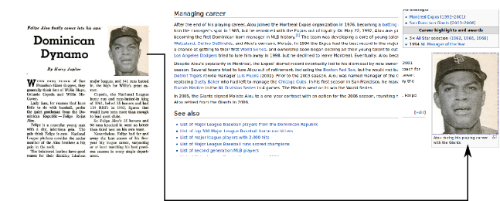
\includegraphics[scale=1]{../tables/cover_bottom.png}
\vspace{2mm}
\caption*{(2) Johnny Callison's image in January 1964 (in-copyright) issue of Baseball Digest, not reused on Wikipedia}
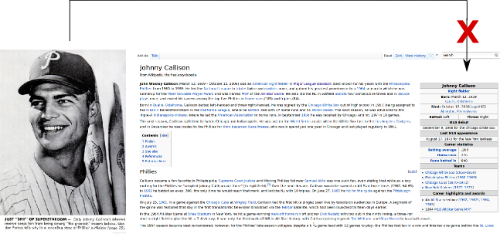
\includegraphics[scale=1]{../tables/cover_top.png}

\end{center}
\begin{quote}
\vspace{5mm}
\end{quote}
\end{figure}

%%% Fig 2: mean charts, digitization
\begin{figure}[!htbp]
\begin{center}
\caption{Citations to Baseball Digest on Wikipedia (Sample A)}
\label{fig:overview}
\caption*{(1) Citations to Baseball Digest before and after Digitization}
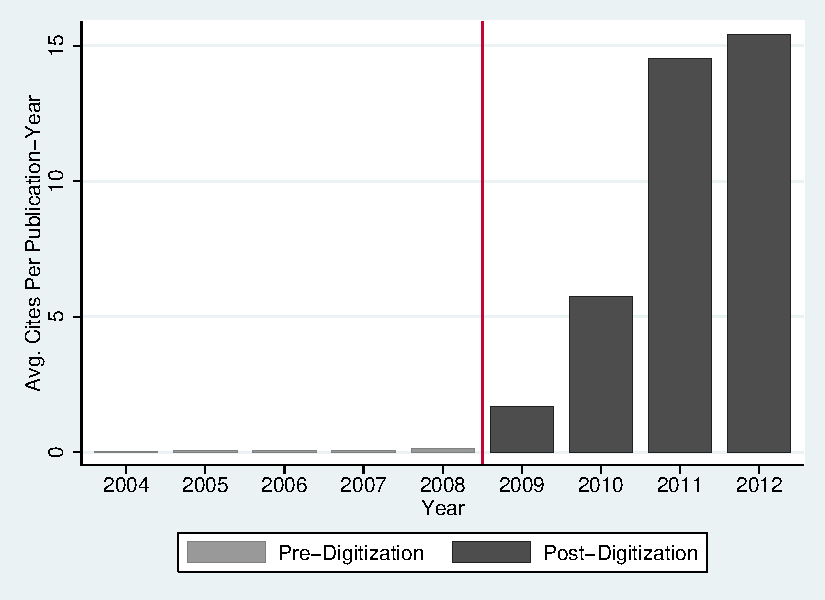
\includegraphics[scale=0.75]{../tables/mean_digit.pdf}
\vspace{5mm}
\caption*{(2) Citations to Baseball Digest for issues published before and after 1964}
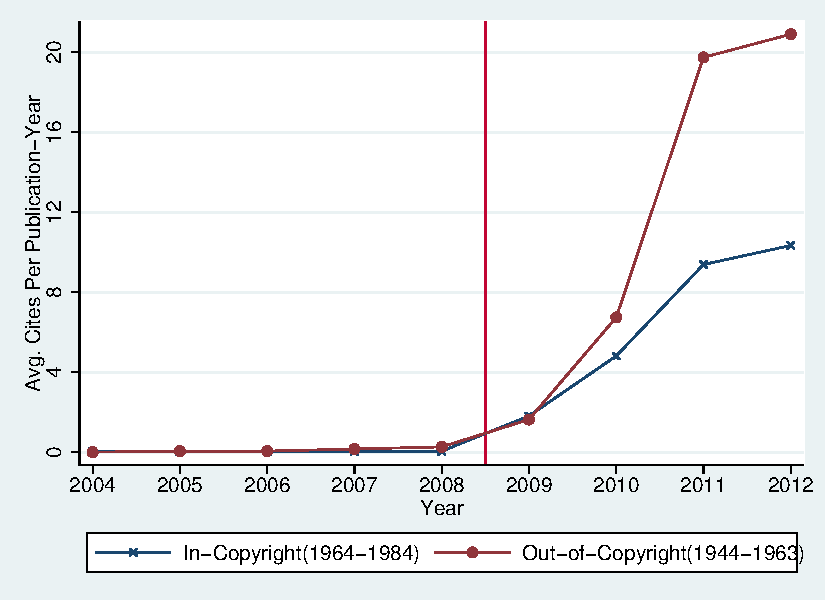
\includegraphics[scale=0.75]{../tables/mean_connected_cites.pdf}
%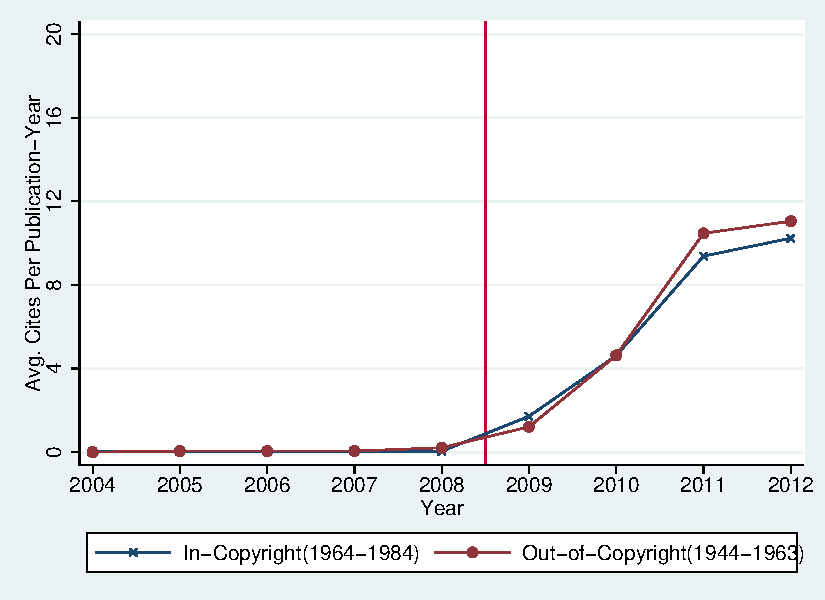
\includegraphics[scale=0.25]{../tables/mean_connected_text.pdf}
%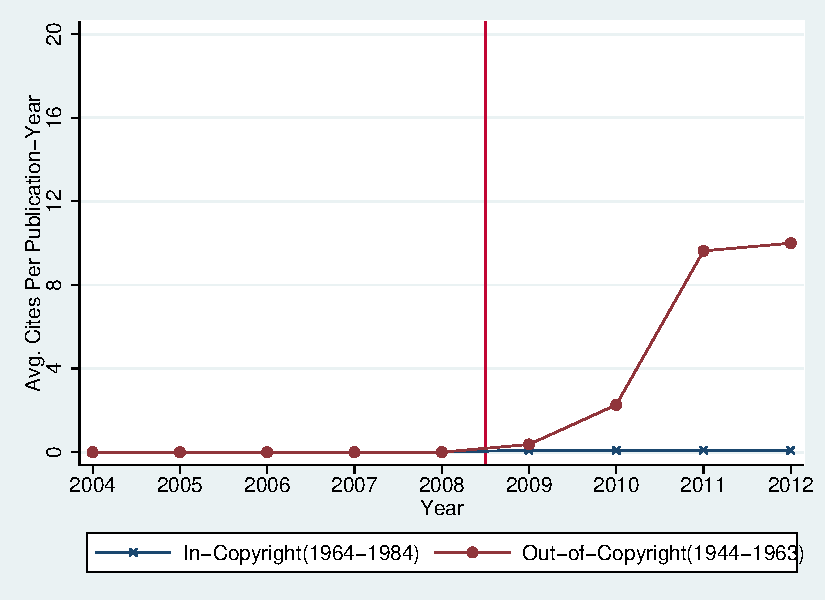
\includegraphics[scale=0.25]{../tables/mean_connected_img.pdf}
\end{center}

\begin{quote}
\emph{Note:} This plot presents some simple descriptive data on citations to Baseball Digest issues. Panel (1) presents average citations per publication-year of Baseball Digest on Wikipedia before and after the Google Books digitization event in 2008. Panel (2) presents similar information, but data are presented separately for all publication-years before 1964 (out-of-copyright) and those in or after 1964 (in-copyright). See text for more detailed data and variable descriptions. 
\end{quote}
\end{figure}

%% Fig 3. DD picture
%\begin{landscape}

\begin{figure}[!htbp]
\begin{center}
\caption{Time-Varying Estimates of the Impact of Copyright\\ on Citations to Baseball Digest}
\label{fig:ddpic}
\caption*{(1) Sample A : Total Citations}
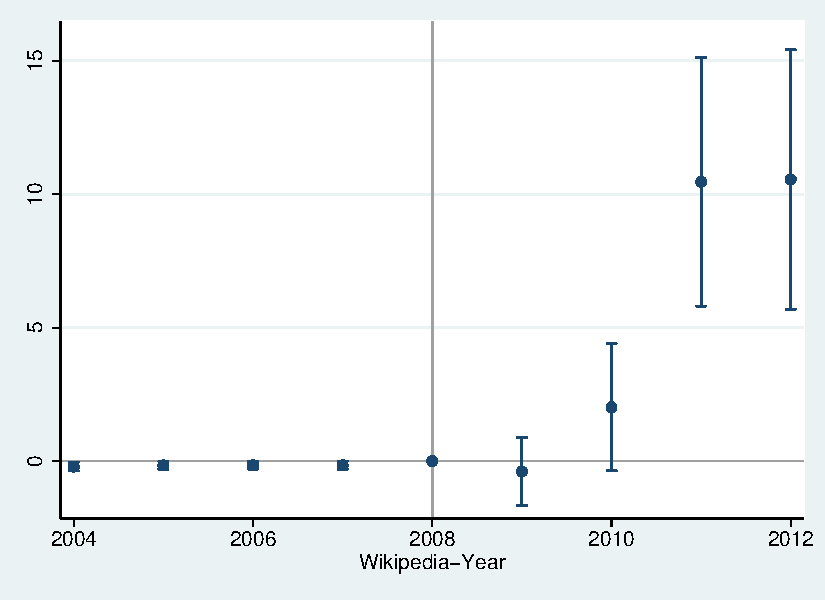
\includegraphics[scale=0.7]{../tables/cite_timeline_cites.pdf}
\vspace{2mm}
\caption*{(2) Sample B : Total Citations}
%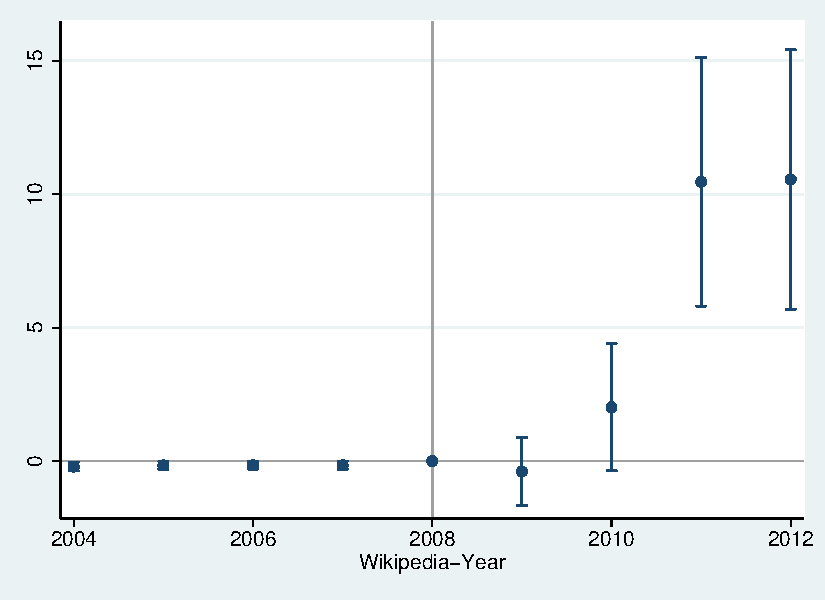
\includegraphics[scale=0.6]{../tables/cite_timeline_cites.pdf}
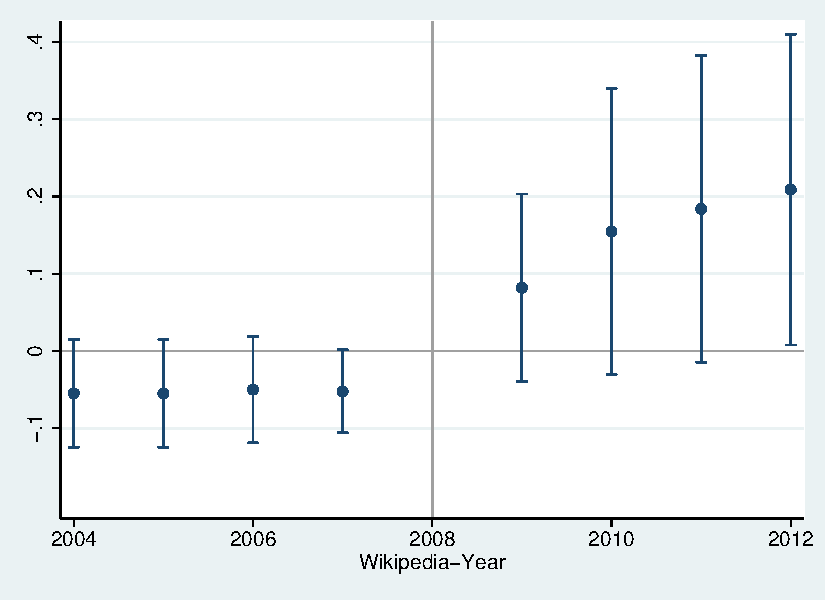
\includegraphics[scale=0.7]{../tables/timeline_bd_1.pdf}

%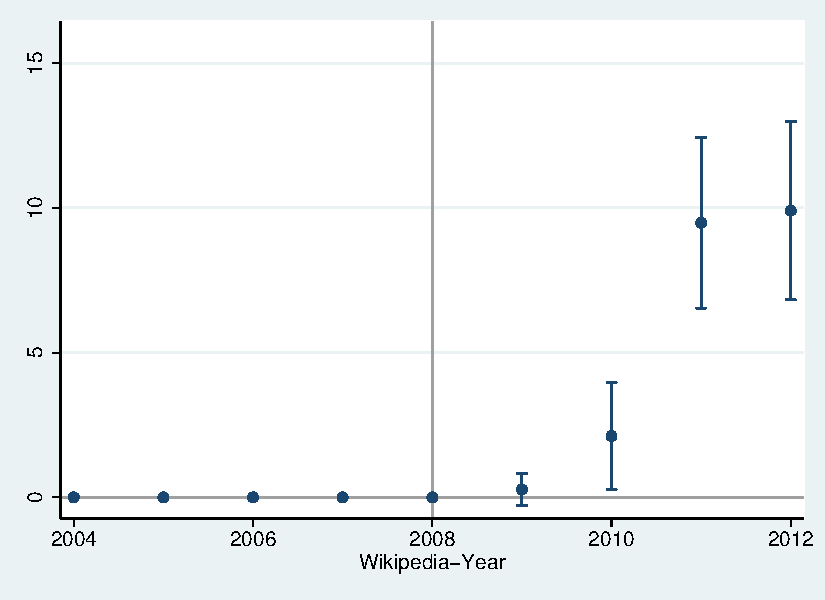
\includegraphics[scale=0.6]{../tables/cite_timeline_img.pdf}
%\vspace{5mm}
%\caption*{Panel B : Basketball Players}
%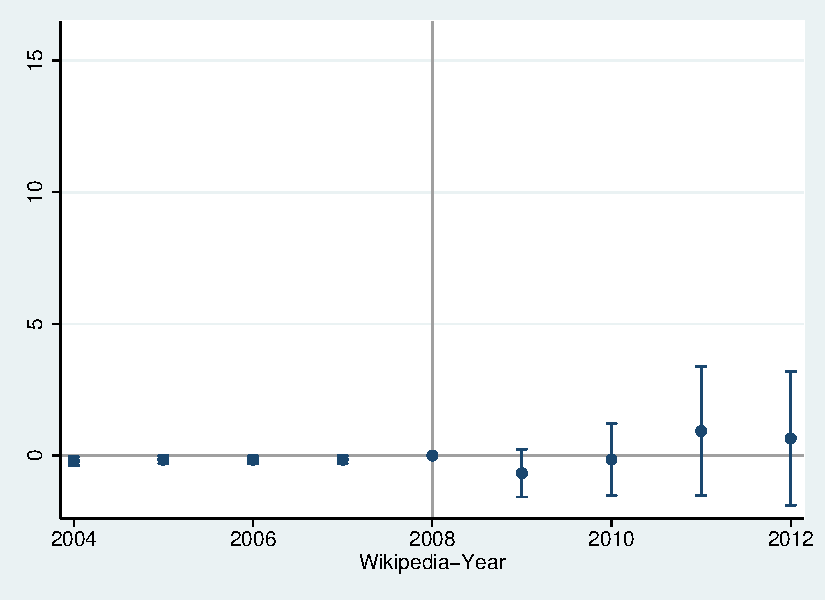
\includegraphics[scale=0.6]{../tables/cite_timeline_text.pdf}
\end{center}

\begin{quote}
%\begin{adjustwidth}{-2cm}{-2cm}
\emph{Note:} This figure plots coefficients (and 95 percent confidence intervals) from the event study specifications described in Section \ref{sec:timevary}. On the $x$ axis is the Wikipedia-year and the reference year is 2008, the year of the digitization event. This specification is based on Sample A for Panel (1) and Sample B for Panel (2), the coefficients are estimates from ordinary-least-squares (OLS) models, and standard errors are clustered. The dependent variable in both panels is the total number of citations in a calendar year. See text for more detailed data and variable descriptions. 
%\end{adjustwidth}

\end{quote}
\end{figure}
%\end{landscape}


%Fig 4. Killer Pic Sample A
%\begin{landscape}

\begin{figure}[!htbp]
\begin{center}
\caption{Citations to Baseball Digest Published Before and After the 1964 Copyright Cutoff (Sample A)}
\label{fig:killer_cite}
%\caption*{Panel A : Citation Gains at the Issue-Year Level between 2012 and 2008}
\vspace{1cm}

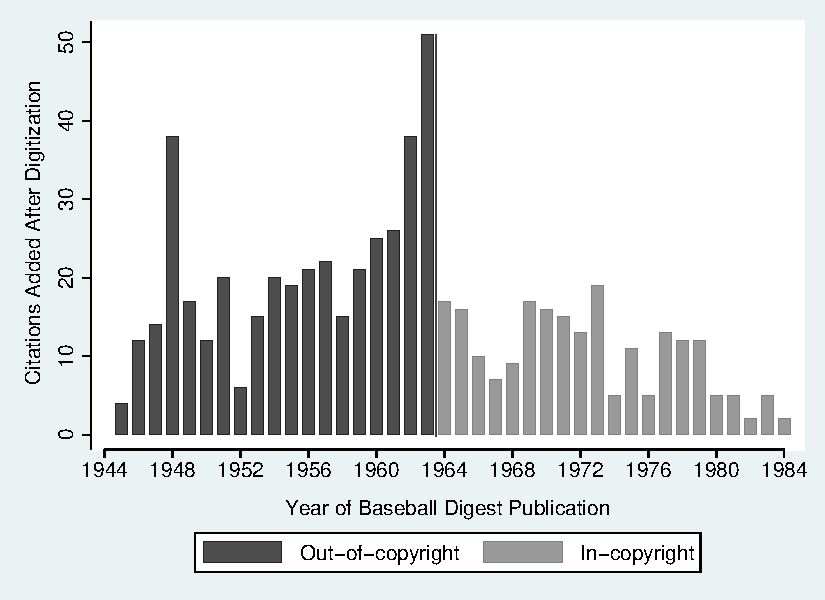
\includegraphics[scale=1]{../tables/cite_killer_cite.pdf}
%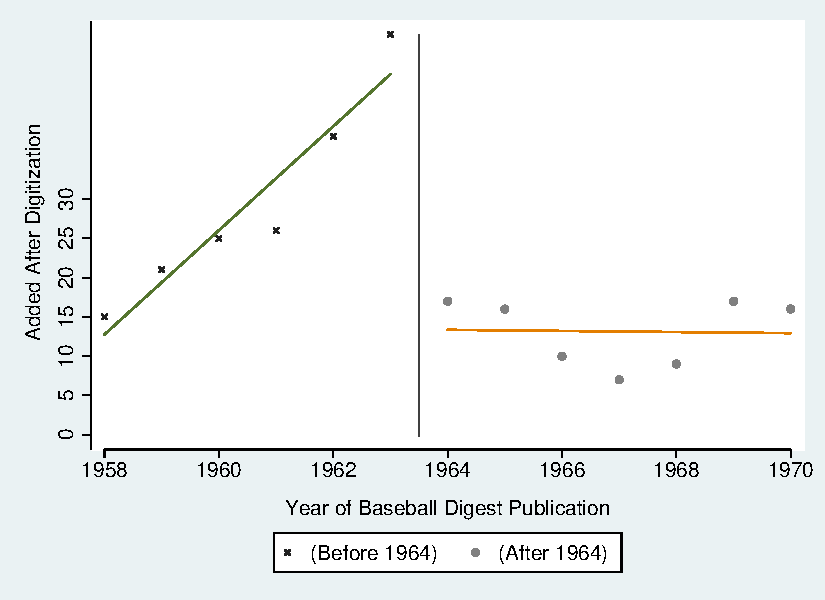
\includegraphics[scale=1]{../tables/cite_scatter_cite.pdf}


%\vspace{2mm}
%\caption*{Panel B : Comparing Citation Gains For Image Reuse and In-Text Citations}
%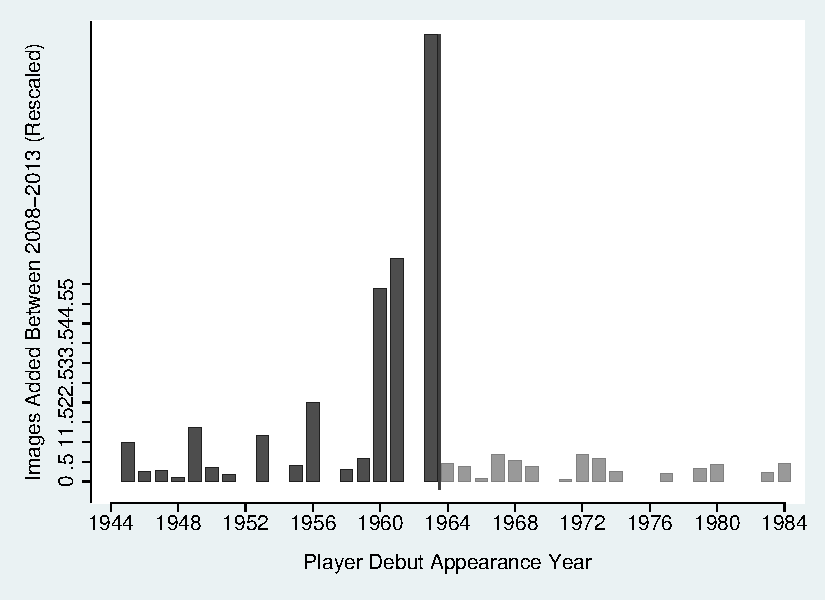
\includegraphics[scale=0.75]{../tables/killerpic2_1_bd.pdf}

%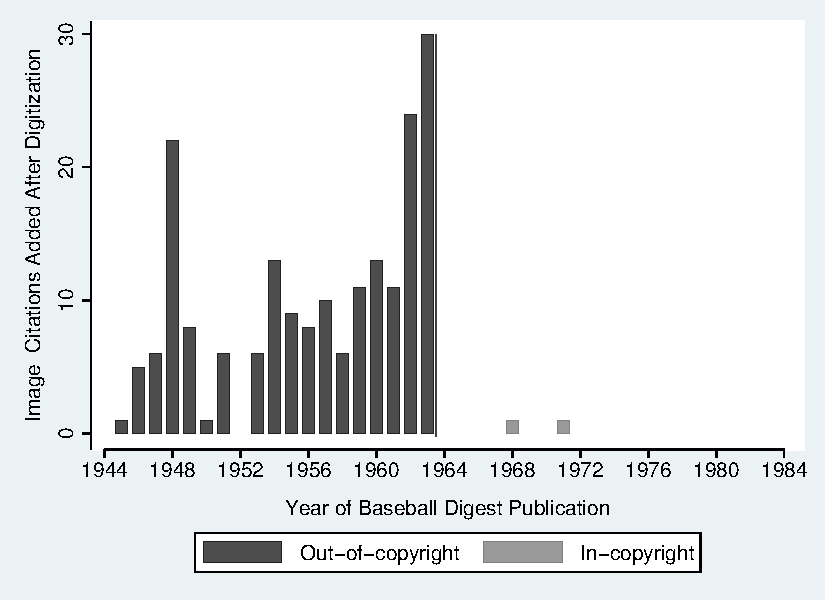
\includegraphics[scale=0.65]{../tables/cite_killer_img.pdf}
%\vspace{5mm}
%\caption*{Panel B : Basketball Players}
%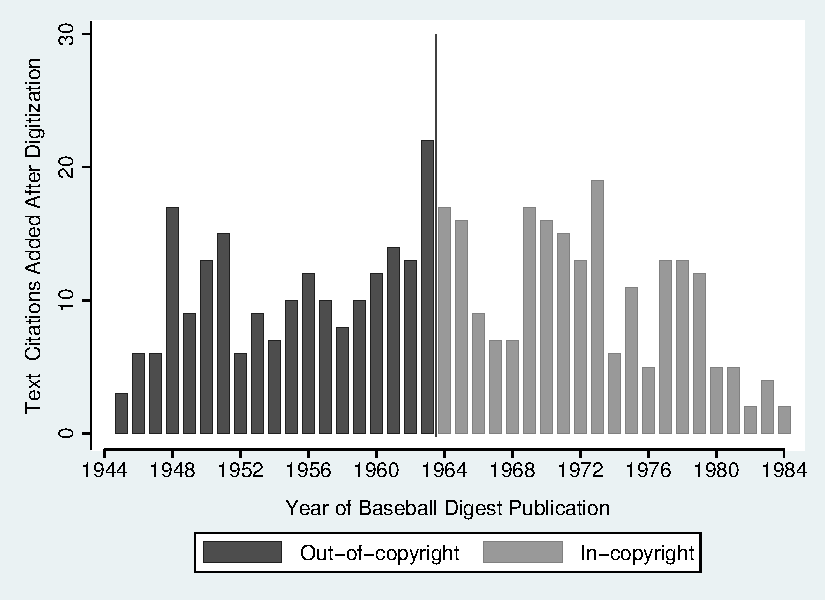
\includegraphics[scale=0.65]{../tables/cite_killer_text.pdf}
\end{center}
\vspace{1cm}
\begin{quote}
%\begin{adjustwidth}{-2cm}{-2cm}
\emph{Note:} This figure plots the growth in citations to Baseball Digest publication-years in 2012 as compared to 2008. Out-of-copyright publication-years (1944-1963) are shown in dark grey, while in-copyright publication-years (1964-1984) are shown in light grey. See text for more detailed data and variable descriptions. 
%\end{adjustwidth}

\end{quote}
\end{figure}
%\end{landscape}

\newpage


%\newpage
%%\begin{landscape}
%%%%% Fig 5. Killer Pic for Images and Text

\newpage
%\begin{landscape}

\begin{figure}[!htbp]
\begin{center}
\caption{Impact of Copyright on Image and Text Citations (Sample A)}
\label{fig:killer_img}
\caption*{(1) Image Citations}

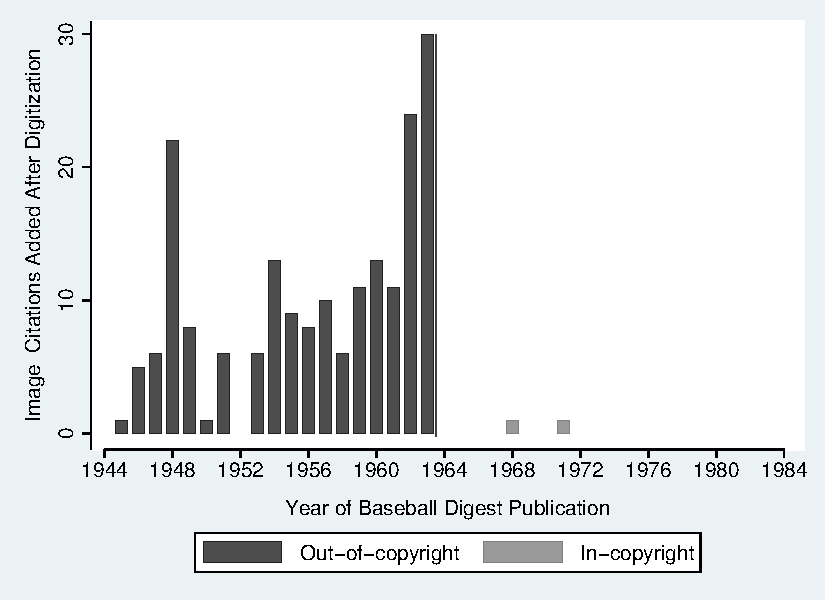
\includegraphics[scale=0.7]{../tables/cite_killer_img.pdf}

\vspace{0.2cm}
\caption*{(2) Text Citations}
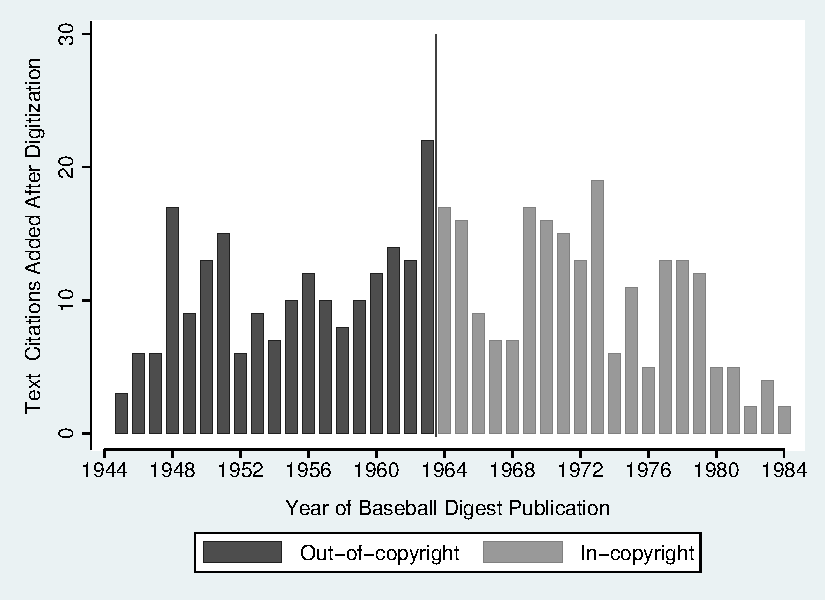
\includegraphics[scale=0.75]{../tables/cite_killer_text.pdf}

%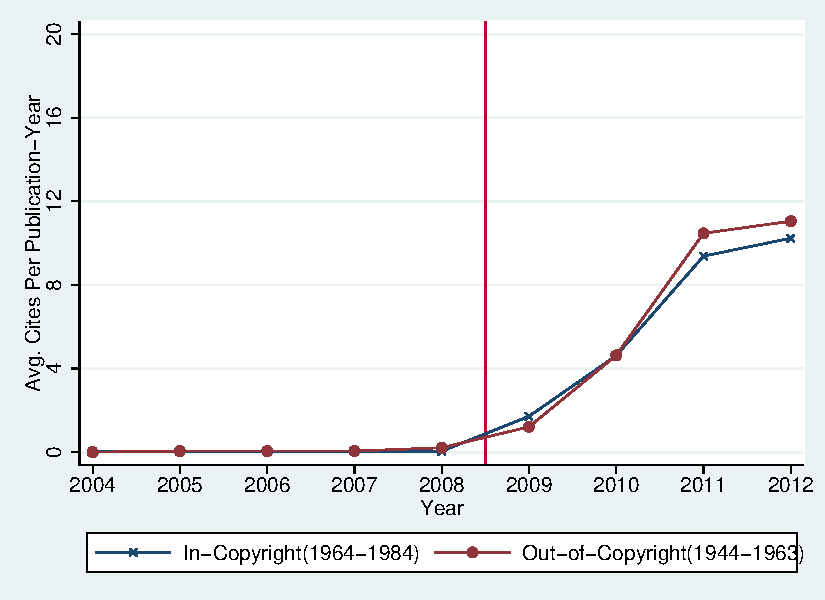
\includegraphics[scale=0.25]{../tables/mean_connected_text.pdf}
%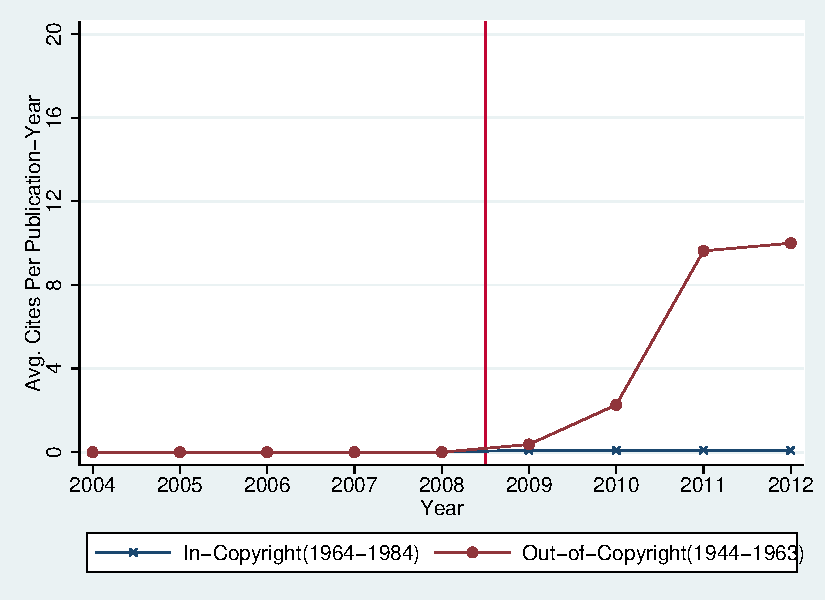
\includegraphics[scale=0.25]{../tables/mean_connected_img.pdf}
\vspace{5mm}

%\caption*{Panel B : Time Varying Estimates of the Impact of Copyright on Wikipedia Pages}
%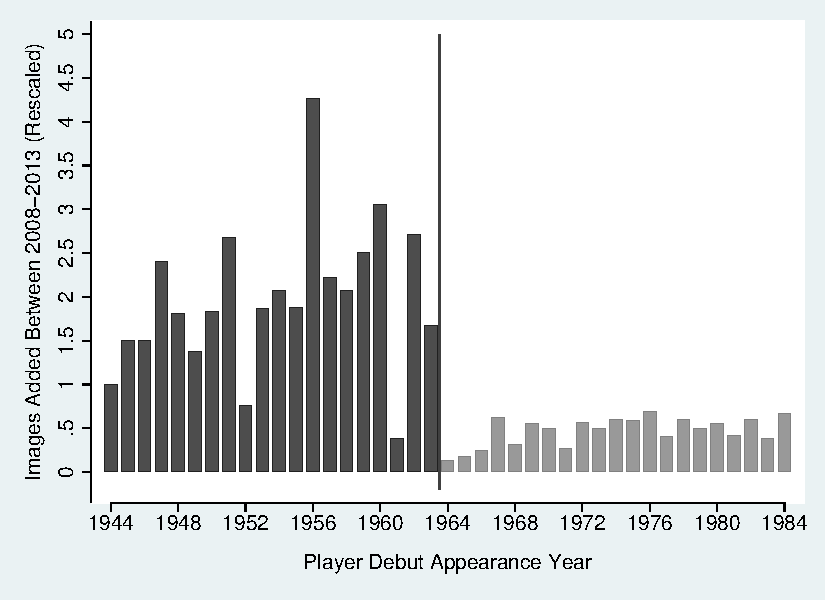
\includegraphics[scale=0.65]{../tables/killerpic2_1_img.pdf}
%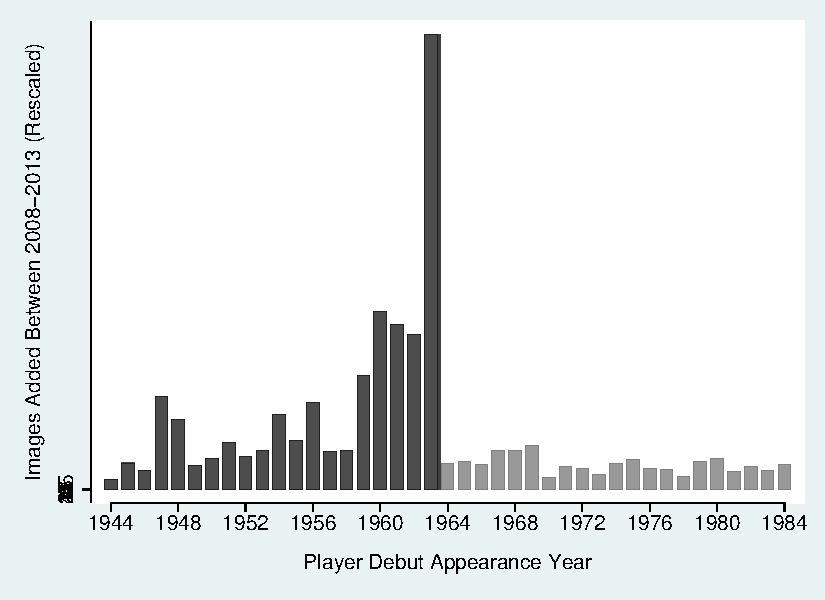
\includegraphics[scale=0.65]{../tables/killerpic2_1_text.pdf}
%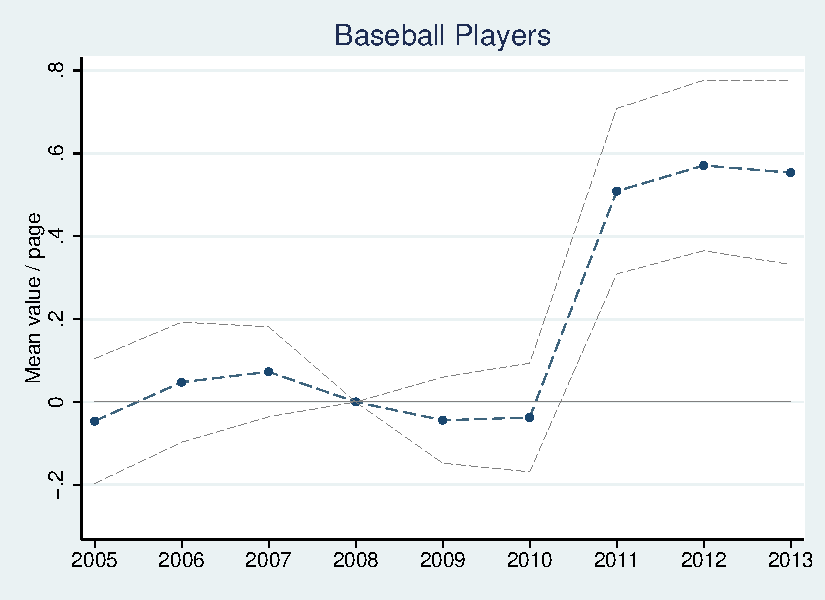
\includegraphics[scale=0.75]{../tables/timeline_img_1.pdf}
%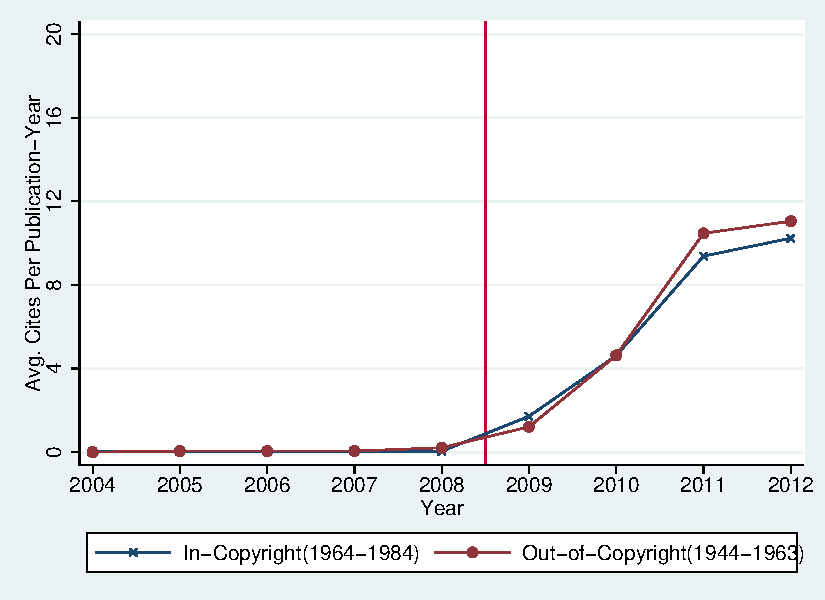
\includegraphics[scale=0.25]{../tables/mean_connected_text.pdf}
%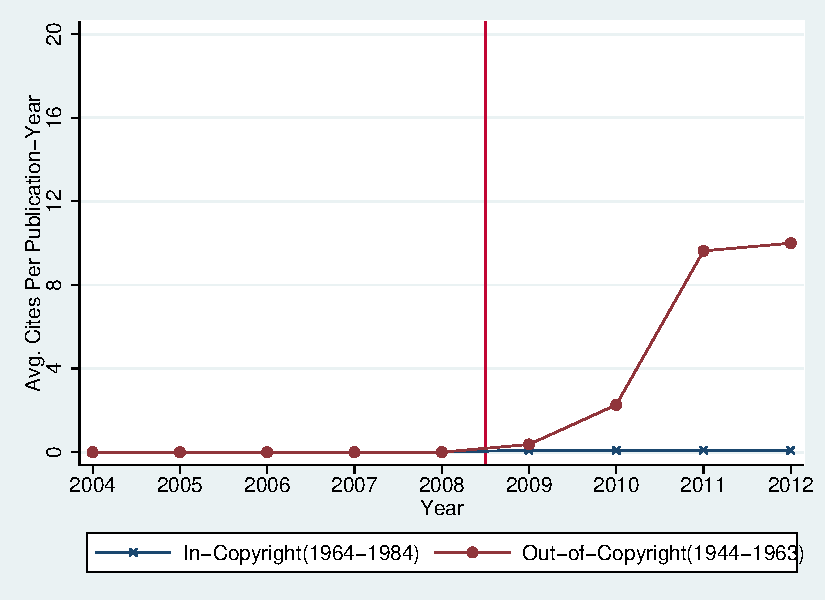
\includegraphics[scale=0.25]{../tables/mean_connected_img.pdf}
\end{center}

\begin{quote}
%\begin{adjustwidth}{-2cm}{-2cm}
%\emph{Note:} This chart documents the impact of the 1964 copyright cutoff for Baseball Digest on the reuse of images and text

\emph{Note:} This figure plots the growth in citations to Baseball Digest publication-years in 2012 as compared to 2008. Panel (1) plots the growth in Image citations, while Panel (2) plots the growth in Text citations. Out-of-copyright publication-years (1944-1963) are shown in dark grey, while in-copyright publication-years (1964-1984) are shown in light grey. See text for more detailed data and variable descriptions. 


%number of images added to baseball Wikipedia pages. Panel A documents the variation in the number of images added between 2008 and 2013 for out-of-copyright (debut before 1964) players and in-copyright (debut after 1964) players. The raw mean is adjusted to account for each player's differing exposure to the copyright rule. Panel B plots coefficients (and 95 percent confidence intervals) from the event study specifications described in Section \ref{sec:timevary}. On the $x$ axis is the calendar year and the reference year is 2008, the year of the digitization event. This specification is based on page-year level observations, the coefficients are estimates from ordinary-least-squares (OLS) models, and standard errors are clustered at the page level. See text for more detailed data and variable descriptions. 
%\end{adjustwidth}
\end{quote}
\end{figure}

%\end{landscape}

%%%%%%%%%%%
%%%%% Fig 6. DD Pic 2 for Images and Text
%%%%%%%%%%%

\begin{figure}[!htbp]
\begin{center}
\caption{Time-Varying Estimates for Image and Text Citations (Sample A)}
\label{fig:ddpic_img}
\caption*{\small{(1) Image Citations}}
%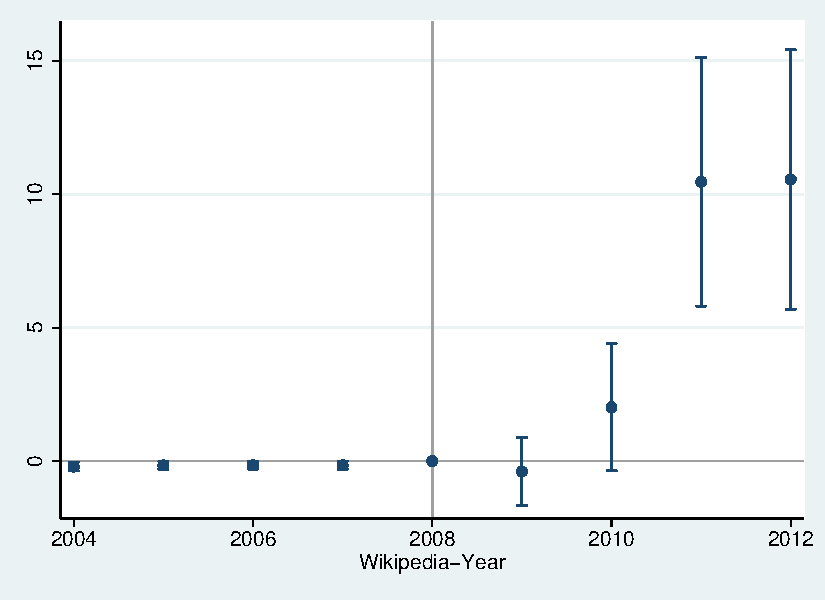
\includegraphics[scale=0.75]{../tables/cite_timeline_cites.pdf}
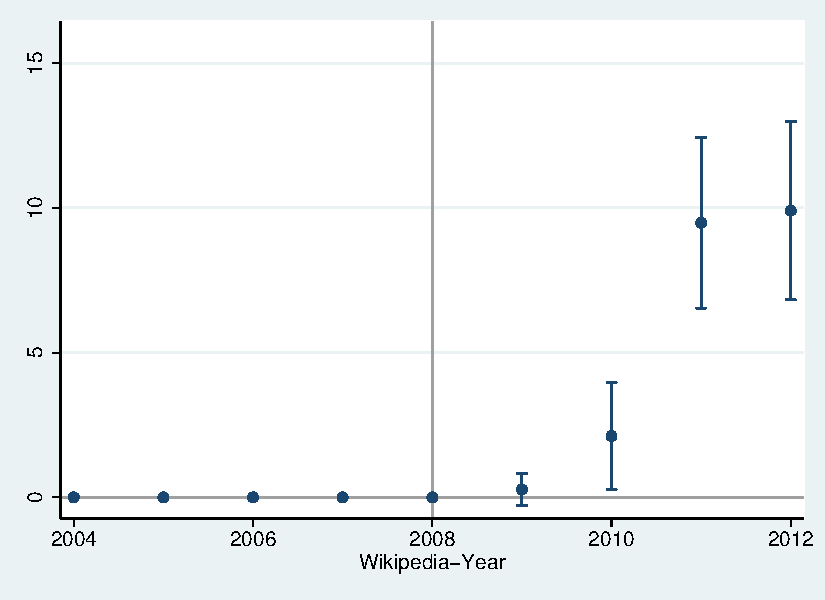
\includegraphics[scale=0.75]{../tables/cite_timeline_img.pdf}

\caption*{\small{(2) Text Citations}}
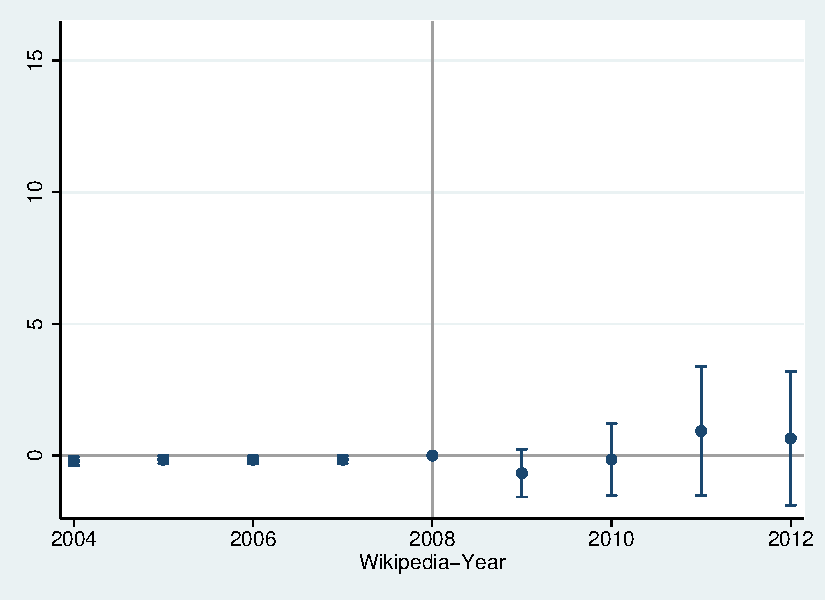
\includegraphics[scale=0.75]{../tables/cite_timeline_text.pdf}
\vspace{2mm}

%\caption*{Sample B : }
%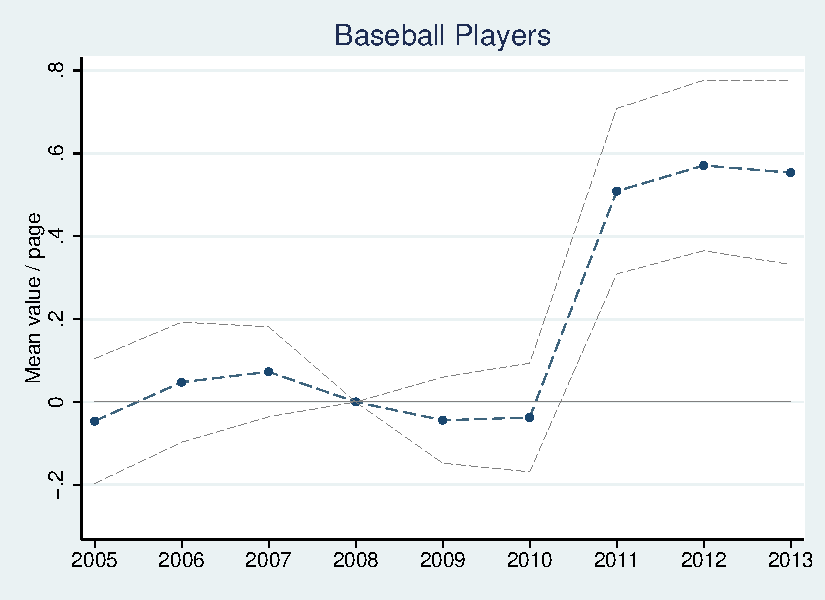
\includegraphics[scale=0.6]{../tables/timeline_img_1.pdf}
%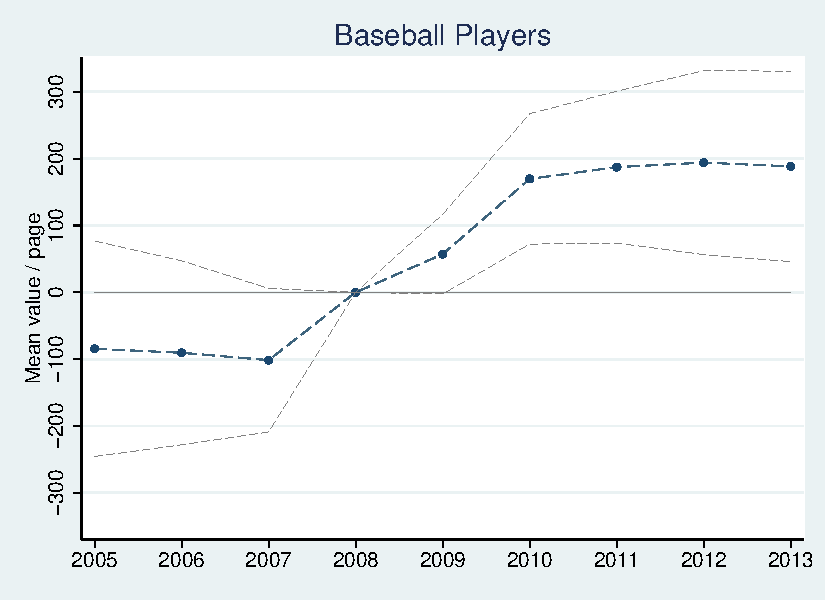
\includegraphics[scale=0.6]{../tables/timeline_text_1.pdf}

%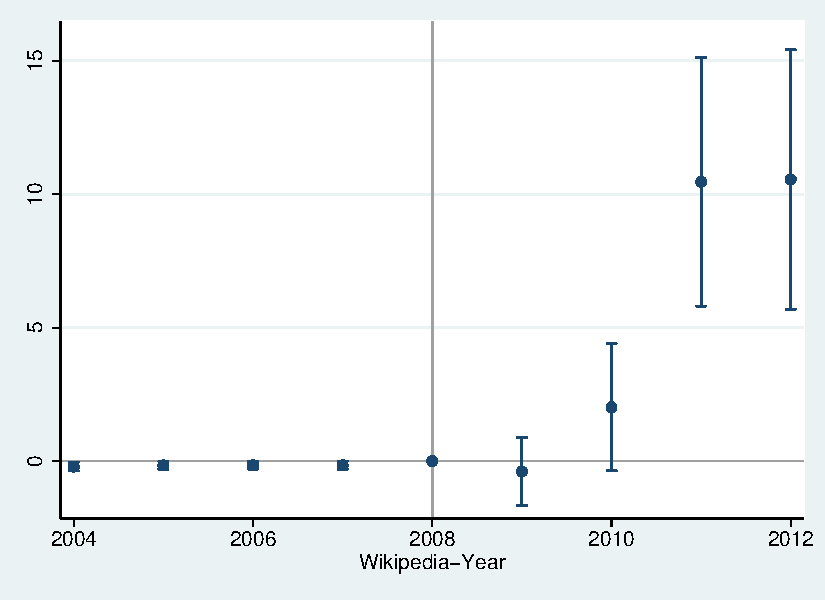
\includegraphics[scale=0.6]{../tables/cite_timeline_cites.pdf}

%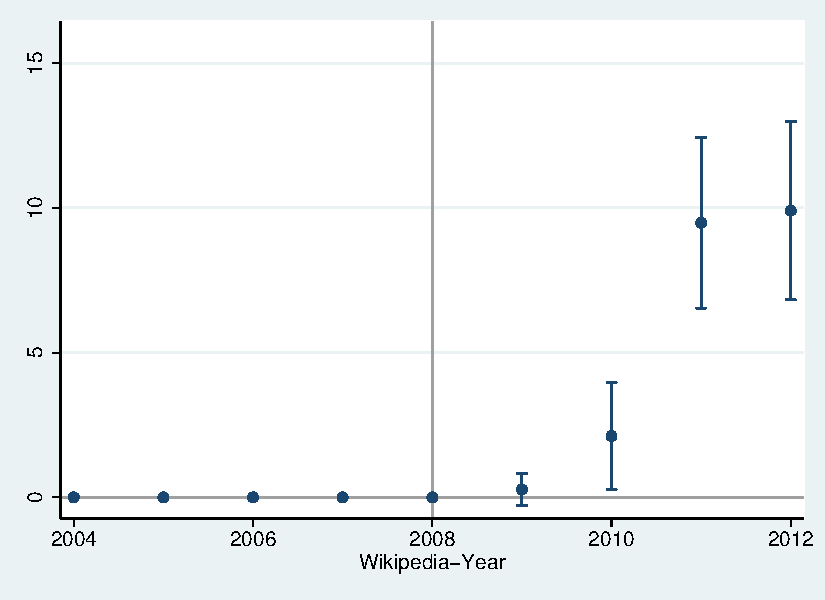
\includegraphics[scale=0.6]{../tables/cite_timeline_img.pdf}
%\vspace{5mm}
%\caption*{Panel B : Basketball Players}
%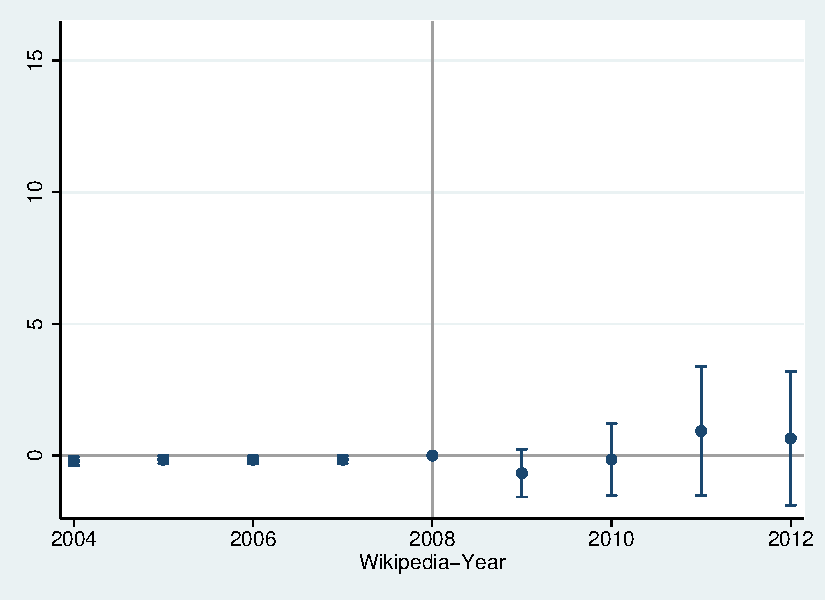
\includegraphics[scale=0.6]{../tables/cite_timeline_text.pdf}
\end{center}

\begin{quote}
\emph{Note:} This figure plots coefficients (and 95 percent confidence intervals) from the event study specifications described in Section \ref{sec:timevary} separately for image (Panel 1) and text citations (Panel 2). On the $x$ axis is the Wikipedia-year and the reference year is 2008, the year of the digitization event. This specification is based on Sample A for Panel (1) and (2). The coefficients are estimated from ordinary-least-squares (OLS) models, and standard errors are clustered. The dependent variable in both panels is the total number of citations in a calendar year. See text for more detailed data and variable descriptions. 

\end{quote}
\end{figure}



%%%%%%%%%%%
%%% Fig 7: HETERO EFFECTS
%%%%%%%%%%%

\begin{figure}[!htbp]
\begin{center}
\caption{Heterogeneous Impacts of Copyright on Wikipedia Pages by Player Quality (Sample B)}
\label{fig:quality}
\vspace{5mm}
\caption*{\small{(1) Images}}
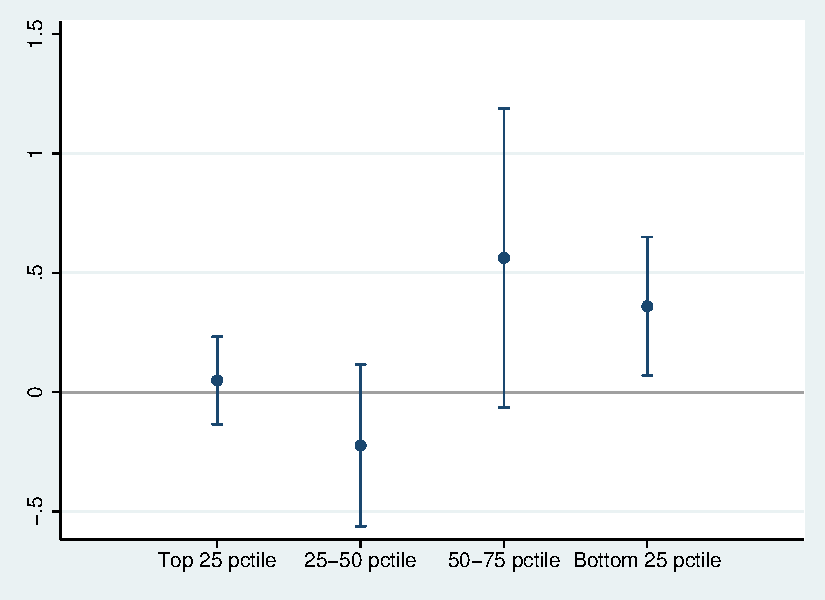
\includegraphics[scale=0.70]{../tables/quality_img.pdf}\\
\vspace{5mm}
\caption*{\small{(2) Traffic}}
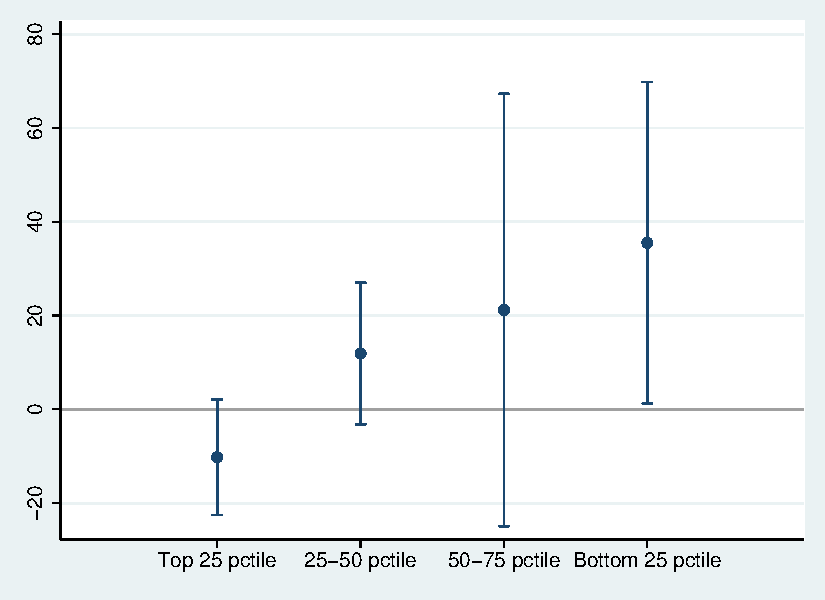
\includegraphics[scale=0.70]{../tables/quality_traf.pdf}

\end{center}
\begin{quote}
%\begin{adjustwidth}{-2cm}{-2cm}
\emph{Note:} This plot documents the differential impact of the Baseball Digest copyright cutoff on baseball player pages of different \emph{quality} as described in Section \ref{sec:diff2}. For this analysis, players are split into 4 different levels of quality based on their percentile rank within the sample of baseball players and the main difference-in-difference estimates are calculated separately for each of the four quality percentiles. Panel (1) plots these estimates for Image Citations, while Panel (2) plots estimates for Traffic. See text for detailed data and variable descriptions.

%%Coefficients ($\beta_3$) are derived from the specification: 

%%$Y_{it} = \alpha + \beta_1 \times post_t \times out-of-copy_i + \beta_2 \times post_t \times quality_i + \beta_3 \times post_t \times out-of-copy_i \times quality_i + \gamma_i+ \delta_t + \epsilon_{it}$ 

%%where $\gamma_{i}$ and $\delta_{t}$ represents player and time fixed effects respectively for player $i$ and year $t$.  All estimates are from ordinary-least-squares (OLS) models. 

%\end{adjustwidth}
\end{quote}
\end{figure}

%%\end{landscape}

%%%%%%%%%%%%%%%% APPENDIX %%%%%%%%%%%%%%%%%%%%%%%%%%%
%blank
%\newpage
%\newpage

\appendix

\setcounter{table}{0}\renewcommand{\thetable}{A.\arabic{table}}
\setcounter{figure}{0}\renewcommand{\thefigure}{A.\arabic{figure}}

%%%%% DD Table %%%%
\begin{center}
\begin{table}[!htbp]
\section{Appendices}

\subsection{Appendix A1 : Robustness Checks}
\label{sec:envelope}

%% BASKETBALL DATA Added

\caption{Estimating the Causal Impact of Digitization}
\vspace{5mm}
{
\def\sym#1{\ifmmode^{#1}\else\(^{#1}\)\fi}
\begin{tabular*}{\hsize}{@{\hskip\tabcolsep\extracolsep\fill}l*{3}{c}}
\toprule
            &\multicolumn{3}{c}{Digitization DD}                              \\\cmidrule(lr){2-4}
            &\multicolumn{1}{c}{Citations}&\multicolumn{1}{c}{Images}&\multicolumn{1}{c}{Text}\\
\midrule
\emph{baseball X post}&       0.340         &       0.459         &       0.391         \\
            &    (0.0494)\sym{***}&    (0.0610)\sym{***}&    (0.0650)\sym{***}\\
\midrule
Player FE   &         Yes         &         Yes         &         Yes         \\
Time FE     &        Year         &        Year         &        Year         \\
adj. $R^2$  &      0.0687         &       0.172         &       0.399         \\
N           &       13260         &       13260         &       13260         \\
Clusters    &        1105         &        1105         &        1105         \\
\bottomrule
\end{tabular*}
}

\begin{quote}
\vspace{5mm}

\emph{+:p$<$0.15; *:p$<$0.10; **:p$<$0.05; ***:p$<$0.01 
\newline
Standard errors clustered at player-level shown in parentheses.}

\vspace{5mm}

\emph{Note:} This table provides estimates that help to determine the causal impact of the Google Books digitization event on reuse. I supplement data in Sample B, with similar data from Wikipedia player-pages for a comparable set of 564 basketball players. The estimates are provided from a difference-in-difference specification where the treatment group is the set of baseball player-pages and the post-period are the years 2009-2012 after the digitization event. All estimates are from ordinary-least-squares (OLS) models. See text for detailed data and variable descriptions.
\end{quote}
\label{tab:basketball}
\end{table}
\end{center}



%%% LEADS - LAGS
\begin{center}
\begin{table}[!htbp]

\caption{Robustness: Exploring pre-trends between in-copyright and out-of-copyright Issues}
%\vspace{5mm}
{\small
{
\def\sym#1{\ifmmode^{#1}\else\(^{#1}\)\fi}
\begin{tabular*}{\hsize}{@{\hskip\tabcolsep\extracolsep\fill}l*{6}{c}}
\toprule
            &\multicolumn{3}{c}{Sample A}                                     &\multicolumn{3}{c}{Sample B}                                     \\\cmidrule(lr){2-4}\cmidrule(lr){5-7}
            &\multicolumn{1}{c}{Citations}&\multicolumn{1}{c}{Images}&\multicolumn{1}{c}{Text}&\multicolumn{1}{c}{Citations}&\multicolumn{1}{c}{Images}&\multicolumn{1}{c}{Text}\\
\midrule
$Digitization_{-3}$&      -0.000         &      -0.000         &      -0.000         &      -0.008         &      -0.194         &      -0.642         \\
            &         (.)         &     (0.000)         &     (0.000)         &     (0.004)\sym{*}  &     (0.024)\sym{***}&     (0.031)\sym{***}\\
\addlinespace
$Digitization_{-2}$&      -0.000         &      -0.000         &      -0.000         &      -0.008         &      -0.075         &      -0.359         \\
            &         (.)         &     (0.000)         &     (0.000)         &     (0.004)\sym{**} &     (0.027)\sym{***}&     (0.022)\sym{***}\\
\addlinespace
$Digitization_{-1}$&      -0.000         &      -0.000         &      -0.000         &      -0.003         &      -0.033         &      -0.106         \\
            &     (0.000)         &     (0.000)         &     (0.000)         &     (0.003)         &     (0.019)\sym{*}  &     (0.009)\sym{***}\\
\addlinespace
$Digitization_{+1}$&       1.762         &       0.095         &       1.667         &       0.046         &       0.060         &       0.088         \\
            &     (0.424)\sym{***}&     (0.066)         &     (0.421)\sym{***}&     (0.015)\sym{***}&     (0.016)\sym{***}&     (0.007)\sym{***}\\
\addlinespace
$Digitization_{+2}$&       4.762         &       0.095         &       4.667         &       0.112         &       0.140         &       0.220         \\
            &     (0.680)\sym{***}&     (0.066)         &     (0.681)\sym{***}&     (0.027)\sym{***}&     (0.020)\sym{***}&     (0.012)\sym{***}\\
\addlinespace
$Digitization_{+3}$&       9.333         &       0.095         &       9.238         &       0.128         &       0.220         &       0.397         \\
            &     (1.064)\sym{***}&     (0.066)         &     (1.060)\sym{***}&     (0.028)\sym{***}&     (0.026)\sym{***}&     (0.017)\sym{***}\\
\addlinespace
$Digitization_{+4}$&      10.286         &       0.095         &      10.190         &       0.132         &       0.259         &       0.472         \\
            &     (1.195)\sym{***}&     (0.066)         &     (1.189)\sym{***}&     (0.028)\sym{***}&     (0.026)\sym{***}&     (0.020)\sym{***}\\
\addlinespace
$Digitization_{-3}$ x out-of-copy&      -0.211         &       0.000         &      -0.211         &      -0.040         &      -0.093         &      -0.180         \\
            &     (0.097)\sym{**} &     (0.000)         &     (0.097)\sym{**} &     (0.027)\sym{+}  &     (0.064)\sym{+}  &     (0.084)\sym{**} \\
\addlinespace
$Digitization_{-2}$ x out-of-copy&      -0.211         &       0.000         &      -0.211         &      -0.037         &      -0.013         &      -0.127         \\
            &     (0.097)\sym{**} &     (0.000)         &     (0.097)\sym{**} &     (0.027)         &     (0.062)         &     (0.067)\sym{*}  \\
\addlinespace
$Digitization_{-1}$ x out-of-copy&      -0.105         &       0.000         &      -0.105         &      -0.035         &       0.033         &      -0.114         \\
            &     (0.073)         &     (0.000)         &     (0.073)         &     (0.021)\sym{*}  &     (0.052)         &     (0.050)\sym{**} \\
\addlinespace
$Digitization_{+1}$ x out-of-copy&      -0.393         &       0.273         &      -0.667         &       0.077         &      -0.038         &       0.050         \\
            &     (0.757)         &     (0.327)         &     (0.544)         &     (0.045)\sym{*}  &     (0.042)         &     (0.024)\sym{**} \\
\addlinespace
$Digitization_{+2}$ x out-of-copy&       1.712         &       2.115         &      -0.404         &       0.160         &      -0.013         &       0.124         \\
            &     (1.443)         &     (1.100)\sym{*}  &     (0.834)         &     (0.068)\sym{**} &     (0.055)         &     (0.039)\sym{***}\\
\addlinespace
$Digitization_{+3}$ x out-of-copy&      10.140         &       9.484         &       0.657         &       0.187         &       0.383         &       0.101         \\
            &     (2.762)\sym{***}&     (1.748)\sym{***}&     (1.453)         &     (0.073)\sym{**} &     (0.083)\sym{***}&     (0.046)\sym{**} \\
\addlinespace
$Digitization_{+4}$ x out-of-copy&      10.346         &       9.905         &       0.441         &       0.206         &       0.454         &       0.117         \\
            &     (2.938)\sym{***}&     (1.826)\sym{***}&     (1.581)         &     (0.074)\sym{***}&     (0.086)\sym{***}&     (0.055)\sym{**} \\
\midrule
Player FE   &         Yes         &         Yes         &         Yes         &         Yes         &         Yes         &         Yes         \\
Time FE     &        Year         &        Year         &        Year         &        Year         &        Year         &        Year         \\
adj. $R^2$  &       0.748         &       0.573         &       0.799         &       0.043         &       0.134         &       0.365         \\
N           &     360.000         &     360.000         &     360.000         &    9945.000         &    9945.000         &    9945.000         \\
\bottomrule
\end{tabular*}
}

}
\begin{quote}
\vspace{5mm}

\emph{+:p$<$0.15; *:p$<$0.10; **:p$<$0.05; ***:p$<$0.01 
\newline
Standard errors clustered at player-level shown in parentheses.}

\vspace{5mm}

%\emph{Note:} This table presents XXX
\end{quote}
\label{tab:leads_lags}
\end{table}
\end{center}

%%% Falsitifction
\begin{center}
\begin{table}[!htbp]

\caption{Falsification Check -- Alternate Treatment Years}
\vspace{5mm}
%{
\def\sym#1{\ifmmode^{#1}\else\(^{#1}\)\fi}
\begin{tabular*}{\hsize}{@{\hskip\tabcolsep\extracolsep\fill}l*{6}{c}}
\toprule
            &\multicolumn{3}{c}{Sample A}                                     &\multicolumn{3}{c}{Sample B}                                     \\\cmidrule(lr){2-4}\cmidrule(lr){5-7}
            &\multicolumn{1}{c}{Citations}&\multicolumn{1}{c}{Images}&\multicolumn{1}{c}{Text}&\multicolumn{1}{c}{Citations}&\multicolumn{1}{c}{Images}&\multicolumn{1}{c}{Text}\\
\midrule
\emph{out-of-copy X post}&    -0.00835         &      0.0911         &     -0.0994         &      0.0631         &      0.0631         &      0.0631         \\
            &     (0.266)         &     (0.108)         &     (0.195)         &    (0.0398)         &    (0.0398)         &    (0.0398)         \\
\midrule
Player FE   &         Yes         &         Yes         &         Yes         &         Yes         &         Yes         &         Yes         \\
Time FE     &        Year         &        Year         &        Year         &        Year         &        Year         &        Year         \\
adj. $R^2$  &       0.320         &      0.0314         &       0.385         &      0.0350         &      0.0350         &      0.0350         \\
N           &         240         &         240         &         240         &        3246         &        3246         &        3246         \\
\bottomrule
\end{tabular*}
}

{
\def\sym#1{\ifmmode^{#1}\else\(^{#1}\)\fi}
\begin{tabular*}{\hsize}{@{\hskip\tabcolsep\extracolsep\fill}l*{6}{c}}
\toprule
            &\multicolumn{3}{c}{Sample A}                                     &\multicolumn{3}{c}{Sample B}                                     \\\cmidrule(lr){2-4}\cmidrule(lr){5-7}
            &\multicolumn{1}{c}{Cites}&\multicolumn{1}{c}{Cites}&\multicolumn{1}{c}{Log-Cites}&\multicolumn{1}{c}{Cites}&\multicolumn{1}{c}{Cites}&\multicolumn{1}{c}{Log-Cites}\\
\midrule
\emph{out-of-copy X post}&     -0.0209         &    -0.00835         &     -0.0105         &      0.0685         &      0.0631         &      0.0207         \\
            &     (0.296)         &     (0.266)         &    (0.0768)         &    (0.0323)\sym{**} &    (0.0398)         &    (0.0145)         \\
\midrule
Unit of Obs. FE&          No         &         Yes         &         Yes         &          No         &         Yes         &         Yes         \\
Year FE     &         Yes         &         Yes         &         Yes         &         Yes         &         Yes         &         Yes         \\
adj. $R^2$  &       0.256         &       0.320         &       0.541         &      0.0265         &      0.0350         &      0.0441         \\
N           &         240         &         240         &         240         &        3246         &        3246         &        3246         \\
\bottomrule
\end{tabular*}
}

\begin{quote}
\vspace{5mm}

\emph{+:p$<$0.15; *:p$<$0.10; **:p$<$0.05; ***:p$<$0.01 
\newline
Standard errors clustered at player-level shown in parentheses.}

\vspace{5mm}

\emph{Note:} This table presents a falsification check of the baseline specification. In this regression, the panel is restricted to years 2004 to 2009, and the treatment year is assumed to be 2007 rather than 2009. The $out-of-copy$ variable is defined as before, and unit-of-observation fixed effects and time fixed effects are included as indicated. Please see text for detailed data and variable descriptions. 
\end{quote}
\label{tab:false}
\end{table}
\end{center}

%%%%% alternate years

%%% Falsitifction
\begin{center}
\begin{table}[!htbp]

\caption{Robustness Check : Adding Panel Restrictions}
\vspace{5mm}
\caption*{(1) Wikipedia-Years 2005-2011}
%{
\def\sym#1{\ifmmode^{#1}\else\(^{#1}\)\fi}
\begin{tabular*}{\hsize}{@{\hskip\tabcolsep\extracolsep\fill}l*{6}{c}}
\toprule
            &\multicolumn{3}{c}{Sample A}                                     &\multicolumn{3}{c}{Sample B}                                     \\\cmidrule(lr){2-4}\cmidrule(lr){5-7}
            &\multicolumn{1}{c}{Citations}&\multicolumn{1}{c}{Images}&\multicolumn{1}{c}{Text}&\multicolumn{1}{c}{Citations}&\multicolumn{1}{c}{Images}&\multicolumn{1}{c}{Text}\\
\midrule
\emph{out-of-copy X post}&       4.148         &       3.992         &       0.156         &       0.180         &       0.180         &       0.180         \\
            &     (1.455)\sym{***}&     (0.884)\sym{***}&     (0.858)         &     (0.102)\sym{*}  &     (0.102)\sym{*}  &     (0.102)\sym{*}  \\
\midrule
Player FE   &         Yes         &         Yes         &         Yes         &         Yes         &         Yes         &         Yes         \\
Time FE     &        Year         &        Year         &        Year         &        Year         &        Year         &        Year         \\
adj. $R^2$  &       0.685         &       0.363         &       0.797         &      0.0695         &      0.0695         &      0.0695         \\
N           &         280         &         280         &         280         &        3787         &        3787         &        3787         \\
\bottomrule
\end{tabular*}
}

{
\def\sym#1{\ifmmode^{#1}\else\(^{#1}\)\fi}
\begin{tabular*}{\hsize}{@{\hskip\tabcolsep\extracolsep\fill}l*{6}{c}}
\toprule
            &\multicolumn{3}{c}{Sample A}                                     &\multicolumn{3}{c}{Sample B}                                     \\\cmidrule(lr){2-4}\cmidrule(lr){5-7}
            &\multicolumn{1}{c}{Cites}&\multicolumn{1}{c}{Cites}&\multicolumn{1}{c}{Log-Cites}&\multicolumn{1}{c}{Cites}&\multicolumn{1}{c}{Cites}&\multicolumn{1}{c}{Log-Cites}\\
\midrule
\emph{out-of-copy X post}&       4.035         &       3.951         &       0.198         &       0.199         &       0.180         &      0.0655         \\
            &     (1.487)\sym{***}&     (1.459)\sym{***}&     (0.150)         &    (0.0657)\sym{***}&     (0.102)\sym{*}  &    (0.0345)\sym{*}  \\
\midrule
Unit of Obs. FE&          No         &         Yes         &         Yes         &          No         &         Yes         &         Yes         \\
Year FE     &         Yes         &         Yes         &         Yes         &         Yes         &         Yes         &         Yes         \\
adj. $R^2$  &       0.619         &       0.678         &       0.889         &      0.0444         &      0.0695         &      0.0898         \\
N           &         280         &         280         &         280         &        3787         &        3787         &        3787         \\
\bottomrule
\end{tabular*}
}

\vspace{5mm}
\caption*{(2) Wikipedia-Years 2006-2010}
{
\def\sym#1{\ifmmode^{#1}\else\(^{#1}\)\fi}
\begin{tabular*}{\hsize}{@{\hskip\tabcolsep\extracolsep\fill}l*{6}{c}}
\toprule
            &\multicolumn{3}{c}{Sample A}                                     &\multicolumn{3}{c}{Sample B}                                     \\\cmidrule(lr){2-4}\cmidrule(lr){5-7}
            &\multicolumn{1}{c}{Cites}&\multicolumn{1}{c}{Cites}&\multicolumn{1}{c}{Log-Cites}&\multicolumn{1}{c}{Cites}&\multicolumn{1}{c}{Cites}&\multicolumn{1}{c}{Log-Cites}\\
\midrule
\emph{out-of-copy X post}&       0.875         &       0.764         &     -0.0325         &       0.177         &       0.152         &      0.0540         \\
            &     (0.984)         &     (0.960)         &     (0.159)         &    (0.0745)\sym{**} &    (0.0914)\sym{*}  &    (0.0316)\sym{*}  \\
\midrule
Unit of Obs. FE&          No         &         Yes         &         Yes         &          No         &         Yes         &         Yes         \\
Year FE     &         Yes         &         Yes         &         Yes         &         Yes         &         Yes         &         Yes         \\
adj. $R^2$  &       0.478         &       0.570         &       0.820         &      0.0381         &      0.0595         &      0.0757         \\
N           &         200         &         200         &         200         &        2705         &        2705         &        2705         \\
\bottomrule
\end{tabular*}
}

%{
\def\sym#1{\ifmmode^{#1}\else\(^{#1}\)\fi}
\begin{tabular*}{\hsize}{@{\hskip\tabcolsep\extracolsep\fill}l*{6}{c}}
\toprule
            &\multicolumn{3}{c}{Sample A}                                     &\multicolumn{3}{c}{Sample B}                                     \\\cmidrule(lr){2-4}\cmidrule(lr){5-7}
            &\multicolumn{1}{c}{Citations}&\multicolumn{1}{c}{Images}&\multicolumn{1}{c}{Text}&\multicolumn{1}{c}{Citations}&\multicolumn{1}{c}{Images}&\multicolumn{1}{c}{Text}\\
\midrule
\emph{out-of-copy X post}&       0.917         &       1.221         &      -0.303         &       0.152         &       0.152         &       0.152         \\
            &     (0.945)         &     (0.620)\sym{*}  &     (0.641)         &    (0.0914)\sym{*}  &    (0.0914)\sym{*}  &    (0.0914)\sym{*}  \\
\midrule
Player FE   &         Yes         &         Yes         &         Yes         &         Yes         &         Yes         &         Yes         \\
Time FE     &        Year         &        Year         &        Year         &        Year         &        Year         &        Year         \\
adj. $R^2$  &       0.580         &       0.113         &       0.710         &      0.0595         &      0.0595         &      0.0595         \\
N           &         200         &         200         &         200         &        2705         &        2705         &        2705         \\
\bottomrule
\end{tabular*}
}

\begin{quote}
\vspace{5mm}

\emph{p$<$0.10; **:p$<$0.05; ***:p$<$0.01 
\newline
Standard errors clustered at player-level shown in parentheses.}

\vspace{5mm}

\emph{Note:} This table presents robustness checks for the baseline specification to alternate panel restrictions. The specification is similar to the baseline specification and is estimated using OLS. However, instead of using the complete panel from 2004-2012, Panel (1) only includes data from years 2005-2011, and Panel (2) includes data from year 2006-2010. The $out-of-copy$ and $post$ variables are defined as before, and unit-of-observation fixed effects and time fixed effects are included as indicated. Please see text for detailed data and variable descriptions. 
\end{quote}
\label{tab:short_timeline}
\end{table}
\end{center}


%%%%%%%%%%%%%% ALT SPEC

\begin{center}
\begin{table}[!htbp]

\caption{Robustness to Sample Restrictions, Alternate Variables \\ and Treatment Definition (Sample B)}
\vspace{5mm}
\begin{adjustwidth}{.2cm}{.2cm}
{
\def\sym#1{\ifmmode^{#1}\else\(^{#1}\)\fi}
\begin{tabular*}{\hsize}{@{\hskip\tabcolsep\extracolsep\fill}l*{4}{c}}
\toprule
                                                  &\multicolumn{1}{c}{(1)}&\multicolumn{1}{c}{(2)}&\multicolumn{1}{c}{(3)}&\multicolumn{1}{c}{(4)}\\
\midrule \underline{\textbf{Panel A: Citations}} \vspace{5mm}\\
\emph{out-of-copy X post}                         &      0.0359         &      0.0845         &      0.0434         &      0.0517         \\
                                                  &    (0.0429)         &    (0.0340)\sym{**} &    (0.0306)         &    (0.0253)\sym{**} \\

\end{tabular*} }
{
\def\sym#1{\ifmmode^{#1}\else\(^{#1}\)\fi}
\begin{tabular*}{\hsize}{@{\hskip\tabcolsep\extracolsep\fill}l*{4}{c}}
\midrule \vspace{5mm} \underline{\textbf{Panel B : Images}}\hphantom{ons}\vspace{5mm}\\
\emph{out-of-copy X post}                         &       0.570         &       0.717         &       0.203         &     0.00904         \\
                                                  &     (0.244)\sym{**} &     (0.166)\sym{***}&     (0.128)\sym{+}  &    (0.0309)         \\

\end{tabular*} }
{
\def\sym#1{\ifmmode^{#1}\else\(^{#1}\)\fi}
\begin{tabular*}{\hsize}{@{\hskip\tabcolsep\extracolsep\fill}l*{4}{c}}
\midrule \vspace{5mm} \underline{\textbf{Panel C : Text}}\hphantom{ations}\vspace{5mm}\\
\emph{out-of-copy X post}                         &       0.238         &       0.509         &       0.261         &      1779.0         \\
                                                  &     (0.227)         &     (0.158)\sym{***}&     (0.121)\sym{**} &     (812.7)\sym{**} \\
\midrule
 FE                                               &         Yes         &         Yes         &         Yes         &         Yes         \\
Time FE                                           &        Year         &        Year         &        Year         &        Year         \\
N                                                 &        3438         &        4869         &        3663         &        4398         \\
Adj R-square                                      &       0.421         &       0.406         &       0.417         &       0.360         \\
\bottomrule
\end{tabular*}
}

%{
\def\sym#1{\ifmmode^{#1}\else\(^{#1}\)\fi}
\begin{tabular*}{\hsize}{@{\hskip\tabcolsep\extracolsep\fill}l*{2}{c}}
\toprule
                                                  &\multicolumn{1}{c}{OLS}&\multicolumn{1}{c}{OLS}\\
\midrule \makebox[13em][l]{\underline{\textbf{Panel A: Citations}} \vspace{5mm}}\\
\emph{out-of-copy X post}                         &      0.0965         &       3.924         \\
                                                  &    (0.0447)\sym{**} &     (1.207)\sym{***}\\

\end{tabular*} }
{
\def\sym#1{\ifmmode^{#1}\else\(^{#1}\)\fi}
\begin{tabular*}{\hsize}{@{\hskip\tabcolsep\extracolsep\fill}l*{2}{c}}
\midrule \vspace{5mm} \makebox[13em][l]{\underline{\textbf{Panel B : Images}}\vspace{5mm} ($\bar{y}$=4.19)}\\
\emph{out-of-copy X post}                         &           0         &       3.647         \\
                                                  &         (.)         &     (0.729)\sym{***}\\

\end{tabular*} }
{
\def\sym#1{\ifmmode^{#1}\else\(^{#1}\)\fi}
\begin{tabular*}{\hsize}{@{\hskip\tabcolsep\extracolsep\fill}l*{2}{c}}
\midrule \vspace{5mm} \makebox[13em][l]{\underline{\textbf{Panel C : Text}}\vspace{5mm} ($\bar{y}$=4.19)}\\
\emph{out-of-copy X post}                         &      0.0965         &       0.277         \\
                                                  &    (0.0447)\sym{**} &     (0.681)         \\
\midrule
Issue-Year FE                                     &         Yes         &         Yes         \\
Time FE                                           &        Year         &        Year         \\
N                                                 &         200         &         360         \\
Adj R-square                                      &      0.0837         &       0.812         \\
\bottomrule
\end{tabular*}
}

\end{adjustwidth}

\begin{quote}
\vspace{5mm}

\emph{+:p$<$0.15; *:p$<$0.10; **:p$<$0.05; ***:p$<$0.01 
\newline
Standard errors clustered at player-level shown in parentheses.}
\vspace{5mm}

\emph{Note:} This table evaluates the robustness of the impact of copyright on reuse result to different modeling and data assumptions. Column (1) drops all players whose careers span before and after the copyright-cutoff year of 1964 and estimates the model using players who retired before 1964 and those who made their debut after 1964. Column (2) uses an alternate definition of $out-of-copy$ using the year of a player's first all star game instead of the debut year for classification. Column (3) drops very well-known players (those who have played 15 all star games or more) before estimating the model. Column (4) uses alternate dependent variables: Citations and Images are replaced by indicator variables if variable is greater that 0, and text is measured by the size of the page in kilobytes. See text for more detailed data and variable descriptions. All estimates are from ordinary-least-squares (OLS) models. 
\end{quote}
\label{tab:app_robust}
\end{table}
\end{center}


\newpage

%% IMG VS TEXT (SAMPLE B)

%% Appendix TABLE 7 : DD Images vs. Text
%%%%%%%%%%%%%%%%%%%

\newpage
\begin{center}
\begin{table}[!htbp]
\caption{Differential Impact of 1964 Copyright Experiment on \\ Image vs. Text Citations (Sample B)}
\vspace{5mm}
{
\def\sym#1{\ifmmode^{#1}\else\(^{#1}\)\fi}
\begin{tabular*}{\hsize}{@{\hskip\tabcolsep\extracolsep\fill}l*{6}{c}}
\toprule
            &\multicolumn{3}{c}{Images}                                       &\multicolumn{3}{c}{Text}                                         \\\cmidrule(lr){2-4}\cmidrule(lr){5-7}
            &\multicolumn{1}{c}{OLS}&\multicolumn{1}{c}{OLS}&\multicolumn{1}{c}{Log-OLS}&\multicolumn{1}{c}{OLS}&\multicolumn{1}{c}{OLS}&\multicolumn{1}{c}{Log-OLS}\\
\midrule
\emph{out-of-copy X post}&       0.477         &       0.337         &       0.109         &       0.466         &       0.314         &      -0.113         \\
            &     (0.102)\sym{***}&    (0.0819)\sym{***}&    (0.0272)\sym{***}&     (0.120)\sym{***}&    (0.0877)\sym{***}&    (0.0490)\sym{**} \\
\midrule
Player-Page FE&          No         &         Yes         &         Yes         &          No         &         Yes         &         Yes         \\
Year FE     &         Yes         &         Yes         &         Yes         &         Yes         &         Yes         &         Yes         \\
adj. $R^2$  &      0.0992         &       0.159         &       0.205         &       0.218         &       0.394         &       0.844         \\
N           &       13260         &       13260         &       13260         &       13260         &       13260         &       13260         \\
\bottomrule
\end{tabular*}
}


\begin{quote}
\vspace{5mm}

\emph{+:p$<$0.15; *:p$<$0.10; **:p$<$0.05; ***:p$<$0.01 
\newline
Clustered standard errors shown in parentheses.}

\vspace{5mm}

\emph{Note:} This regression estimates the impact of the 1964 copyright exception on affecting the reuse of images and text from Baseball Digest before and after digitization in a differences-in-differences framework. The estimates presented use data from Sample B. \emph{post} refers to all Wikipedia-years after 2008, and \emph{out-of-copy} refers to $publication-year < 1964$. See text for specification, detailed data and variable descriptions.
\end{quote}
\label{tab:imgdd_sampleb}
\end{table}
\end{center}

\clearpage

%%%%%%%%%%%%%%%%%%%%%%%%%%%%%%
%%% ROBUST TRAF

\begin{center}
\begin{table}[!htbp]

%%\subsubsection*{Impact of Copyright on Traffic -- Alternate Specification}
\caption{Impact of Copyright on Images and Traffic: Robustness with ``Out-of-copyright'' Exposure Index}

\vspace{5mm}
{
\def\sym#1{\ifmmode^{#1}\else\(^{#1}\)\fi}
\begin{tabular*}{\hsize}{@{\hskip\tabcolsep\extracolsep\fill}l*{4}{c}}
\toprule
                    &\multicolumn{1}{c}{(1)}&\multicolumn{1}{c}{(2)}&\multicolumn{1}{c}{(3)}&\multicolumn{1}{c}{(4)}\\
                    &\multicolumn{1}{c}{Diff. Img}&\multicolumn{1}{c}{Log Diff. Img.}&\multicolumn{1}{c}{Diff. Traf}&\multicolumn{1}{c}{Log Diff. Traf}\\
\midrule
Out-of-copy Exposure&       1.298         &       0.582         &       25.90         &       0.404         \\
                    &     (0.218)\sym{***}&    (0.0675)\sym{***}&     (11.35)\sym{**} &     (0.195)\sym{**} \\
\addlinespace
Constant            &       0.455         &       0.267         &       42.41         &       2.816         \\
                    &    (0.0435)\sym{***}&    (0.0220)\sym{***}&     (5.016)\sym{***}&    (0.0660)\sym{***}\\
\midrule
Observations        &         541         &         541         &         541         &         541         \\
Adjusted \(R^{2}\)  &       0.130         &       0.146         &       0.006         &       0.008         \\
\bottomrule
\end{tabular*}
}

\begin{quote}
\vspace{5mm}
\emph{+:p$<$0.15; *:p$<$0.10; **:p$<$0.05; ***:p$<$0.01 
\newline
Robust standard errors shown in parentheses.}
\vspace{5mm}

\emph{Note:} This table provides a robustness check to log models for Table \ref{tab:traf}. Simple log versions of the models in Table \ref{tab:traf} were tried, however a lack of sufficient ``pre'' data (before 2008) means that the main coefficients were imprecisely estimated, and were not significant at conventional levels. As an alternative, the following table estimates cross sectional regressions that utilize the variance in \emph{copyright exposure} to estimate log models. For each player, \emph{copyright exposure} is defined as amount of their career that they played in the out-of-copyright period, i.e. before 1964. For players who retired before 1964, this index is set to one, for players who made their debuts after 1964 this index is set to zero, while for other players it is calculated as $\frac{1964 - DebutYear}{FinalYear - DebutYear}$. Because player debut and retirement years are unlikely to be related to the 1964 copyright cutoff date, this variation provides an additional source of quasi-random variation that can then be used in the cross-section to estimate the impact of copyright on internet traffic, and that helps alleviate the problem of missing traffic data for years before 2007. Columns (1) and (2) show the impact of the Copyright Exposure variable on Images, while Columns (3) and (4) estimate the effect for traffic. Coefficients are roughly the same order of magnitude as with the difference-in-difference specifications. 

Page-year level observations. Sample includes all baseball pages in 2012. The specification is $Y_i = \alpha + \beta \times out-of-copy index + \epsilon_i$. All estimates are from ordinary-least-squares (OLS) models, and columns (2) and (4) use $Log(1+Y)$ as the dependent variable.

%%\emph{Out-of-copy Exposure} is 0 for all players who made debuts in or after 1964, 1 for all players who retired before 1964 and $\frac{1964-Debut}{Career Length}$ for all other players. 

\end{quote}
\label{tab:app_traf_robust}
\end{table}
\end{center}

%%%% TABLE FOR QUALITY REG

%% Appendix TABLE 8
%%%%%%%%%%%%%%%%%%%

\newpage
\begin{center}
\begin{table}[!htbp]
\caption{}
\vspace{5mm}
{
\def\sym#1{\ifmmode^{#1}\else\(^{#1}\)\fi}
\begin{tabular*}{\hsize}{@{\hskip\tabcolsep\extracolsep\fill}l*{2}{c}}
\toprule
            &\multicolumn{1}{c}{Images}&\multicolumn{1}{c}{Traffic}\\
\midrule
\emph{post} &       0.851         &       49.39         \\
            &    (0.0758)\sym{***}&     (5.556)\sym{***}\\
\addlinespace
\emph{out-of-copy X post}&      0.0489         &      -10.22         \\
            &     (0.112)         &     (7.493)         \\
\addlinespace
\emph{post X quality=2}&    -0.00848         &       2.811         \\
            &     (0.105)         &     (5.879)         \\
\addlinespace
\emph{post X quality=3}&       0.255         &       14.69         \\
            &     (0.128)\sym{**} &     (8.212)\sym{*}  \\
\addlinespace
\emph{post X quality=4}&       0.423         &       20.39         \\
            &     (0.130)\sym{***}&     (15.81)         \\
\addlinespace
\emph{out-of-copy X post X quality=2}&      -0.272         &       22.13         \\
            &     (0.234)         &     (11.84)\sym{*}  \\
\addlinespace
\emph{out-of-copy X post X quality=3}&       0.514         &       31.40         \\
            &     (0.397)         &     (29.01)         \\
\addlinespace
\emph{out-of-copy X post X quality=4}&       0.311         &       45.73         \\
            &     (0.209)         &     (22.15)\sym{**} \\
\midrule
Unit of Obs. FE&         Yes         &         Yes         \\
Year FE     &         Yes         &         Yes         \\
adj. $R^2$  &       0.213         &      0.0918         \\
N           &        4869         &        3246         \\
\bottomrule
\end{tabular*}
}


\begin{quote}
\vspace{5mm}

\emph{+:p$<$0.15; *:p$<$0.10; **:p$<$0.05; ***:p$<$0.01 
\newline
Clustered standard errors shown in parentheses.}

\vspace{5mm}

\emph{Note:} 
\end{quote}
\label{tab:reg_chart_qual}
\end{table}
\end{center}



%%%%% NEXT APPENDIX

\newpage
\FloatBarrier

\subsection{Appendix A2 : Simple Theoretical Framework}
\label{sec:theory}

\label{sec:model}
This section builds a simple toy model to understand how copyright might affect the reuse of digitized information.

\subsection*{Setup}

Consider a wikipedia page $W_{q,k}$ for an item of quality $q$ and knowledge level $k$. The quality is a parameter that captures how inherently interesting a topic is, for example a famous, well-known baseball player will have higher $q$ than a less well-known player. Knowledge level $k$ captures how much information exists on a given page. Let $q \in \{0,\infty\}$ and $k \in \{{1}/{4},\infty\}$.

Now define value, $V(W_{q,k})=\sqrt{q}+\sqrt{k}-\frac{k}{4}$ to be the value that the Wikipedia community delivers from a page $W_{q,k}$.  In a context like Wikipedia, $V$ could be the traffic that a page receives for example. Note that while $\frac{dV}{dq}>0$ and $\frac{dV}{dk}>0$, $\frac{d^2V}{dq^2}<0$ and $\frac{d^2V}{dk^2}<0$. This simply implies diminishing but positive marginal returns from increased information and increased player quality to $V$.

Define $C(W_{q,k})=\frac{k}{q}$ to be the cost of adding $k$ units of information to a page with quality level $q$. Here, $\frac{dC}{dk}>0$ implying higher costs of information acquistion for higher levels of knowledge, but $\frac{dC}{dq}<0$ , implying that it is easier to source information for higher quality topics, presumably because such information is more easily available. 

Under this setup, the Wikipedia community solves the following, simple maximization problem to determine optimal levels of $k$, i.e. $k^*$

$$k^* = \max_k \Big[ V(W_{q,k}) - C(W_{q,k}) \Big]$$

$$k^* = \max_k \Big[\sqrt{q}+\sqrt{k}-\frac{k}{4} - k/q\Big]$$

$$k^* = \frac{4q^2}{(q+4)^2}$$

\subsection*{Digitization and Copyright}

Now consider that a digitization project makes it easier to access information to a certain topic, but that these reduction in costs depend on the copyright status of the underlying material. For topics that can benefit from out-of-copyright material, this reduction in cost is greater than it is for in-copyright material. A general way to parameterize this change is to assume that costs of adding information are reduced differentially for different copyright status groups.

\newpage

Accordingly, let $$C_{in-copy}(W_{q,k})=\frac{C(W_{q,k})}{2}=\frac{k}{2q}$$ $$C_{out-of-copy}(W_{q,k})=\frac{C(W_{q,k})}{4}=\frac{k}{4q}$$

Solving a similar maximization problem as before, we now obtain:

$$k^*_{in-copy}= \frac{4q^2}{(q+2)^2}$$

$$k^*_{out-of-copy}= \frac{4q^2}{(q+1)^2}$$

Therefore, $k^*_{out-of-copy}>k^*_{in-copy}>k^*$. This setup delivers the first two results that we obtained in the main part of the paper, i.e. digitization increased amount of information for both in-copyright and out-of-copyright pages, but this increase is significantly greater for out-of-copyright pages. 

\subsection*{Differential Effects for Images vs. Text}

While the previous section modeled the idea that copyright restrictions create differential cost reductions for digital information, the differential impact of copyright by media type were not discussed. However, while it is possible to paraphrase textual material without violating copyright, reusing copyrighted images without violating copyright is harder.

Accordingly, let

$$C^{images}_{in-copy}(W_{q,k})=C^{text}_{in-copy}(W_{q,k})=\frac{C(W_{q,k})}{2}=\frac{k}{2q}$$

$$C^{images}_{out-of-copy}(W_{q,k})=\frac{C(W_{q,k})}{4}=\frac{k}{4q}$$
$$C^{text}_{out-of-copy}(W_{q,k})=\frac{C(W_{q,k})}{2}=\frac{k}{2q}$$

Solving the maximization problem, we obtain:

$$k^{*text}_{out-of-copy}=k^{*text}_{in-copy}= \frac{4q^2}{(q+2)^2}$$

$$k^{*images}_{out-of-copy}= \frac{4q^2}{(q+1)^2} \hspace{5mm} \Big >  \hspace{5mm} k^{*images}_{in-copy}= \frac{4q^2}{(q+2)^2}$$

Therefore, as is clear from this simple example, the differential cost reductions for images and text provides a direct prediction: the impact of copyright on reducing information reuse is driven primarily by a difference in the reuse of images rather than the reuse of textual information. 


\subsection*{Differential Effects by Quality Levels}

Now consider the impact of the copyright law on affecting increase in knowledge for topics of different quality types.

For in-copyright topics, percent increase in knowledge $\Delta k_{in-copy}=\frac{k^*_{in-copy}-k^*}{k^*}$ and similarly, for out-of-copyright topics, $\Delta k_{out-of-copy}=\frac{k^*_{out-of-copy}-k^*}{k^*}$. Solving we get:

$$ \Delta k_{in-copy} = \frac{4q^2}{(q+4)^2} \Big[ \frac{4(q+3)}{(q+2)^2} \Big] $$

$$ \Delta k_{out-of-copy} = \frac{4q^2}{(q+4)^2} \Big[ \frac{3(2q+5)}{(q+1)^2} \Big] $$

$$ \therefore \Delta = \Delta k_{out-of-copy} - \Delta k_{in-of-copy} = \frac{4q^2 (2q+3)}{(q+1)^2(q+2)^2} $$

%%\Big[\frac{(q+4)^2(2q+3)}{(q+1)^2(q+2)^2} \Big]$$

$$ \therefore \frac{d\Delta}{dk} = - \Big[ \frac{8q(q^3-6q-6)}{(q+1)^3(q+2)^3} \Big] $$

%%  \frac{2(q+4)(q^3+12q^2+30q+22)}{(q+1)^3(q+2)^3}   $$
%% \implies \boxed{\Delta > 0} \hspace{5mm} and

$$ \implies \hspace{5mm} \boxed{\frac{d\Delta}{dq} > 0 \hspace{5mm} \forall q \in (0, \approx 2.84)}  \hspace{5mm} and \hspace{5mm} \boxed{\frac{d\Delta}{dq} < 0 \hspace{5mm} \forall q \in (\approx 2.84,\infty)}$$

Therefore, under this simple model, while the increase in information reuse is greater for out-of-copyright topics than for in-copyright topics at the same quality level, this magnitude of this positive effect depends significantly on the quality level $q$ of the topic. For low $q$ (i.e. $0<q<\approx2.84$), higher quality topics experience a greater increase in information reuse as compared to lower quality topics. The intuition for this effect is simple, returns to information are higher for higher quality topics, and therefore a greater reduction in cost of adding information due to a lack of copyright is most beneficial for these topics. However, after a certain threshold, this logic no longer applies, and an increase in topic quality reduces the benefit from out-of-copyright status. The intuition for this effect is the following: higher quality topics had higher levels of initial information, and returns to adding more information are decreasing. Therefore, it becomes more valuable to add information to lower quality topics because these have a lower starting starting point, as compared to adding information to topics that already have higher levels of information to begin with.

In this way -- the model builds intuition for the key results of the paper, (i) digitization improves the quality of Wikipedia information, (ii) Copyright law reduces the potential benefits from digitiziation (iii) copyright mainly operates through the reuse of images rather than text and (iv) Potential benefits from a lack of copyright on digital material are greatest for topics of ``intermediate'' quality. 

\begin{center}
\textbf{Fig: A plot of how $\Delta$ varies with $q$}
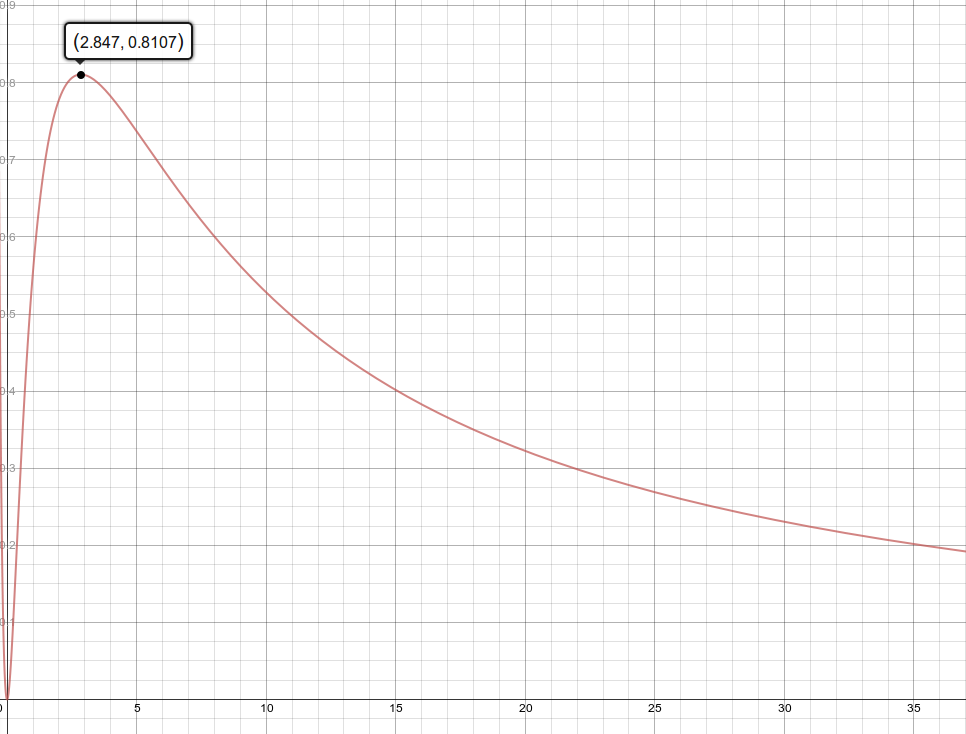
\includegraphics[scale = 0.3]{../tables/model.png}
\end{center}
  


%Now, for all $q \in \{0,\infy \}$, we have $\Delta k_{out-of-copy}>\Delta k_{in-copy}$










































\end{document}



\newpage


%% Table 1 : SUMMARY STATS

%\begin{landscape}
\begin{center}
\begin{table}[!htbp]
\section{Tables and Figures}
%\vspace{5mm}
\caption{Summary Statistics}
\vspace{2.5mm}
\caption*{(1) Sample A: Unit of Observation -- Publication-Year (N=360)}
\vspace{2.5mm}
{
\def\sym#1{\ifmmode^{#1}\else\(^{#1}\)\fi}
\begin{tabular*}{\hsize}{@{\hskip\tabcolsep\extracolsep\fill}l*{1}{rrrrrr}}
\toprule
                              &\multicolumn{5}{c}{}                                            \\
                              &        Mean&          SD&      Median&         Min&         Max\\
\midrule
\emph{Publication-Year}       &     1964.50&       11.56&     1964.50&        1945&        1984\\
\emph{Wikipedia-Year}         &     2008.00&        2.59&     2008.00&        2004&        2012\\
\emph{1(Out-of-Copy)}         &        0.47&        0.50&        0.00&           0&           1\\
\emph{1(Wikipedia-Year$>$2008)}&        0.44&        0.50&        0.00&           0&           1\\
\emph{Total Citations}        &        4.19&        7.84&        0.00&           0&          52\\
\emph{Image Citations}        &        1.20&        4.03&        0.00&           0&          30\\
\emph{Text Citations}         &        2.99&        4.81&        0.00&           0&          22\\
\bottomrule
\end{tabular*}
}

\vspace{2.5mm}
\caption*{(2) Sample B: Unit of Observation -- Player-Page (N=4869)}
\vspace{2.5mm}
{
\def\sym#1{\ifmmode^{#1}\else\(^{#1}\)\fi}
\begin{tabular*}{\hsize}{@{\hskip\tabcolsep\extracolsep\fill}l*{1}{rrrrrr}}
\toprule
                              &\multicolumn{5}{c}{}                                            \\
                              &        Mean&          SD&      Median&         Min&         Max\\
\midrule
\emph{Player Debut-Year}      &     1966.12&       10.19&     1966.00&        1944&        1984\\
\emph{Wikipedia-Year}         &     2008.00&        2.58&     2008.00&        2004&        2012\\
\emph{1(Out-of-Copy)}         &        0.38&        0.49&        0.00&           0&           1\\
\emph{1(Wikipedia-Year$>$2008)}&        0.44&        0.50&        0.00&           0&           1\\
\emph{Total Citations}        &        0.17&        0.86&        0.00&           0&          10\\
\emph{Total Images}           &        0.66&        1.30&        0.00&           0&          18\\
\emph{Total Text}             &        1.18&        1.41&        0.78&           0&          16\\
\emph{Average Traffic}        &      101.49&      224.94&       34.73&           0&        3395\\
\emph{Quality Percentile}     &        2.62&        1.29&        3.00&           1&           4\\
\bottomrule
\end{tabular*}
}

%%{
\def\sym#1{\ifmmode^{#1}\else\(^{#1}\)\fi}
\begin{tabular}{l*{1}{cccc}}
\toprule
                    &\multicolumn{4}{c}{}                               \\
                    &\textbf{(1)out-of-copy $\bar{y}$}&\textbf{(2)in-copy $\bar{y}$}&\textbf{(3)diff}&\textbf{(4)p-val}\\
\midrule
\emph{Number of Citations to Baseball Digest}&       0.597&       0.334&       0.263&        0.03\\
\emph{Number of Images}&       1.888&       1.036&       0.853&        0.00\\
\emph{Number of Words of Text}&      2199.9&      1722.8&       477.1&        0.00\\
\emph{Average Monthly Traffic}&       190.3&       93.35&       96.94&        0.02\\
\bottomrule
\end{tabular}
}

\vspace{5mm}
\label{tab:summary}

\begin{adjustwidth}{-2cm}{-2cm}
\begin{quote}
\emph{Note:} This table presents summary statistics for the two main data samples used in this study. Both samples track citations to Baseball Digest on Wikipedia between 2004 and 2012. In Sample A presented above, the unit of observation is a Publication-Year of Baseball Digest, i.e. all years between 1944 to 1984. For each of the 40 Publication-Years, I track total citations in every Wikipedia-Year between 2004 and 2012, for a sample size of 360 observations (40 issue-years times 9 calendar years). For Sample B, the unit of observation is an individual Wikipedia player-page for 541 notable baseball players. On each player-page, citations to Baseball Digest are tracked (irrespective of the year of publication) between 2004 and 2012, for a total of 4869 observations (541 pages times 9 calendar years). \emph{1(Out-Of-Copy)} is defined as all publication-years (Sample A) or debut-years (Sample B) before 1964. Traffic data is only available for years 2007 to 2013 and data is missing for other observations. See text for detailed data and variable descriptions.
\end{quote}
\end{adjustwidth}

\end{table}
\end{center}
%\end{landscape}

%%% t-test table
%% Table 2 : T-Test Table
%%\begin{landscape}
\begin{center}
\begin{table}[!htbp]
\vspace{15mm}
\caption{Cross-Sectional Comparison of Reuse Outcomes}
\vspace{5mm}

\caption*{\small{\textbf{(1) Sample A : Baseball Digest Publication-Years}}}
\begin{center}
{
\def\sym#1{\ifmmode^{#1}\else\(^{#1}\)\fi}
\begin{tabular}{l*{1}{cccc}}
\toprule
                    &\multicolumn{4}{c}{}                               \\
                    &\textbf{(1)out-of-copy $\bar{y}$}&\textbf{(2)in-copy $\bar{y}$}&\textbf{(3)diff}&\textbf{(4)p-val}\\
\midrule
\emph{Total Citations}&       21.05&       10.33&       10.72&        0.00\\
\emph{Image Citations}&          10&      0.0952&       9.905&        0.00\\
\emph{Text Citations}&       11.05&       10.24&       0.815&        0.60\\
\bottomrule
\end{tabular}
}

\end{center}
\vspace{10mm}

\caption*{\small{\textbf{(2) Sample B : Wikipedia Player-Pages}}}
\begin{center}
{
\def\sym#1{\ifmmode^{#1}\else\(^{#1}\)\fi}
\begin{tabular}{l*{1}{cccc}}
\toprule
                    &\multicolumn{4}{c}{}                               \\
                    &\textbf{(1)out-of-copy $\bar{y}$}&\textbf{(2)in-copy $\bar{y}$}&\textbf{(3)diff}&\textbf{(4)p-val}\\
\midrule
\emph{Total Citations}&       0.602&       0.334&       0.268&        0.03\\
\emph{Total Images} &       1.786&       0.916&       0.870&        0.00\\
\emph{Total Text}   &       2.128&       1.645&       0.483&        0.00\\
\emph{Average Traffic}&       158.9&       111.5&       47.43&        0.03\\
\bottomrule
\end{tabular}
}

\end{center}
\label{tab:ttest}

\begin{quote}
\vspace{5mm}
\emph{Note:} This table compares outcomes for out-of-copyright and in-copyright groups using cross-sectional data from Wikipedia data from 2012. $N=40$ for Panel (1) and $N=541$ for Panel (2). In Panel (1), column (1) includes publication-years 1944-1963, while column (2) includes publication-years 1964-1984. In Panel (2), column (1) includes all out-of-copy player-pages (debut before 1964) and column (2) includes all in-copy player-pages (debut after 1964). The $p$-value reported in Column (4) is from a $t$-test for a difference in mean outcomes across Column (1) and (2). See text for more detailed data and variable descriptions. 
\end{quote}

\end{table}
\end{center}
%%\end{landscape}

%%%%%%%%%
%% Table 3 DD Table
%%%%%%%%%

\begin{center}
\begin{table}[!htbp]
%\caption{Impact of Copyright on Baseball Digest Reuse }
\caption{Impact of 1964 Copyright Experiment on Total Citations}
%\caption{Difference-in-Difference Regressions Estimating Impact of Google Books Digitization Event on Baseball Wikipedia Pages}
\vspace{5mm}
{
\def\sym#1{\ifmmode^{#1}\else\(^{#1}\)\fi}
\begin{tabular*}{\hsize}{@{\hskip\tabcolsep\extracolsep\fill}l*{6}{c}}
\toprule
            &\multicolumn{3}{c}{Sample A}                                     &\multicolumn{3}{c}{Sample B}                                     \\\cmidrule(lr){2-4}\cmidrule(lr){5-7}
            &\multicolumn{1}{c}{Cites}&\multicolumn{1}{c}{Cites}&\multicolumn{1}{c}{Log-Cites}&\multicolumn{1}{c}{Cites}&\multicolumn{1}{c}{Cites}&\multicolumn{1}{c}{Log-Cites}\\
\midrule
\emph{out-of-copy X post}&       5.667         &       5.609         &       0.316         &       0.202         &       0.188         &      0.0690         \\
            &     (1.830)\sym{***}&     (1.809)\sym{***}&     (0.153)\sym{**} &    (0.0588)\sym{***}&     (0.107)\sym{*}  &    (0.0360)\sym{*}  \\
\midrule
Unit of Obs. FE&          No         &         Yes         &         Yes         &          No         &         Yes         &         Yes         \\
Year FE     &         Yes         &         Yes         &         Yes         &         Yes         &         Yes         &         Yes         \\
Page-Age FE &         ---         &         ---         &         ---         &         Yes         &         Yes         &         Yes         \\
adj. $R^2$  &       0.637         &       0.703         &       0.908         &      0.0592         &      0.0851         &       0.116         \\
N           &         360         &         360         &         360         &        4869         &        4869         &        4869         \\
\bottomrule
\end{tabular*}
}

\begin{quote}
\vspace{5mm}

\emph{+:p$<$0.15; *:p$<$0.10; **:p$<$0.05; ***:p$<$0.01 
\newline
Clustered standard errors shown in parentheses.}

\vspace{5mm}

\emph{Note:} This regression estimates the impact of the 1964 copyright exception on affecting citations to Baseball Digest before and after digitization in a differences-in-differences framework using OLS. The estimates presented use both Sample A (columns 1-3) and Sample B (columns 4-6). \emph{post} refers to all Wikipedia-years after 2008, and \emph{out-of-copy} refers either to $publication-year < 1964$ (Sample A) or $debut-year < 1964$ (Sample B). See text for specification, detailed data and variable descriptions.

\end{quote}
\label{tab:maindd}
\end{table}
\end{center}

%% TABLE 4 : Traffic
%%%%%%%% TRAFFIC TABLE

%%% IVREG
\begin{center}
\begin{table}[!htbp]
\caption{Impact of 1964 Copyright Experiment on Wikipedia Traffic (Sample B)}

\vspace{5mm}
{
\def\sym#1{\ifmmode^{#1}\else\(^{#1}\)\fi}
\begin{tabular*}{\hsize}{@{\hskip\tabcolsep\extracolsep\fill}l*{3}{c}}
\toprule
            &\multicolumn{1}{c}{(1)}&\multicolumn{1}{c}{(2)}&\multicolumn{1}{c}{(3)}\\
            &\multicolumn{1}{c}{Traffic}&\multicolumn{1}{c}{Traffic}&\multicolumn{1}{c}{Traffic}\\
\midrule
\emph{out-of-copy X post}&       43.22         &       20.42         &       16.54         \\
            &     (12.09)\sym{***}&     (9.883)\sym{**} &     (10.13)\sym{+}  \\
\midrule
Player-Page FE&          No         &         Yes         &         Yes         \\
Time FE     &     Year FE         &     Year FE         &Quality X Year FE         \\
adj. $R^2$  &      0.0137         &      0.0810         &      0.0899         \\
N           &        3246         &        3246         &        3246         \\
\bottomrule
\end{tabular*}
}

\begin{quote}
\vspace{5mm}
\emph{+:p$<$0.15; *:p$<$0.10; **:p$<$0.05; ***:p$<$0.01 
\newline
Standard errors clustered at player-level shown in parentheses.}
\vspace{5mm}

\emph{Note:} This regression estimates the impact of the 1964 copyright exception on traffic to Wikipedia player-pages before and after digitization in a differences-in-differences framework using OLS. The estimates presented use data from Sample B. \emph{post} refers to all Wikipedia-years after 2008, and \emph{out-of-copy} refers to $debut-year < 1964$. See text for specification, detailed data and variable descriptions. In Column (3) $Quality\ X\ Year\ FE$ controls for separate time-trends by each of the four quartiles of player quality.

\end{quote}
\label{tab:traf}
\end{table}
\end{center}


%% TABLE 5 : DD Images vs. Text
%%%%%%%%%%%%%%%%%%%

\begin{center}
\begin{table}[!htbp]
%\caption{Impact of Copyright on Baseball Digest Reuse }
\caption{Differential Impact of 1964 Copyright Experiment on \\ Image vs. Text Citations (Sample A)}
%\caption{Difference-in-Difference Regressions Estimating Impact of Google Books Digitization Event on Baseball Wikipedia Pages}
\vspace{5mm}
%{
\def\sym#1{\ifmmode^{#1}\else\(^{#1}\)\fi}
\begin{tabular*}{\hsize}{@{\hskip\tabcolsep\extracolsep\fill}l*{3}{c}}
\toprule
                                                  &\multicolumn{1}{c}{OLS}&\multicolumn{1}{c}{OLS}&\multicolumn{1}{c}{Log-OLS}\\
\midrule \vspace{5mm} \makebox[13em][l]{\underline{\textbf{Panel A : Images}}\vspace{5mm} ($\bar{y}$=1.20)}\\
\emph{out-of-copy X post}                         &       5.471         &       5.471         &       1.178         \\
                                                  &     (1.093)\sym{***}&     (1.093)\sym{***}&     (0.152)\sym{***}\\

\end{tabular*} }
{
\def\sym#1{\ifmmode^{#1}\else\(^{#1}\)\fi}
\begin{tabular*}{\hsize}{@{\hskip\tabcolsep\extracolsep\fill}l*{3}{c}}
\midrule \vspace{5mm} \makebox[13em][l]{\underline{\textbf{Panel B : Text}}\vspace{5mm} ($\bar{y}$=2.99)}\\
\emph{out-of-copy X post}                         &       0.354         &       0.328         &     0.00783         \\
                                                  &     (1.023)         &     (1.009)         &     (0.141)         \\
\midrule
Issue-Year FE                                     &          No         &         Yes         &         Yes         \\
Time FE                                           &        Year         &        Year         &        Year         \\
N                                                 &         360         &         360         &         360         \\
Adj R-square                                      &       0.737         &       0.812         &       0.918         \\
\bottomrule
\end{tabular*}
}

%{
\def\sym#1{\ifmmode^{#1}\else\(^{#1}\)\fi}
\begin{tabular*}{\hsize}{@{\hskip\tabcolsep\extracolsep\fill}l*{3}{c}}
\toprule
                                                  &\multicolumn{1}{c}{OLS}&\multicolumn{1}{c}{OLS}&\multicolumn{1}{c}{Log-OLS}\\
\midrule \makebox[13em][l]{\underline{\textbf{Sample A : Images}} \vspace{5mm} ($\bar{y}$=1.20)}\\
\emph{out-of-copy X post}                         &       5.471         &       5.471         &       1.178         \\
                                                  &     (1.093)\sym{***}&     (1.093)\sym{***}&     (0.152)\sym{***}\\

\end{tabular*} }
{
\def\sym#1{\ifmmode^{#1}\else\(^{#1}\)\fi}
\begin{tabular*}{\hsize}{@{\hskip\tabcolsep\extracolsep\fill}l*{3}{c}}
\midrule \vspace{5mm} \makebox[13em][l]{\underline{\textbf{Sample A : Text}}\vspace{5mm} ($\bar{y}$=2.99)}\\
\emph{out-of-copy X post}                         &       0.354         &       0.328         &     0.00783         \\
                                                  &     (1.023)         &     (1.009)         &     (0.141)         \\

\end{tabular*} }
{
\def\sym#1{\ifmmode^{#1}\else\(^{#1}\)\fi}
\begin{tabular*}{\hsize}{@{\hskip\tabcolsep\extracolsep\fill}l*{3}{c}}
\midrule \vspace{5mm} \makebox[13em][l]{\underline{\textbf{Sample B : Images}}\vspace{5mm} ($\bar{y}$=0.50)}\\
\emph{out-of-copy X post}                         &       0.549         &       0.381         &       0.113         \\
                                                  &     (0.147)\sym{***}&     (0.119)\sym{***}&    (0.0389)\sym{***}\\

\end{tabular*} }
{
\def\sym#1{\ifmmode^{#1}\else\(^{#1}\)\fi}
\begin{tabular*}{\hsize}{@{\hskip\tabcolsep\extracolsep\fill}l*{3}{c}}
\midrule \vspace{5mm} \makebox[13em][l]{\underline{\textbf{Sample B : Text}}\vspace{5mm} ($\bar{y}$=0.89)}\\
\emph{out-of-copy X post}                         &       0.441         &       0.311         &      0.0593         \\
                                                  &     (0.156)\sym{***}&     (0.114)\sym{***}&    (0.0247)\sym{**} \\
\midrule
Unit of Obs. FE                                   &          No         &         Yes         &         Yes         \\
Time FE                                           &        Year         &        Year         &        Year         \\
\bottomrule
\end{tabular*}
}

{
\def\sym#1{\ifmmode^{#1}\else\(^{#1}\)\fi}
\begin{tabular*}{\hsize}{@{\hskip\tabcolsep\extracolsep\fill}l*{6}{c}}
\toprule
            &\multicolumn{3}{c}{Images}                                       &\multicolumn{3}{c}{Text}                                         \\\cmidrule(lr){2-4}\cmidrule(lr){5-7}
            &\multicolumn{1}{c}{OLS}&\multicolumn{1}{c}{OLS}&\multicolumn{1}{c}{Log-OLS}&\multicolumn{1}{c}{OLS}&\multicolumn{1}{c}{OLS}&\multicolumn{1}{c}{Log-OLS}\\
\midrule
\emph{out-of-copy X post}&       5.471         &       5.471         &       1.178         &       0.354         &       0.328         &     0.00783         \\
            &     (1.093)\sym{***}&     (1.093)\sym{***}&     (0.152)\sym{***}&     (1.023)         &     (1.009)         &     (0.141)         \\
\midrule
Publication-Year FE&          No         &         Yes         &         Yes         &          No         &         Yes         &         Yes         \\
Year FE     &         Yes         &         Yes         &         Yes         &         Yes         &         Yes         &         Yes         \\
adj. $R^2$  &       0.415         &       0.417         &       0.574         &       0.737         &       0.812         &       0.918         \\
N           &         360         &         360         &         360         &         360         &         360         &         360         \\
\bottomrule
\end{tabular*}
}

%\vspace{5mm}
%\caption*{Panel B}
%{
\def\sym#1{\ifmmode^{#1}\else\(^{#1}\)\fi}
\begin{tabular*}{\hsize}{@{\hskip\tabcolsep\extracolsep\fill}l*{3}{c}}
\toprule
                                                  &\multicolumn{1}{c}{OLS}&\multicolumn{1}{c}{OLS}&\multicolumn{1}{c}{Log-OLS}\\
\midrule \vspace{5mm} \makebox[13em][l]{\underline{\textbf{Panel A : Images}}\vspace{5mm} ($\bar{y}$=0.66)}\\
\emph{out-of-copy X post}                         &       0.280         &       0.226         &      0.0646         \\
                                                  &     (0.106)\sym{***}&     (0.105)\sym{**} &    (0.0352)\sym{*}  \\

\end{tabular*} }
{
\def\sym#1{\ifmmode^{#1}\else\(^{#1}\)\fi}
\begin{tabular*}{\hsize}{@{\hskip\tabcolsep\extracolsep\fill}l*{3}{c}}
\midrule \vspace{5mm} \makebox[13em][l]{\underline{\textbf{Panel B : Text}}\vspace{5mm} ($\bar{y}$=1179.96)}\\
\emph{out-of-copy X post}                         &       234.9         &       205.9         &     -0.0466         \\
                                                  &     (96.06)\sym{**} &     (98.08)\sym{**} &    (0.0955)         \\
\midrule
Player-Page FE                                    &         Yes         &         Yes         &         Yes         \\
Time FE                                           &        Year         &Quality X Year         &        Year         \\
N                                                 &        4869         &        4869         &        4869         \\
Adj R-square                                      &       0.397         &       0.404         &       0.613         \\
\bottomrule
\end{tabular*}
}



\begin{quote}
\vspace{5mm}

\emph{+:p$<$0.15; *:p$<$0.10; **:p$<$0.05; ***:p$<$0.01 
\newline
Clustered standard errors shown in parentheses.}

\vspace{5mm}

\emph{Note:} This regression estimates the impact of the 1964 copyright exception on affecting the reuse of images and text from Baseball Digest before and after digitization in a differences-in-differences framework. The estimates presented use data from Sample A. \emph{post} refers to all Wikipedia-years after 2008, and \emph{out-of-copy} refers to $publication-year < 1964$. See text for specification, detailed data and variable descriptions.
\end{quote}
\label{tab:imgdd}
\end{table}
\end{center}









%%%%%%%%%%%%%%%%%%%%%%%%%%%%%%%%%%%%%%%%%%%%%%
%%%%%%%%%%%%%%%%%% FIGURE  %%%%%%%%%%%%%%%%%%%
%%%%%%%%%%%%%%%%%%%%%%%%%%%%%%%%%%%%%%%%%%%%%%
%\newpage

%% Fig 1 : Schematic
\begin{figure}[!htbp]
\begin{center}
\caption{An Illustration of How Copyright Might Affect the Reuse of Information}
\label{fig:cover}
\vspace{5mm}
\caption*{(1) Felipe Alou's image in December 1963 (out-of-copyright) issue of Baseball Digest, reused on Wikipedia)}
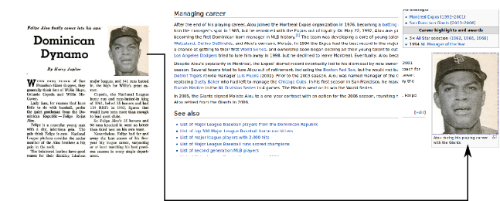
\includegraphics[scale=1]{../tables/cover_bottom.png}
\vspace{2mm}
\caption*{(2) Johnny Callison's image in January 1964 (in-copyright) issue of Baseball Digest, not reused on Wikipedia}
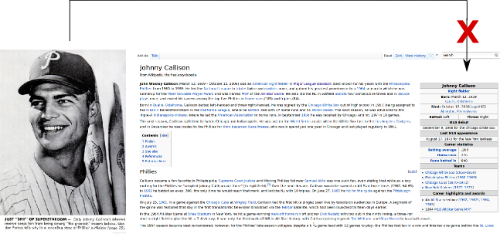
\includegraphics[scale=1]{../tables/cover_top.png}

\end{center}
\begin{quote}
\vspace{5mm}
\end{quote}
\end{figure}

%%% Fig 2: mean charts, digitization
\begin{figure}[!htbp]
\begin{center}
\caption{Citations to Baseball Digest on Wikipedia (Sample A)}
\label{fig:overview}
\caption*{(1) Citations to Baseball Digest before and after Digitization}
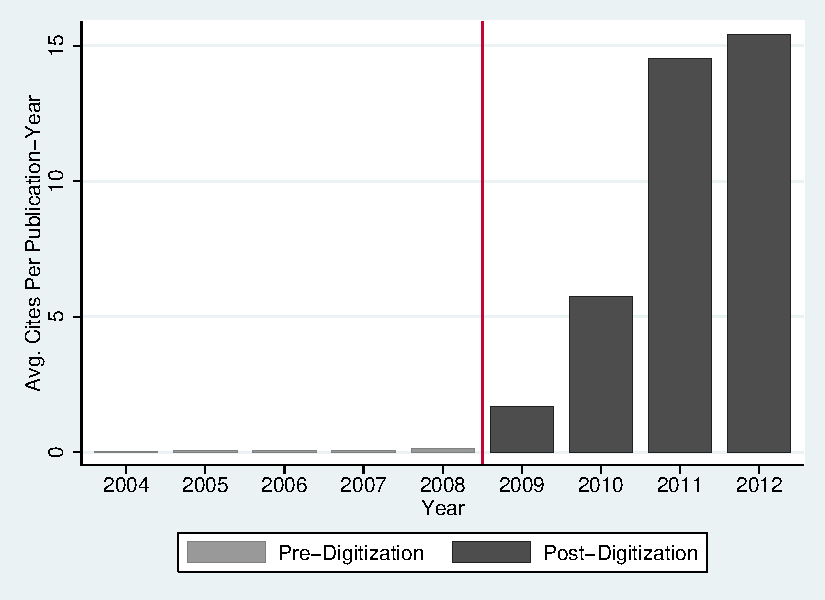
\includegraphics[scale=0.75]{../tables/mean_digit.pdf}
\vspace{5mm}
\caption*{(2) Citations to Baseball Digest for issues published before and after 1964}
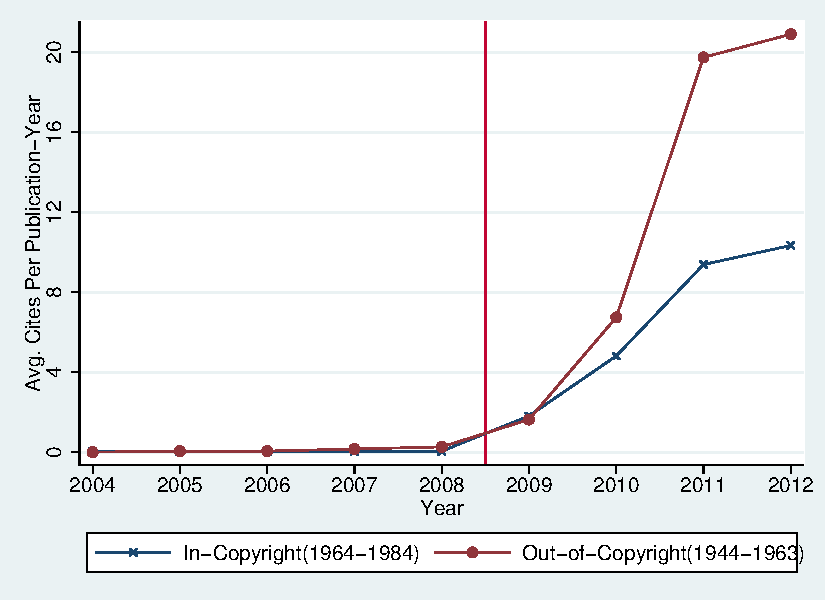
\includegraphics[scale=0.75]{../tables/mean_connected_cites.pdf}
%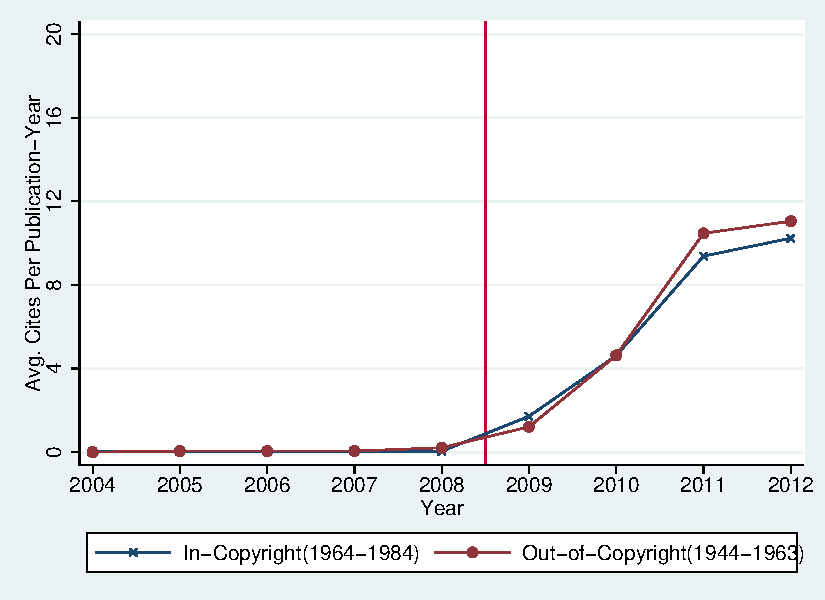
\includegraphics[scale=0.25]{../tables/mean_connected_text.pdf}
%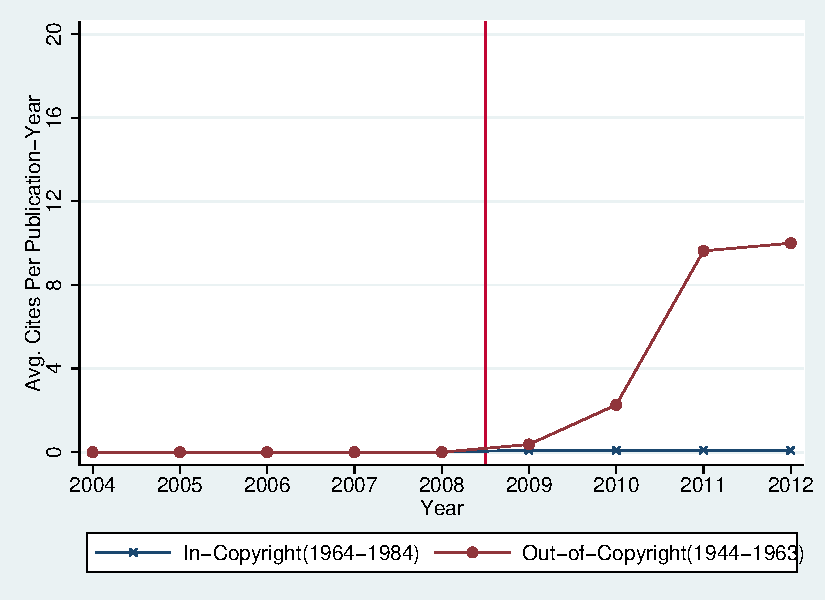
\includegraphics[scale=0.25]{../tables/mean_connected_img.pdf}
\end{center}

\begin{quote}
\emph{Note:} This plot presents some simple descriptive data on citations to Baseball Digest issues. Panel (1) presents average citations per publication-year of Baseball Digest on Wikipedia before and after the Google Books digitization event in 2008. Panel (2) presents similar information, but data are presented separately for all publication-years before 1964 (out-of-copyright) and those in or after 1964 (in-copyright). See text for more detailed data and variable descriptions. 
\end{quote}
\end{figure}

%% Fig 3. DD picture
%\begin{landscape}

\begin{figure}[!htbp]
\begin{center}
\caption{Time-Varying Estimates of the Impact of Copyright\\ on Citations to Baseball Digest}
\label{fig:ddpic}
\caption*{(1) Sample A : Total Citations}
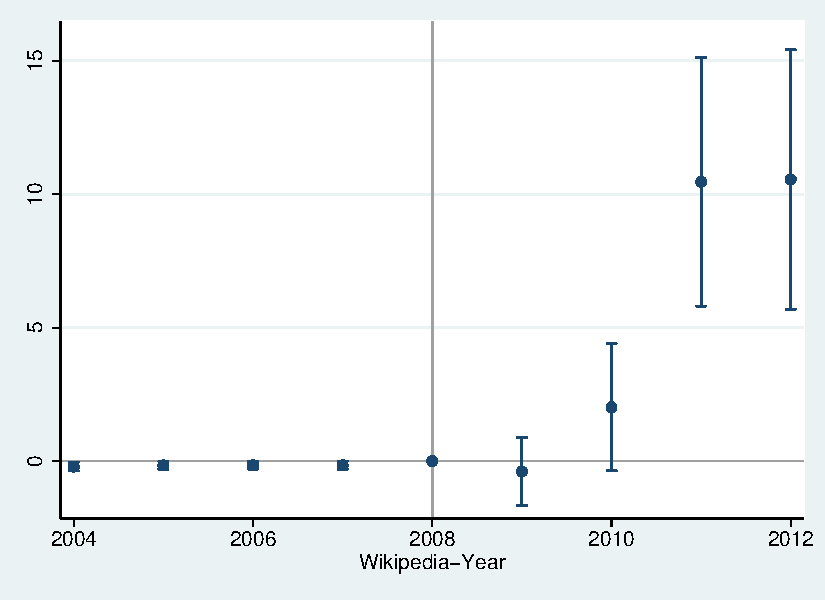
\includegraphics[scale=0.7]{../tables/cite_timeline_cites.pdf}
\vspace{2mm}
\caption*{(2) Sample B : Total Citations}
%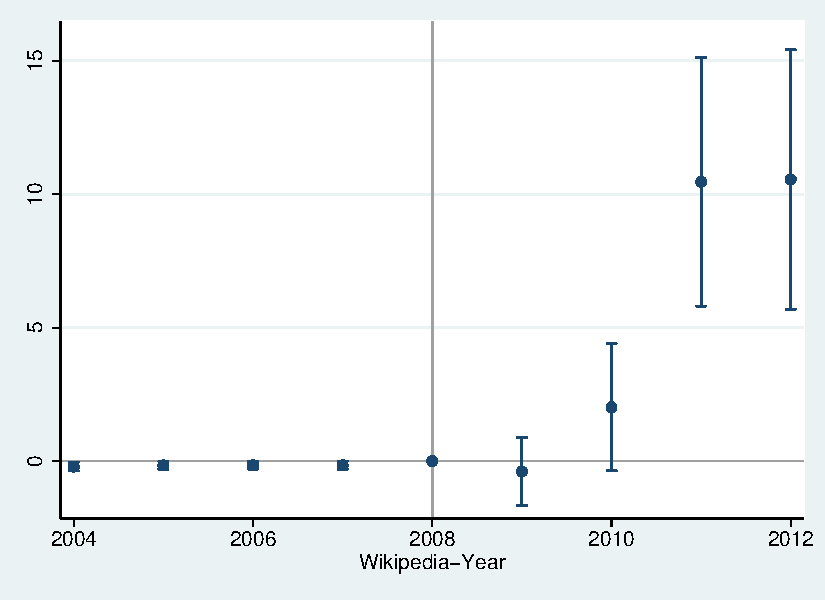
\includegraphics[scale=0.6]{../tables/cite_timeline_cites.pdf}
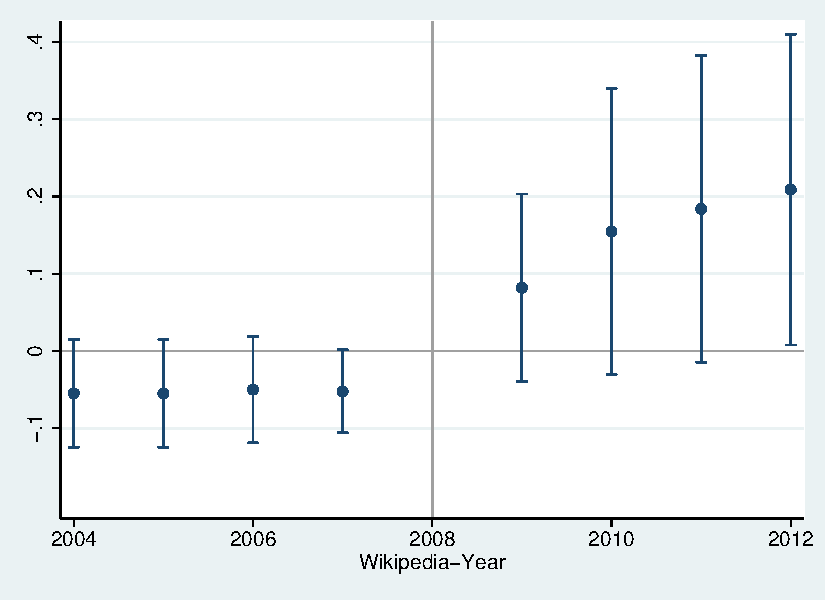
\includegraphics[scale=0.7]{../tables/timeline_bd_1.pdf}

%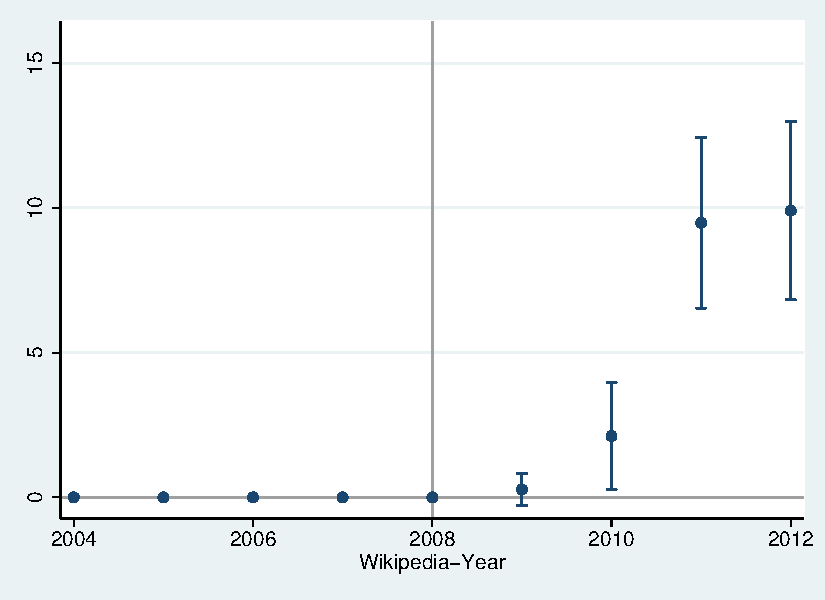
\includegraphics[scale=0.6]{../tables/cite_timeline_img.pdf}
%\vspace{5mm}
%\caption*{Panel B : Basketball Players}
%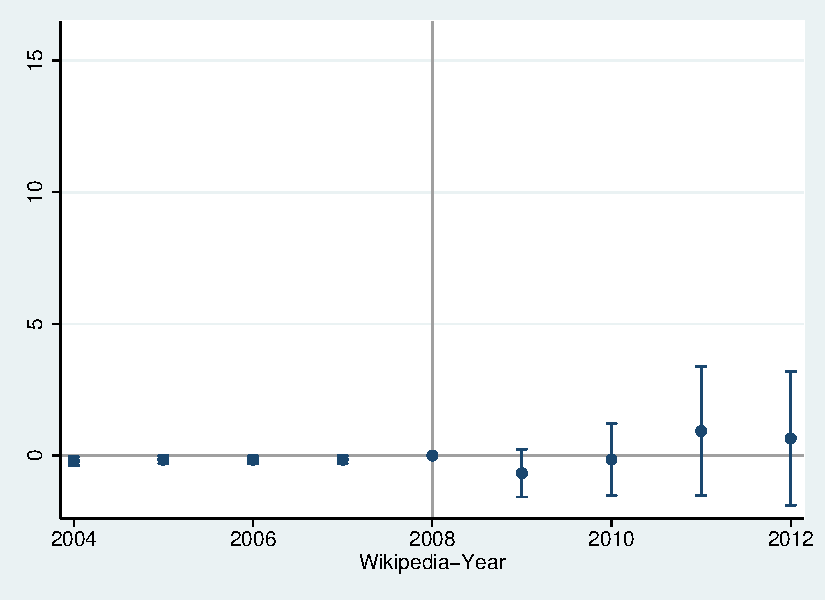
\includegraphics[scale=0.6]{../tables/cite_timeline_text.pdf}
\end{center}

\begin{quote}
%\begin{adjustwidth}{-2cm}{-2cm}
\emph{Note:} This figure plots coefficients (and 95 percent confidence intervals) from the event study specifications described in Section \ref{sec:timevary}. On the $x$ axis is the Wikipedia-year and the reference year is 2008, the year of the digitization event. This specification is based on Sample A for Panel (1) and Sample B for Panel (2), the coefficients are estimates from ordinary-least-squares (OLS) models, and standard errors are clustered. The dependent variable in both panels is the total number of citations in a calendar year. See text for more detailed data and variable descriptions. 
%\end{adjustwidth}

\end{quote}
\end{figure}
%\end{landscape}


%Fig 4. Killer Pic Sample A
%\begin{landscape}

\begin{figure}[!htbp]
\begin{center}
\caption{Citations to Baseball Digest Published Before and After the 1964 Copyright Cutoff (Sample A)}
\label{fig:killer_cite}
%\caption*{Panel A : Citation Gains at the Issue-Year Level between 2012 and 2008}
\vspace{1cm}

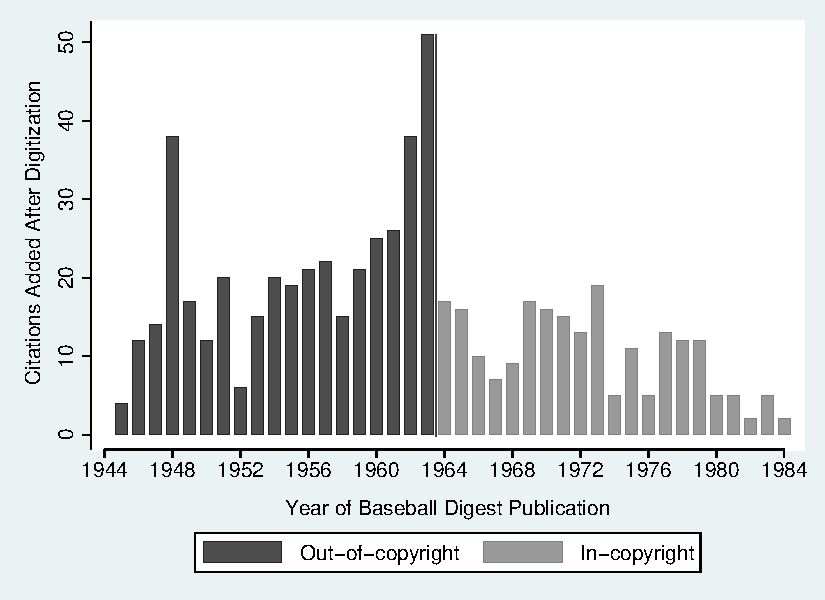
\includegraphics[scale=1]{../tables/cite_killer_cite.pdf}
%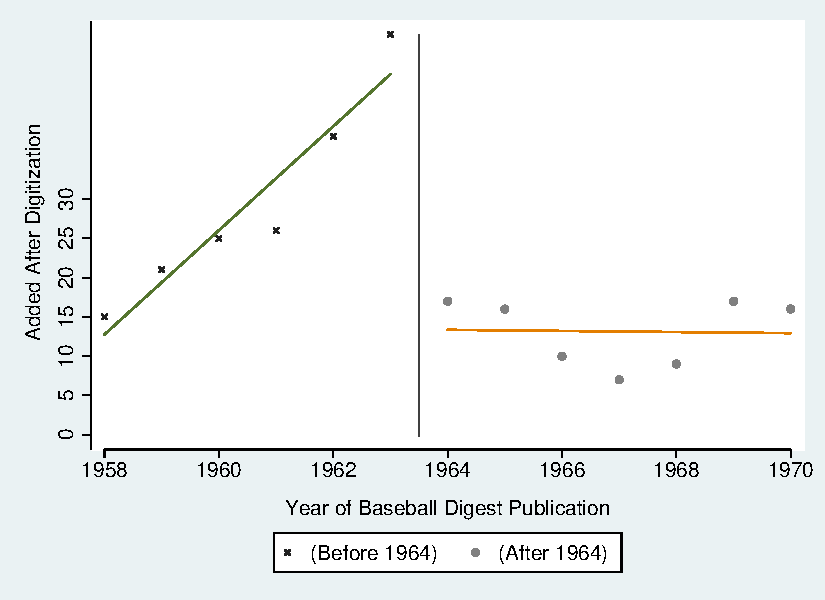
\includegraphics[scale=1]{../tables/cite_scatter_cite.pdf}


%\vspace{2mm}
%\caption*{Panel B : Comparing Citation Gains For Image Reuse and In-Text Citations}
%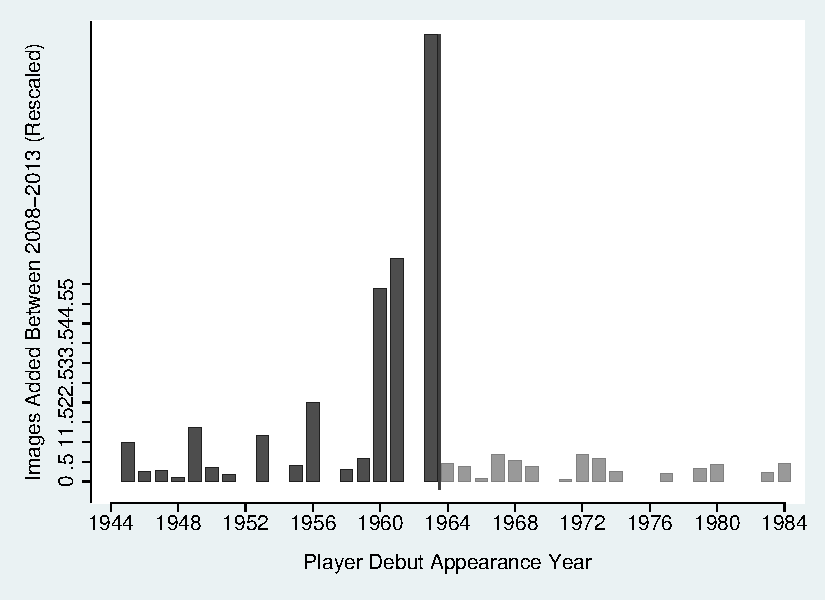
\includegraphics[scale=0.75]{../tables/killerpic2_1_bd.pdf}

%\includegraphics[scale=0.65]{../tables/cite_killer_img.pdf}
%\vspace{5mm}
%\caption*{Panel B : Basketball Players}
%\includegraphics[scale=0.65]{../tables/cite_killer_text.pdf}
\end{center}
\vspace{1cm}
\begin{quote}
%\begin{adjustwidth}{-2cm}{-2cm}
\emph{Note:} This figure plots the growth in citations to Baseball Digest publication-years in 2012 as compared to 2008. Out-of-copyright publication-years (1944-1963) are shown in dark grey, while in-copyright publication-years (1964-1984) are shown in light grey. See text for more detailed data and variable descriptions. 
%\end{adjustwidth}

\end{quote}
\end{figure}
%\end{landscape}

\newpage


%\newpage
%%\begin{landscape}
%%%%% Fig 5. Killer Pic for Images and Text

\newpage
%\begin{landscape}

\begin{figure}[!htbp]
\begin{center}
\caption{Impact of Copyright on Image and Text Citations (Sample A)}
\label{fig:killer_img}
\caption*{(1) Image Citations}

\includegraphics[scale=0.7]{../tables/cite_killer_img.pdf}

\vspace{0.2cm}
\caption*{(2) Text Citations}
\includegraphics[scale=0.75]{../tables/cite_killer_text.pdf}

%\includegraphics[scale=0.25]{../tables/mean_connected_text.pdf}
%\includegraphics[scale=0.25]{../tables/mean_connected_img.pdf}
\vspace{5mm}

%\caption*{Panel B : Time Varying Estimates of the Impact of Copyright on Wikipedia Pages}
%\includegraphics[scale=0.65]{../tables/killerpic2_1_img.pdf}
%\includegraphics[scale=0.65]{../tables/killerpic2_1_text.pdf}
%\includegraphics[scale=0.75]{../tables/timeline_img_1.pdf}
%\includegraphics[scale=0.25]{../tables/mean_connected_text.pdf}
%\includegraphics[scale=0.25]{../tables/mean_connected_img.pdf}
\end{center}

\begin{quote}
%\begin{adjustwidth}{-2cm}{-2cm}
%\emph{Note:} This chart documents the impact of the 1964 copyright cutoff for Baseball Digest on the reuse of images and text

\emph{Note:} This figure plots the growth in citations to Baseball Digest publication-years in 2012 as compared to 2008. Panel (1) plots the growth in Image citations, while Panel (2) plots the growth in Text citations. Out-of-copyright publication-years (1944-1963) are shown in dark grey, while in-copyright publication-years (1964-1984) are shown in light grey. See text for more detailed data and variable descriptions. 


%number of images added to baseball Wikipedia pages. Panel A documents the variation in the number of images added between 2008 and 2013 for out-of-copyright (debut before 1964) players and in-copyright (debut after 1964) players. The raw mean is adjusted to account for each player's differing exposure to the copyright rule. Panel B plots coefficients (and 95 percent confidence intervals) from the event study specifications described in Section \ref{sec:timevary}. On the $x$ axis is the calendar year and the reference year is 2008, the year of the digitization event. This specification is based on page-year level observations, the coefficients are estimates from ordinary-least-squares (OLS) models, and standard errors are clustered at the page level. See text for more detailed data and variable descriptions. 
%\end{adjustwidth}
\end{quote}
\end{figure}

%\end{landscape}

%%%%%%%%%%%
%%%%% Fig 6. DD Pic 2 for Images and Text
%%%%%%%%%%%

\begin{figure}[!htbp]
\begin{center}
\caption{Time-Varying Estimates for Image and Text Citations (Sample A)}
\label{fig:ddpic_img}
\caption*{\small{(1) Image Citations}}
%\includegraphics[scale=0.75]{../tables/cite_timeline_cites.pdf}
\includegraphics[scale=0.75]{../tables/cite_timeline_img.pdf}

\caption*{\small{(2) Text Citations}}
\includegraphics[scale=0.75]{../tables/cite_timeline_text.pdf}
\vspace{2mm}

%\caption*{Sample B : }
%\includegraphics[scale=0.6]{../tables/timeline_img_1.pdf}
%\includegraphics[scale=0.6]{../tables/timeline_text_1.pdf}

%\includegraphics[scale=0.6]{../tables/cite_timeline_cites.pdf}

%\includegraphics[scale=0.6]{../tables/cite_timeline_img.pdf}
%\vspace{5mm}
%\caption*{Panel B : Basketball Players}
%\includegraphics[scale=0.6]{../tables/cite_timeline_text.pdf}
\end{center}

\begin{quote}
\emph{Note:} This figure plots coefficients (and 95 percent confidence intervals) from the event study specifications described in Section \ref{sec:timevary} separately for image (Panel 1) and text citations (Panel 2). On the $x$ axis is the Wikipedia-year and the reference year is 2008, the year of the digitization event. This specification is based on Sample A for Panel (1) and (2). The coefficients are estimated from ordinary-least-squares (OLS) models, and standard errors are clustered. The dependent variable in both panels is the total number of citations in a calendar year. See text for more detailed data and variable descriptions. 

\end{quote}
\end{figure}



%%%%%%%%%%%
%%% Fig 7: HETERO EFFECTS
%%%%%%%%%%%

\begin{figure}[!htbp]
\begin{center}
\caption{Heterogeneous Impacts of Copyright on Wikipedia Pages by Player Quality (Sample B)}
\label{fig:quality}
\vspace{5mm}
\caption*{\small{(1) Images}}
\includegraphics[scale=0.70]{../tables/quality_img.pdf}\\
\vspace{5mm}
\caption*{\small{(2) Traffic}}
\includegraphics[scale=0.70]{../tables/quality_traf.pdf}

\end{center}
\begin{quote}
%\begin{adjustwidth}{-2cm}{-2cm}
\emph{Note:} This plot documents the differential impact of the Baseball Digest copyright cutoff on baseball player pages of different \emph{quality} as described in Section \ref{sec:diff2}. For this analysis, players are split into 4 different levels of quality based on their percentile rank within the sample of baseball players and the main difference-in-difference estimates are calculated separately for each of the four quality percentiles. Panel (1) plots these estimates for Image Citations, while Panel (2) plots estimates for Traffic. See text for detailed data and variable descriptions.

%%Coefficients ($\beta_3$) are derived from the specification: 

%%$Y_{it} = \alpha + \beta_1 \times post_t \times out-of-copy_i + \beta_2 \times post_t \times quality_i + \beta_3 \times post_t \times out-of-copy_i \times quality_i + \gamma_i+ \delta_t + \epsilon_{it}$ 

%%where $\gamma_{i}$ and $\delta_{t}$ represents player and time fixed effects respectively for player $i$ and year $t$.  All estimates are from ordinary-least-squares (OLS) models. 

%\end{adjustwidth}
\end{quote}
\end{figure}

%%\end{landscape}

%%%%%%%%%%%%%%%% APPENDIX %%%%%%%%%%%%%%%%%%%%%%%%%%%
%blank
%\newpage
%\newpage

\appendix

\setcounter{table}{0}\renewcommand{\thetable}{A.\arabic{table}}
\setcounter{figure}{0}\renewcommand{\thefigure}{A.\arabic{figure}}

%%%%% DD Table %%%%
\begin{center}
\begin{table}[!htbp]
\section{Appendices}

\subsection{Appendix A1 : Robustness Checks}
\label{sec:envelope}

%% BASKETBALL DATA Added

\caption{Estimating the Causal Impact of Digitization}
\vspace{5mm}
{
\def\sym#1{\ifmmode^{#1}\else\(^{#1}\)\fi}
\begin{tabular*}{\hsize}{@{\hskip\tabcolsep\extracolsep\fill}l*{3}{c}}
\toprule
            &\multicolumn{3}{c}{Digitization DD}                              \\\cmidrule(lr){2-4}
            &\multicolumn{1}{c}{Citations}&\multicolumn{1}{c}{Images}&\multicolumn{1}{c}{Text}\\
\midrule
\emph{baseball X post}&       0.340         &       0.459         &       0.391         \\
            &    (0.0494)\sym{***}&    (0.0610)\sym{***}&    (0.0650)\sym{***}\\
\midrule
Player FE   &         Yes         &         Yes         &         Yes         \\
Time FE     &        Year         &        Year         &        Year         \\
adj. $R^2$  &      0.0687         &       0.172         &       0.399         \\
N           &       13260         &       13260         &       13260         \\
Clusters    &        1105         &        1105         &        1105         \\
\bottomrule
\end{tabular*}
}

\begin{quote}
\vspace{5mm}

\emph{+:p$<$0.15; *:p$<$0.10; **:p$<$0.05; ***:p$<$0.01 
\newline
Standard errors clustered at player-level shown in parentheses.}

\vspace{5mm}

\emph{Note:} This table provides estimates that help to determine the causal impact of the Google Books digitization event on reuse. I supplement data in Sample B, with similar data from Wikipedia player-pages for a comparable set of 564 basketball players. The estimates are provided from a difference-in-difference specification where the treatment group is the set of baseball player-pages and the post-period are the years 2009-2012 after the digitization event. All estimates are from ordinary-least-squares (OLS) models. See text for detailed data and variable descriptions.
\end{quote}
\label{tab:basketball}
\end{table}
\end{center}



%%% LEADS - LAGS
\begin{center}
\begin{table}[!htbp]

\caption{Robustness: Exploring pre-trends between in-copyright and out-of-copyright Issues}
%\vspace{5mm}
{\small
{
\def\sym#1{\ifmmode^{#1}\else\(^{#1}\)\fi}
\begin{tabular*}{\hsize}{@{\hskip\tabcolsep\extracolsep\fill}l*{6}{c}}
\toprule
            &\multicolumn{3}{c}{Sample A}                                     &\multicolumn{3}{c}{Sample B}                                     \\\cmidrule(lr){2-4}\cmidrule(lr){5-7}
            &\multicolumn{1}{c}{Citations}&\multicolumn{1}{c}{Images}&\multicolumn{1}{c}{Text}&\multicolumn{1}{c}{Citations}&\multicolumn{1}{c}{Images}&\multicolumn{1}{c}{Text}\\
\midrule
$Digitization_{-3}$&      -0.000         &      -0.000         &      -0.000         &      -0.008         &      -0.194         &      -0.642         \\
            &         (.)         &     (0.000)         &     (0.000)         &     (0.004)\sym{*}  &     (0.024)\sym{***}&     (0.031)\sym{***}\\
\addlinespace
$Digitization_{-2}$&      -0.000         &      -0.000         &      -0.000         &      -0.008         &      -0.075         &      -0.359         \\
            &         (.)         &     (0.000)         &     (0.000)         &     (0.004)\sym{**} &     (0.027)\sym{***}&     (0.022)\sym{***}\\
\addlinespace
$Digitization_{-1}$&      -0.000         &      -0.000         &      -0.000         &      -0.003         &      -0.033         &      -0.106         \\
            &     (0.000)         &     (0.000)         &     (0.000)         &     (0.003)         &     (0.019)\sym{*}  &     (0.009)\sym{***}\\
\addlinespace
$Digitization_{+1}$&       1.762         &       0.095         &       1.667         &       0.046         &       0.060         &       0.088         \\
            &     (0.424)\sym{***}&     (0.066)         &     (0.421)\sym{***}&     (0.015)\sym{***}&     (0.016)\sym{***}&     (0.007)\sym{***}\\
\addlinespace
$Digitization_{+2}$&       4.762         &       0.095         &       4.667         &       0.112         &       0.140         &       0.220         \\
            &     (0.680)\sym{***}&     (0.066)         &     (0.681)\sym{***}&     (0.027)\sym{***}&     (0.020)\sym{***}&     (0.012)\sym{***}\\
\addlinespace
$Digitization_{+3}$&       9.333         &       0.095         &       9.238         &       0.128         &       0.220         &       0.397         \\
            &     (1.064)\sym{***}&     (0.066)         &     (1.060)\sym{***}&     (0.028)\sym{***}&     (0.026)\sym{***}&     (0.017)\sym{***}\\
\addlinespace
$Digitization_{+4}$&      10.286         &       0.095         &      10.190         &       0.132         &       0.259         &       0.472         \\
            &     (1.195)\sym{***}&     (0.066)         &     (1.189)\sym{***}&     (0.028)\sym{***}&     (0.026)\sym{***}&     (0.020)\sym{***}\\
\addlinespace
$Digitization_{-3}$ x out-of-copy&      -0.211         &       0.000         &      -0.211         &      -0.040         &      -0.093         &      -0.180         \\
            &     (0.097)\sym{**} &     (0.000)         &     (0.097)\sym{**} &     (0.027)\sym{+}  &     (0.064)\sym{+}  &     (0.084)\sym{**} \\
\addlinespace
$Digitization_{-2}$ x out-of-copy&      -0.211         &       0.000         &      -0.211         &      -0.037         &      -0.013         &      -0.127         \\
            &     (0.097)\sym{**} &     (0.000)         &     (0.097)\sym{**} &     (0.027)         &     (0.062)         &     (0.067)\sym{*}  \\
\addlinespace
$Digitization_{-1}$ x out-of-copy&      -0.105         &       0.000         &      -0.105         &      -0.035         &       0.033         &      -0.114         \\
            &     (0.073)         &     (0.000)         &     (0.073)         &     (0.021)\sym{*}  &     (0.052)         &     (0.050)\sym{**} \\
\addlinespace
$Digitization_{+1}$ x out-of-copy&      -0.393         &       0.273         &      -0.667         &       0.077         &      -0.038         &       0.050         \\
            &     (0.757)         &     (0.327)         &     (0.544)         &     (0.045)\sym{*}  &     (0.042)         &     (0.024)\sym{**} \\
\addlinespace
$Digitization_{+2}$ x out-of-copy&       1.712         &       2.115         &      -0.404         &       0.160         &      -0.013         &       0.124         \\
            &     (1.443)         &     (1.100)\sym{*}  &     (0.834)         &     (0.068)\sym{**} &     (0.055)         &     (0.039)\sym{***}\\
\addlinespace
$Digitization_{+3}$ x out-of-copy&      10.140         &       9.484         &       0.657         &       0.187         &       0.383         &       0.101         \\
            &     (2.762)\sym{***}&     (1.748)\sym{***}&     (1.453)         &     (0.073)\sym{**} &     (0.083)\sym{***}&     (0.046)\sym{**} \\
\addlinespace
$Digitization_{+4}$ x out-of-copy&      10.346         &       9.905         &       0.441         &       0.206         &       0.454         &       0.117         \\
            &     (2.938)\sym{***}&     (1.826)\sym{***}&     (1.581)         &     (0.074)\sym{***}&     (0.086)\sym{***}&     (0.055)\sym{**} \\
\midrule
Player FE   &         Yes         &         Yes         &         Yes         &         Yes         &         Yes         &         Yes         \\
Time FE     &        Year         &        Year         &        Year         &        Year         &        Year         &        Year         \\
adj. $R^2$  &       0.748         &       0.573         &       0.799         &       0.043         &       0.134         &       0.365         \\
N           &     360.000         &     360.000         &     360.000         &    9945.000         &    9945.000         &    9945.000         \\
\bottomrule
\end{tabular*}
}

}
\begin{quote}
\vspace{5mm}

\emph{+:p$<$0.15; *:p$<$0.10; **:p$<$0.05; ***:p$<$0.01 
\newline
Standard errors clustered at player-level shown in parentheses.}

\vspace{5mm}

%\emph{Note:} This table presents XXX
\end{quote}
\label{tab:leads_lags}
\end{table}
\end{center}

%%% Falsitifction
\begin{center}
\begin{table}[!htbp]

\caption{Falsification Check -- Alternate Treatment Years}
\vspace{5mm}
%{
\def\sym#1{\ifmmode^{#1}\else\(^{#1}\)\fi}
\begin{tabular*}{\hsize}{@{\hskip\tabcolsep\extracolsep\fill}l*{6}{c}}
\toprule
            &\multicolumn{3}{c}{Sample A}                                     &\multicolumn{3}{c}{Sample B}                                     \\\cmidrule(lr){2-4}\cmidrule(lr){5-7}
            &\multicolumn{1}{c}{Citations}&\multicolumn{1}{c}{Images}&\multicolumn{1}{c}{Text}&\multicolumn{1}{c}{Citations}&\multicolumn{1}{c}{Images}&\multicolumn{1}{c}{Text}\\
\midrule
\emph{out-of-copy X post}&    -0.00835         &      0.0911         &     -0.0994         &      0.0631         &      0.0631         &      0.0631         \\
            &     (0.266)         &     (0.108)         &     (0.195)         &    (0.0398)         &    (0.0398)         &    (0.0398)         \\
\midrule
Player FE   &         Yes         &         Yes         &         Yes         &         Yes         &         Yes         &         Yes         \\
Time FE     &        Year         &        Year         &        Year         &        Year         &        Year         &        Year         \\
adj. $R^2$  &       0.320         &      0.0314         &       0.385         &      0.0350         &      0.0350         &      0.0350         \\
N           &         240         &         240         &         240         &        3246         &        3246         &        3246         \\
\bottomrule
\end{tabular*}
}

{
\def\sym#1{\ifmmode^{#1}\else\(^{#1}\)\fi}
\begin{tabular*}{\hsize}{@{\hskip\tabcolsep\extracolsep\fill}l*{6}{c}}
\toprule
            &\multicolumn{3}{c}{Sample A}                                     &\multicolumn{3}{c}{Sample B}                                     \\\cmidrule(lr){2-4}\cmidrule(lr){5-7}
            &\multicolumn{1}{c}{Cites}&\multicolumn{1}{c}{Cites}&\multicolumn{1}{c}{Log-Cites}&\multicolumn{1}{c}{Cites}&\multicolumn{1}{c}{Cites}&\multicolumn{1}{c}{Log-Cites}\\
\midrule
\emph{out-of-copy X post}&     -0.0209         &    -0.00835         &     -0.0105         &      0.0685         &      0.0631         &      0.0207         \\
            &     (0.296)         &     (0.266)         &    (0.0768)         &    (0.0323)\sym{**} &    (0.0398)         &    (0.0145)         \\
\midrule
Unit of Obs. FE&          No         &         Yes         &         Yes         &          No         &         Yes         &         Yes         \\
Year FE     &         Yes         &         Yes         &         Yes         &         Yes         &         Yes         &         Yes         \\
adj. $R^2$  &       0.256         &       0.320         &       0.541         &      0.0265         &      0.0350         &      0.0441         \\
N           &         240         &         240         &         240         &        3246         &        3246         &        3246         \\
\bottomrule
\end{tabular*}
}

\begin{quote}
\vspace{5mm}

\emph{+:p$<$0.15; *:p$<$0.10; **:p$<$0.05; ***:p$<$0.01 
\newline
Standard errors clustered at player-level shown in parentheses.}

\vspace{5mm}

\emph{Note:} This table presents a falsification check of the baseline specification. In this regression, the panel is restricted to years 2004 to 2009, and the treatment year is assumed to be 2007 rather than 2009. The $out-of-copy$ variable is defined as before, and unit-of-observation fixed effects and time fixed effects are included as indicated. Please see text for detailed data and variable descriptions. 
\end{quote}
\label{tab:false}
\end{table}
\end{center}

%%%%% alternate years

%%% Falsitifction
\begin{center}
\begin{table}[!htbp]

\caption{Robustness Check : Adding Panel Restrictions}
\vspace{5mm}
\caption*{(1) Wikipedia-Years 2005-2011}
%{
\def\sym#1{\ifmmode^{#1}\else\(^{#1}\)\fi}
\begin{tabular*}{\hsize}{@{\hskip\tabcolsep\extracolsep\fill}l*{6}{c}}
\toprule
            &\multicolumn{3}{c}{Sample A}                                     &\multicolumn{3}{c}{Sample B}                                     \\\cmidrule(lr){2-4}\cmidrule(lr){5-7}
            &\multicolumn{1}{c}{Citations}&\multicolumn{1}{c}{Images}&\multicolumn{1}{c}{Text}&\multicolumn{1}{c}{Citations}&\multicolumn{1}{c}{Images}&\multicolumn{1}{c}{Text}\\
\midrule
\emph{out-of-copy X post}&       4.148         &       3.992         &       0.156         &       0.180         &       0.180         &       0.180         \\
            &     (1.455)\sym{***}&     (0.884)\sym{***}&     (0.858)         &     (0.102)\sym{*}  &     (0.102)\sym{*}  &     (0.102)\sym{*}  \\
\midrule
Player FE   &         Yes         &         Yes         &         Yes         &         Yes         &         Yes         &         Yes         \\
Time FE     &        Year         &        Year         &        Year         &        Year         &        Year         &        Year         \\
adj. $R^2$  &       0.685         &       0.363         &       0.797         &      0.0695         &      0.0695         &      0.0695         \\
N           &         280         &         280         &         280         &        3787         &        3787         &        3787         \\
\bottomrule
\end{tabular*}
}

{
\def\sym#1{\ifmmode^{#1}\else\(^{#1}\)\fi}
\begin{tabular*}{\hsize}{@{\hskip\tabcolsep\extracolsep\fill}l*{6}{c}}
\toprule
            &\multicolumn{3}{c}{Sample A}                                     &\multicolumn{3}{c}{Sample B}                                     \\\cmidrule(lr){2-4}\cmidrule(lr){5-7}
            &\multicolumn{1}{c}{Cites}&\multicolumn{1}{c}{Cites}&\multicolumn{1}{c}{Log-Cites}&\multicolumn{1}{c}{Cites}&\multicolumn{1}{c}{Cites}&\multicolumn{1}{c}{Log-Cites}\\
\midrule
\emph{out-of-copy X post}&       4.035         &       3.951         &       0.198         &       0.199         &       0.180         &      0.0655         \\
            &     (1.487)\sym{***}&     (1.459)\sym{***}&     (0.150)         &    (0.0657)\sym{***}&     (0.102)\sym{*}  &    (0.0345)\sym{*}  \\
\midrule
Unit of Obs. FE&          No         &         Yes         &         Yes         &          No         &         Yes         &         Yes         \\
Year FE     &         Yes         &         Yes         &         Yes         &         Yes         &         Yes         &         Yes         \\
adj. $R^2$  &       0.619         &       0.678         &       0.889         &      0.0444         &      0.0695         &      0.0898         \\
N           &         280         &         280         &         280         &        3787         &        3787         &        3787         \\
\bottomrule
\end{tabular*}
}

\vspace{5mm}
\caption*{(2) Wikipedia-Years 2006-2010}
{
\def\sym#1{\ifmmode^{#1}\else\(^{#1}\)\fi}
\begin{tabular*}{\hsize}{@{\hskip\tabcolsep\extracolsep\fill}l*{6}{c}}
\toprule
            &\multicolumn{3}{c}{Sample A}                                     &\multicolumn{3}{c}{Sample B}                                     \\\cmidrule(lr){2-4}\cmidrule(lr){5-7}
            &\multicolumn{1}{c}{Cites}&\multicolumn{1}{c}{Cites}&\multicolumn{1}{c}{Log-Cites}&\multicolumn{1}{c}{Cites}&\multicolumn{1}{c}{Cites}&\multicolumn{1}{c}{Log-Cites}\\
\midrule
\emph{out-of-copy X post}&       0.875         &       0.764         &     -0.0325         &       0.177         &       0.152         &      0.0540         \\
            &     (0.984)         &     (0.960)         &     (0.159)         &    (0.0745)\sym{**} &    (0.0914)\sym{*}  &    (0.0316)\sym{*}  \\
\midrule
Unit of Obs. FE&          No         &         Yes         &         Yes         &          No         &         Yes         &         Yes         \\
Year FE     &         Yes         &         Yes         &         Yes         &         Yes         &         Yes         &         Yes         \\
adj. $R^2$  &       0.478         &       0.570         &       0.820         &      0.0381         &      0.0595         &      0.0757         \\
N           &         200         &         200         &         200         &        2705         &        2705         &        2705         \\
\bottomrule
\end{tabular*}
}

%{
\def\sym#1{\ifmmode^{#1}\else\(^{#1}\)\fi}
\begin{tabular*}{\hsize}{@{\hskip\tabcolsep\extracolsep\fill}l*{6}{c}}
\toprule
            &\multicolumn{3}{c}{Sample A}                                     &\multicolumn{3}{c}{Sample B}                                     \\\cmidrule(lr){2-4}\cmidrule(lr){5-7}
            &\multicolumn{1}{c}{Citations}&\multicolumn{1}{c}{Images}&\multicolumn{1}{c}{Text}&\multicolumn{1}{c}{Citations}&\multicolumn{1}{c}{Images}&\multicolumn{1}{c}{Text}\\
\midrule
\emph{out-of-copy X post}&       0.917         &       1.221         &      -0.303         &       0.152         &       0.152         &       0.152         \\
            &     (0.945)         &     (0.620)\sym{*}  &     (0.641)         &    (0.0914)\sym{*}  &    (0.0914)\sym{*}  &    (0.0914)\sym{*}  \\
\midrule
Player FE   &         Yes         &         Yes         &         Yes         &         Yes         &         Yes         &         Yes         \\
Time FE     &        Year         &        Year         &        Year         &        Year         &        Year         &        Year         \\
adj. $R^2$  &       0.580         &       0.113         &       0.710         &      0.0595         &      0.0595         &      0.0595         \\
N           &         200         &         200         &         200         &        2705         &        2705         &        2705         \\
\bottomrule
\end{tabular*}
}

\begin{quote}
\vspace{5mm}

\emph{p$<$0.10; **:p$<$0.05; ***:p$<$0.01 
\newline
Standard errors clustered at player-level shown in parentheses.}

\vspace{5mm}

\emph{Note:} This table presents robustness checks for the baseline specification to alternate panel restrictions. The specification is similar to the baseline specification and is estimated using OLS. However, instead of using the complete panel from 2004-2012, Panel (1) only includes data from years 2005-2011, and Panel (2) includes data from year 2006-2010. The $out-of-copy$ and $post$ variables are defined as before, and unit-of-observation fixed effects and time fixed effects are included as indicated. Please see text for detailed data and variable descriptions. 
\end{quote}
\label{tab:short_timeline}
\end{table}
\end{center}


%%%%%%%%%%%%%% ALT SPEC

\begin{center}
\begin{table}[!htbp]

\caption{Robustness to Sample Restrictions, Alternate Variables \\ and Treatment Definition (Sample B)}
\vspace{5mm}
\begin{adjustwidth}{.2cm}{.2cm}
{
\def\sym#1{\ifmmode^{#1}\else\(^{#1}\)\fi}
\begin{tabular*}{\hsize}{@{\hskip\tabcolsep\extracolsep\fill}l*{4}{c}}
\toprule
                                                  &\multicolumn{1}{c}{(1)}&\multicolumn{1}{c}{(2)}&\multicolumn{1}{c}{(3)}&\multicolumn{1}{c}{(4)}\\
\midrule \underline{\textbf{Panel A: Citations}} \vspace{5mm}\\
\emph{out-of-copy X post}                         &      0.0359         &      0.0845         &      0.0434         &      0.0517         \\
                                                  &    (0.0429)         &    (0.0340)\sym{**} &    (0.0306)         &    (0.0253)\sym{**} \\

\end{tabular*} }
{
\def\sym#1{\ifmmode^{#1}\else\(^{#1}\)\fi}
\begin{tabular*}{\hsize}{@{\hskip\tabcolsep\extracolsep\fill}l*{4}{c}}
\midrule \vspace{5mm} \underline{\textbf{Panel B : Images}}\hphantom{ons}\vspace{5mm}\\
\emph{out-of-copy X post}                         &       0.570         &       0.717         &       0.203         &     0.00904         \\
                                                  &     (0.244)\sym{**} &     (0.166)\sym{***}&     (0.128)\sym{+}  &    (0.0309)         \\

\end{tabular*} }
{
\def\sym#1{\ifmmode^{#1}\else\(^{#1}\)\fi}
\begin{tabular*}{\hsize}{@{\hskip\tabcolsep\extracolsep\fill}l*{4}{c}}
\midrule \vspace{5mm} \underline{\textbf{Panel C : Text}}\hphantom{ations}\vspace{5mm}\\
\emph{out-of-copy X post}                         &       0.238         &       0.509         &       0.261         &      1779.0         \\
                                                  &     (0.227)         &     (0.158)\sym{***}&     (0.121)\sym{**} &     (812.7)\sym{**} \\
\midrule
 FE                                               &         Yes         &         Yes         &         Yes         &         Yes         \\
Time FE                                           &        Year         &        Year         &        Year         &        Year         \\
N                                                 &        3438         &        4869         &        3663         &        4398         \\
Adj R-square                                      &       0.421         &       0.406         &       0.417         &       0.360         \\
\bottomrule
\end{tabular*}
}

%{
\def\sym#1{\ifmmode^{#1}\else\(^{#1}\)\fi}
\begin{tabular*}{\hsize}{@{\hskip\tabcolsep\extracolsep\fill}l*{2}{c}}
\toprule
                                                  &\multicolumn{1}{c}{OLS}&\multicolumn{1}{c}{OLS}\\
\midrule \makebox[13em][l]{\underline{\textbf{Panel A: Citations}} \vspace{5mm}}\\
\emph{out-of-copy X post}                         &      0.0965         &       3.924         \\
                                                  &    (0.0447)\sym{**} &     (1.207)\sym{***}\\

\end{tabular*} }
{
\def\sym#1{\ifmmode^{#1}\else\(^{#1}\)\fi}
\begin{tabular*}{\hsize}{@{\hskip\tabcolsep\extracolsep\fill}l*{2}{c}}
\midrule \vspace{5mm} \makebox[13em][l]{\underline{\textbf{Panel B : Images}}\vspace{5mm} ($\bar{y}$=4.19)}\\
\emph{out-of-copy X post}                         &           0         &       3.647         \\
                                                  &         (.)         &     (0.729)\sym{***}\\

\end{tabular*} }
{
\def\sym#1{\ifmmode^{#1}\else\(^{#1}\)\fi}
\begin{tabular*}{\hsize}{@{\hskip\tabcolsep\extracolsep\fill}l*{2}{c}}
\midrule \vspace{5mm} \makebox[13em][l]{\underline{\textbf{Panel C : Text}}\vspace{5mm} ($\bar{y}$=4.19)}\\
\emph{out-of-copy X post}                         &      0.0965         &       0.277         \\
                                                  &    (0.0447)\sym{**} &     (0.681)         \\
\midrule
Issue-Year FE                                     &         Yes         &         Yes         \\
Time FE                                           &        Year         &        Year         \\
N                                                 &         200         &         360         \\
Adj R-square                                      &      0.0837         &       0.812         \\
\bottomrule
\end{tabular*}
}

\end{adjustwidth}

\begin{quote}
\vspace{5mm}

\emph{+:p$<$0.15; *:p$<$0.10; **:p$<$0.05; ***:p$<$0.01 
\newline
Standard errors clustered at player-level shown in parentheses.}
\vspace{5mm}

\emph{Note:} This table evaluates the robustness of the impact of copyright on reuse result to different modeling and data assumptions. Column (1) drops all players whose careers span before and after the copyright-cutoff year of 1964 and estimates the model using players who retired before 1964 and those who made their debut after 1964. Column (2) uses an alternate definition of $out-of-copy$ using the year of a player's first all star game instead of the debut year for classification. Column (3) drops very well-known players (those who have played 15 all star games or more) before estimating the model. Column (4) uses alternate dependent variables: Citations and Images are replaced by indicator variables if variable is greater that 0, and text is measured by the size of the page in kilobytes. See text for more detailed data and variable descriptions. All estimates are from ordinary-least-squares (OLS) models. 
\end{quote}
\label{tab:app_robust}
\end{table}
\end{center}


\newpage

%% IMG VS TEXT (SAMPLE B)

%% Appendix TABLE 7 : DD Images vs. Text
%%%%%%%%%%%%%%%%%%%

\newpage
\begin{center}
\begin{table}[!htbp]
\caption{Differential Impact of 1964 Copyright Experiment on \\ Image vs. Text Citations (Sample B)}
\vspace{5mm}
{
\def\sym#1{\ifmmode^{#1}\else\(^{#1}\)\fi}
\begin{tabular*}{\hsize}{@{\hskip\tabcolsep\extracolsep\fill}l*{6}{c}}
\toprule
            &\multicolumn{3}{c}{Images}                                       &\multicolumn{3}{c}{Text}                                         \\\cmidrule(lr){2-4}\cmidrule(lr){5-7}
            &\multicolumn{1}{c}{OLS}&\multicolumn{1}{c}{OLS}&\multicolumn{1}{c}{Log-OLS}&\multicolumn{1}{c}{OLS}&\multicolumn{1}{c}{OLS}&\multicolumn{1}{c}{Log-OLS}\\
\midrule
\emph{out-of-copy X post}&       0.477         &       0.337         &       0.109         &       0.466         &       0.314         &      -0.113         \\
            &     (0.102)\sym{***}&    (0.0819)\sym{***}&    (0.0272)\sym{***}&     (0.120)\sym{***}&    (0.0877)\sym{***}&    (0.0490)\sym{**} \\
\midrule
Player-Page FE&          No         &         Yes         &         Yes         &          No         &         Yes         &         Yes         \\
Year FE     &         Yes         &         Yes         &         Yes         &         Yes         &         Yes         &         Yes         \\
adj. $R^2$  &      0.0992         &       0.159         &       0.205         &       0.218         &       0.394         &       0.844         \\
N           &       13260         &       13260         &       13260         &       13260         &       13260         &       13260         \\
\bottomrule
\end{tabular*}
}


\begin{quote}
\vspace{5mm}

\emph{+:p$<$0.15; *:p$<$0.10; **:p$<$0.05; ***:p$<$0.01 
\newline
Clustered standard errors shown in parentheses.}

\vspace{5mm}

\emph{Note:} This regression estimates the impact of the 1964 copyright exception on affecting the reuse of images and text from Baseball Digest before and after digitization in a differences-in-differences framework. The estimates presented use data from Sample B. \emph{post} refers to all Wikipedia-years after 2008, and \emph{out-of-copy} refers to $publication-year < 1964$. See text for specification, detailed data and variable descriptions.
\end{quote}
\label{tab:imgdd_sampleb}
\end{table}
\end{center}

\clearpage

%%%%%%%%%%%%%%%%%%%%%%%%%%%%%%
%%% ROBUST TRAF

\begin{center}
\begin{table}[!htbp]

%%\subsubsection*{Impact of Copyright on Traffic -- Alternate Specification}
\caption{Impact of Copyright on Images and Traffic: Robustness with ``Out-of-copyright'' Exposure Index}

\vspace{5mm}
{
\def\sym#1{\ifmmode^{#1}\else\(^{#1}\)\fi}
\begin{tabular*}{\hsize}{@{\hskip\tabcolsep\extracolsep\fill}l*{4}{c}}
\toprule
                    &\multicolumn{1}{c}{(1)}&\multicolumn{1}{c}{(2)}&\multicolumn{1}{c}{(3)}&\multicolumn{1}{c}{(4)}\\
                    &\multicolumn{1}{c}{Diff. Img}&\multicolumn{1}{c}{Log Diff. Img.}&\multicolumn{1}{c}{Diff. Traf}&\multicolumn{1}{c}{Log Diff. Traf}\\
\midrule
Out-of-copy Exposure&       1.298         &       0.582         &       25.90         &       0.404         \\
                    &     (0.218)\sym{***}&    (0.0675)\sym{***}&     (11.35)\sym{**} &     (0.195)\sym{**} \\
\addlinespace
Constant            &       0.455         &       0.267         &       42.41         &       2.816         \\
                    &    (0.0435)\sym{***}&    (0.0220)\sym{***}&     (5.016)\sym{***}&    (0.0660)\sym{***}\\
\midrule
Observations        &         541         &         541         &         541         &         541         \\
Adjusted \(R^{2}\)  &       0.130         &       0.146         &       0.006         &       0.008         \\
\bottomrule
\end{tabular*}
}

\begin{quote}
\vspace{5mm}
\emph{+:p$<$0.15; *:p$<$0.10; **:p$<$0.05; ***:p$<$0.01 
\newline
Robust standard errors shown in parentheses.}
\vspace{5mm}

\emph{Note:} This table provides a robustness check to log models for Table \ref{tab:traf}. Simple log versions of the models in Table \ref{tab:traf} were tried, however a lack of sufficient ``pre'' data (before 2008) means that the main coefficients were imprecisely estimated, and were not significant at conventional levels. As an alternative, the following table estimates cross sectional regressions that utilize the variance in \emph{copyright exposure} to estimate log models. For each player, \emph{copyright exposure} is defined as amount of their career that they played in the out-of-copyright period, i.e. before 1964. For players who retired before 1964, this index is set to one, for players who made their debuts after 1964 this index is set to zero, while for other players it is calculated as $\frac{1964 - DebutYear}{FinalYear - DebutYear}$. Because player debut and retirement years are unlikely to be related to the 1964 copyright cutoff date, this variation provides an additional source of quasi-random variation that can then be used in the cross-section to estimate the impact of copyright on internet traffic, and that helps alleviate the problem of missing traffic data for years before 2007. Columns (1) and (2) show the impact of the Copyright Exposure variable on Images, while Columns (3) and (4) estimate the effect for traffic. Coefficients are roughly the same order of magnitude as with the difference-in-difference specifications. 

Page-year level observations. Sample includes all baseball pages in 2012. The specification is $Y_i = \alpha + \beta \times out-of-copy index + \epsilon_i$. All estimates are from ordinary-least-squares (OLS) models, and columns (2) and (4) use $Log(1+Y)$ as the dependent variable.

%%\emph{Out-of-copy Exposure} is 0 for all players who made debuts in or after 1964, 1 for all players who retired before 1964 and $\frac{1964-Debut}{Career Length}$ for all other players. 

\end{quote}
\label{tab:app_traf_robust}
\end{table}
\end{center}

%%%% TABLE FOR QUALITY REG

%% Appendix TABLE 8
%%%%%%%%%%%%%%%%%%%

\newpage
\begin{center}
\begin{table}[!htbp]
\caption{}
\vspace{5mm}
{
\def\sym#1{\ifmmode^{#1}\else\(^{#1}\)\fi}
\begin{tabular*}{\hsize}{@{\hskip\tabcolsep\extracolsep\fill}l*{2}{c}}
\toprule
            &\multicolumn{1}{c}{Images}&\multicolumn{1}{c}{Traffic}\\
\midrule
\emph{post} &       0.851         &       49.39         \\
            &    (0.0758)\sym{***}&     (5.556)\sym{***}\\
\addlinespace
\emph{out-of-copy X post}&      0.0489         &      -10.22         \\
            &     (0.112)         &     (7.493)         \\
\addlinespace
\emph{post X quality=2}&    -0.00848         &       2.811         \\
            &     (0.105)         &     (5.879)         \\
\addlinespace
\emph{post X quality=3}&       0.255         &       14.69         \\
            &     (0.128)\sym{**} &     (8.212)\sym{*}  \\
\addlinespace
\emph{post X quality=4}&       0.423         &       20.39         \\
            &     (0.130)\sym{***}&     (15.81)         \\
\addlinespace
\emph{out-of-copy X post X quality=2}&      -0.272         &       22.13         \\
            &     (0.234)         &     (11.84)\sym{*}  \\
\addlinespace
\emph{out-of-copy X post X quality=3}&       0.514         &       31.40         \\
            &     (0.397)         &     (29.01)         \\
\addlinespace
\emph{out-of-copy X post X quality=4}&       0.311         &       45.73         \\
            &     (0.209)         &     (22.15)\sym{**} \\
\midrule
Unit of Obs. FE&         Yes         &         Yes         \\
Year FE     &         Yes         &         Yes         \\
adj. $R^2$  &       0.213         &      0.0918         \\
N           &        4869         &        3246         \\
\bottomrule
\end{tabular*}
}


\begin{quote}
\vspace{5mm}

\emph{+:p$<$0.15; *:p$<$0.10; **:p$<$0.05; ***:p$<$0.01 
\newline
Clustered standard errors shown in parentheses.}

\vspace{5mm}

\emph{Note:} 
\end{quote}
\label{tab:reg_chart_qual}
\end{table}
\end{center}



%%%%% NEXT APPENDIX

\newpage
\FloatBarrier

\subsection{Appendix A2 : Simple Theoretical Framework}
\label{sec:theory}

\label{sec:model}
This section builds a simple toy model to understand how copyright might affect the reuse of digitized information.

\subsection*{Setup}

Consider a wikipedia page $W_{q,k}$ for an item of quality $q$ and knowledge level $k$. The quality is a parameter that captures how inherently interesting a topic is, for example a famous, well-known baseball player will have higher $q$ than a less well-known player. Knowledge level $k$ captures how much information exists on a given page. Let $q \in \{0,\infty\}$ and $k \in \{{1}/{4},\infty\}$.

Now define value, $V(W_{q,k})=\sqrt{q}+\sqrt{k}-\frac{k}{4}$ to be the value that the Wikipedia community delivers from a page $W_{q,k}$.  In a context like Wikipedia, $V$ could be the traffic that a page receives for example. Note that while $\frac{dV}{dq}>0$ and $\frac{dV}{dk}>0$, $\frac{d^2V}{dq^2}<0$ and $\frac{d^2V}{dk^2}<0$. This simply implies diminishing but positive marginal returns from increased information and increased player quality to $V$.

Define $C(W_{q,k})=\frac{k}{q}$ to be the cost of adding $k$ units of information to a page with quality level $q$. Here, $\frac{dC}{dk}>0$ implying higher costs of information acquistion for higher levels of knowledge, but $\frac{dC}{dq}<0$ , implying that it is easier to source information for higher quality topics, presumably because such information is more easily available. 

Under this setup, the Wikipedia community solves the following, simple maximization problem to determine optimal levels of $k$, i.e. $k^*$

$$k^* = \max_k \Big[ V(W_{q,k}) - C(W_{q,k}) \Big]$$

$$k^* = \max_k \Big[\sqrt{q}+\sqrt{k}-\frac{k}{4} - k/q\Big]$$

$$k^* = \frac{4q^2}{(q+4)^2}$$

\subsection*{Digitization and Copyright}

Now consider that a digitization project makes it easier to access information to a certain topic, but that these reduction in costs depend on the copyright status of the underlying material. For topics that can benefit from out-of-copyright material, this reduction in cost is greater than it is for in-copyright material. A general way to parameterize this change is to assume that costs of adding information are reduced differentially for different copyright status groups.

\newpage

Accordingly, let $$C_{in-copy}(W_{q,k})=\frac{C(W_{q,k})}{2}=\frac{k}{2q}$$ $$C_{out-of-copy}(W_{q,k})=\frac{C(W_{q,k})}{4}=\frac{k}{4q}$$

Solving a similar maximization problem as before, we now obtain:

$$k^*_{in-copy}= \frac{4q^2}{(q+2)^2}$$

$$k^*_{out-of-copy}= \frac{4q^2}{(q+1)^2}$$

Therefore, $k^*_{out-of-copy}>k^*_{in-copy}>k^*$. This setup delivers the first two results that we obtained in the main part of the paper, i.e. digitization increased amount of information for both in-copyright and out-of-copyright pages, but this increase is significantly greater for out-of-copyright pages. 

\subsection*{Differential Effects for Images vs. Text}

While the previous section modeled the idea that copyright restrictions create differential cost reductions for digital information, the differential impact of copyright by media type were not discussed. However, while it is possible to paraphrase textual material without violating copyright, reusing copyrighted images without violating copyright is harder.

Accordingly, let

$$C^{images}_{in-copy}(W_{q,k})=C^{text}_{in-copy}(W_{q,k})=\frac{C(W_{q,k})}{2}=\frac{k}{2q}$$

$$C^{images}_{out-of-copy}(W_{q,k})=\frac{C(W_{q,k})}{4}=\frac{k}{4q}$$
$$C^{text}_{out-of-copy}(W_{q,k})=\frac{C(W_{q,k})}{2}=\frac{k}{2q}$$

Solving the maximization problem, we obtain:

$$k^{*text}_{out-of-copy}=k^{*text}_{in-copy}= \frac{4q^2}{(q+2)^2}$$

$$k^{*images}_{out-of-copy}= \frac{4q^2}{(q+1)^2} \hspace{5mm} \Big >  \hspace{5mm} k^{*images}_{in-copy}= \frac{4q^2}{(q+2)^2}$$

Therefore, as is clear from this simple example, the differential cost reductions for images and text provides a direct prediction: the impact of copyright on reducing information reuse is driven primarily by a difference in the reuse of images rather than the reuse of textual information. 


\subsection*{Differential Effects by Quality Levels}

Now consider the impact of the copyright law on affecting increase in knowledge for topics of different quality types.

For in-copyright topics, percent increase in knowledge $\Delta k_{in-copy}=\frac{k^*_{in-copy}-k^*}{k^*}$ and similarly, for out-of-copyright topics, $\Delta k_{out-of-copy}=\frac{k^*_{out-of-copy}-k^*}{k^*}$. Solving we get:

$$ \Delta k_{in-copy} = \frac{4q^2}{(q+4)^2} \Big[ \frac{4(q+3)}{(q+2)^2} \Big] $$

$$ \Delta k_{out-of-copy} = \frac{4q^2}{(q+4)^2} \Big[ \frac{3(2q+5)}{(q+1)^2} \Big] $$

$$ \therefore \Delta = \Delta k_{out-of-copy} - \Delta k_{in-of-copy} = \frac{4q^2 (2q+3)}{(q+1)^2(q+2)^2} $$

%%\Big[\frac{(q+4)^2(2q+3)}{(q+1)^2(q+2)^2} \Big]$$

$$ \therefore \frac{d\Delta}{dk} = - \Big[ \frac{8q(q^3-6q-6)}{(q+1)^3(q+2)^3} \Big] $$

%%  \frac{2(q+4)(q^3+12q^2+30q+22)}{(q+1)^3(q+2)^3}   $$
%% \implies \boxed{\Delta > 0} \hspace{5mm} and

$$ \implies \hspace{5mm} \boxed{\frac{d\Delta}{dq} > 0 \hspace{5mm} \forall q \in (0, \approx 2.84)}  \hspace{5mm} and \hspace{5mm} \boxed{\frac{d\Delta}{dq} < 0 \hspace{5mm} \forall q \in (\approx 2.84,\infty)}$$

Therefore, under this simple model, while the increase in information reuse is greater for out-of-copyright topics than for in-copyright topics at the same quality level, this magnitude of this positive effect depends significantly on the quality level $q$ of the topic. For low $q$ (i.e. $0<q<\approx2.84$), higher quality topics experience a greater increase in information reuse as compared to lower quality topics. The intuition for this effect is simple, returns to information are higher for higher quality topics, and therefore a greater reduction in cost of adding information due to a lack of copyright is most beneficial for these topics. However, after a certain threshold, this logic no longer applies, and an increase in topic quality reduces the benefit from out-of-copyright status. The intuition for this effect is the following: higher quality topics had higher levels of initial information, and returns to adding more information are decreasing. Therefore, it becomes more valuable to add information to lower quality topics because these have a lower starting starting point, as compared to adding information to topics that already have higher levels of information to begin with.

In this way -- the model builds intuition for the key results of the paper, (i) digitization improves the quality of Wikipedia information, (ii) Copyright law reduces the potential benefits from digitiziation (iii) copyright mainly operates through the reuse of images rather than text and (iv) Potential benefits from a lack of copyright on digital material are greatest for topics of ``intermediate'' quality. 

\begin{center}
\textbf{Fig: A plot of how $\Delta$ varies with $q$}
\includegraphics[scale = 0.3]{../tables/model.png}
\end{center}
  


%Now, for all $q \in \{0,\infy \}$, we have $\Delta k_{out-of-copy}>\Delta k_{in-copy}$










































\end{document}


%\input{/home/nagaraj/Dropbox/research/copyright/writing/table_include.tex}


\end{document}









